\noindent Social distancing recommendations enacted during the COVID-19 pandemic meant many public and private urban spaces unusable for social activities. During this time, city parks were one of the few places that could provide space for people to meet with a relatively low risk of contracting COVID-19. In order to prepare city parks for similar use in future pandemics, this chapter will identify appropriate locations for social gatherings using image classification tools. Then, the results will be used to quantify the existing capacity of social gatherings in Hyde Park in London, Prospect Park in New York City, and Yoyogi Park in Tokyo.\\

\begin{figure}[h]
  \centering
  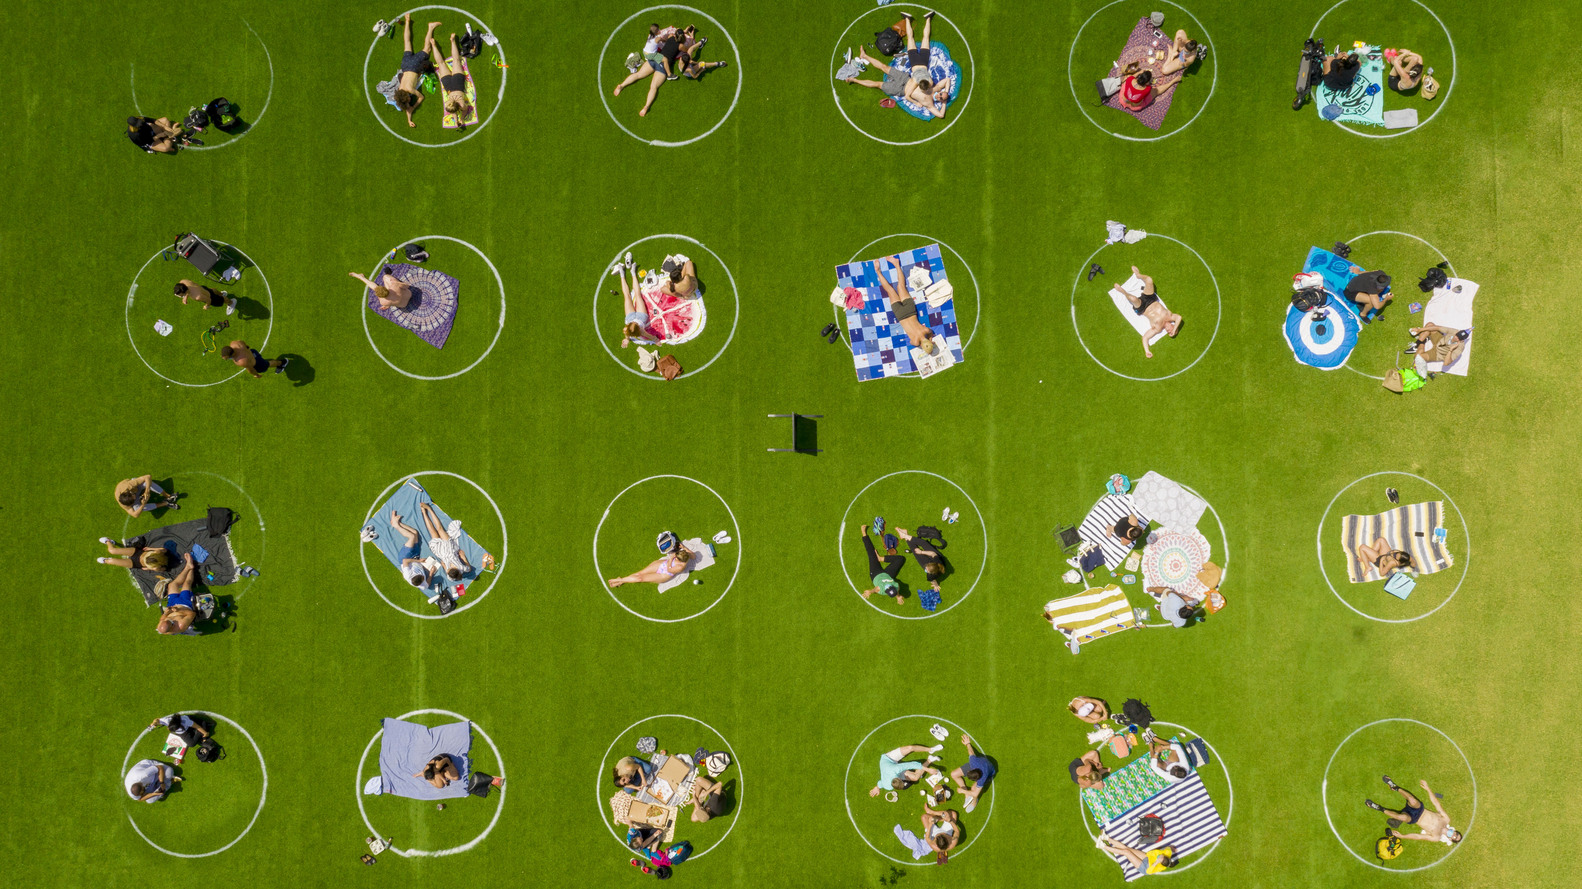
\includegraphics[width=0.9\textwidth]{images/gatherings/domino_park.jpeg}
  \captionsetup{width=0.9\linewidth}
  \caption[Domino Park, NYC]{At Domino Park in New York City, painted circles encouraged social distancing in May 2020 \cite{cogley_white_2020}.}
  \label{fig:domino_park}
\end{figure}

\begin{multicols}{2}

\section{Low-risk social gatherings}
\subsection{Domino Park case study}
In March and April of 2020 when COVID-19 was rapidly spreading in New York City, infection rates and insufficient hospital capacities led to an alarmingly high number of fatalities, instilling a fear that prevented many residents from leaving their homes \cite{thompson_covid-19_2020}. Then, as new infections slowed and people began to emerge from their homes, the park director of Domino Park in New York City decided to reconcile the opposing needs of social distancing and social interaction \cite{strauss_how_2020}. On May 15, 2020, circles were drawn with chalk paint on the grass lawn of Domino Park, eight-feet (2.4 meters) in diameter and six feet apart (1.8 meters) (see Figure \ref{fig:domino_park}) \cite{cogley_white_2020}. 

The dimensions of the Domino Park social gathering circles allow one to four households (one to four individuals per circle) to socialize while maintaining two-meters of physical distance, as depicted in Figure \ref{fig:circle_dims}. Moreover, and importantly during a pandemic, the physically drawn circle provides a sense of enclosure or personal space that reminds park visitors of public health recommendations to maintain low-risk social gatherings. While the size and spacing of the Domino Park circles could be the subject of their own research, this study will make use of the dimensions described above to test the existing capacity of social gatherings in other city parks. 

Furthermore, although socialization typically occurs between at least two people, the analysis that follows will include gathering circles occupied by just one person or a single household. Even without a pandemic, there are individuals who use a park alone and feel comfortable sitting near other visitors even without interacting \cite{peters_social_2010}. Therefore, it can be assumed that during the heightened stress of a pandemic, some people would make use of the gathering circles to enjoy the park in the comfort of their own outdoor space, while surrounding by others doing the same.
\end{multicols}

%\begin{multicols}{2}

%\end{multicols}

\begin{figure}[h]
  \centering
  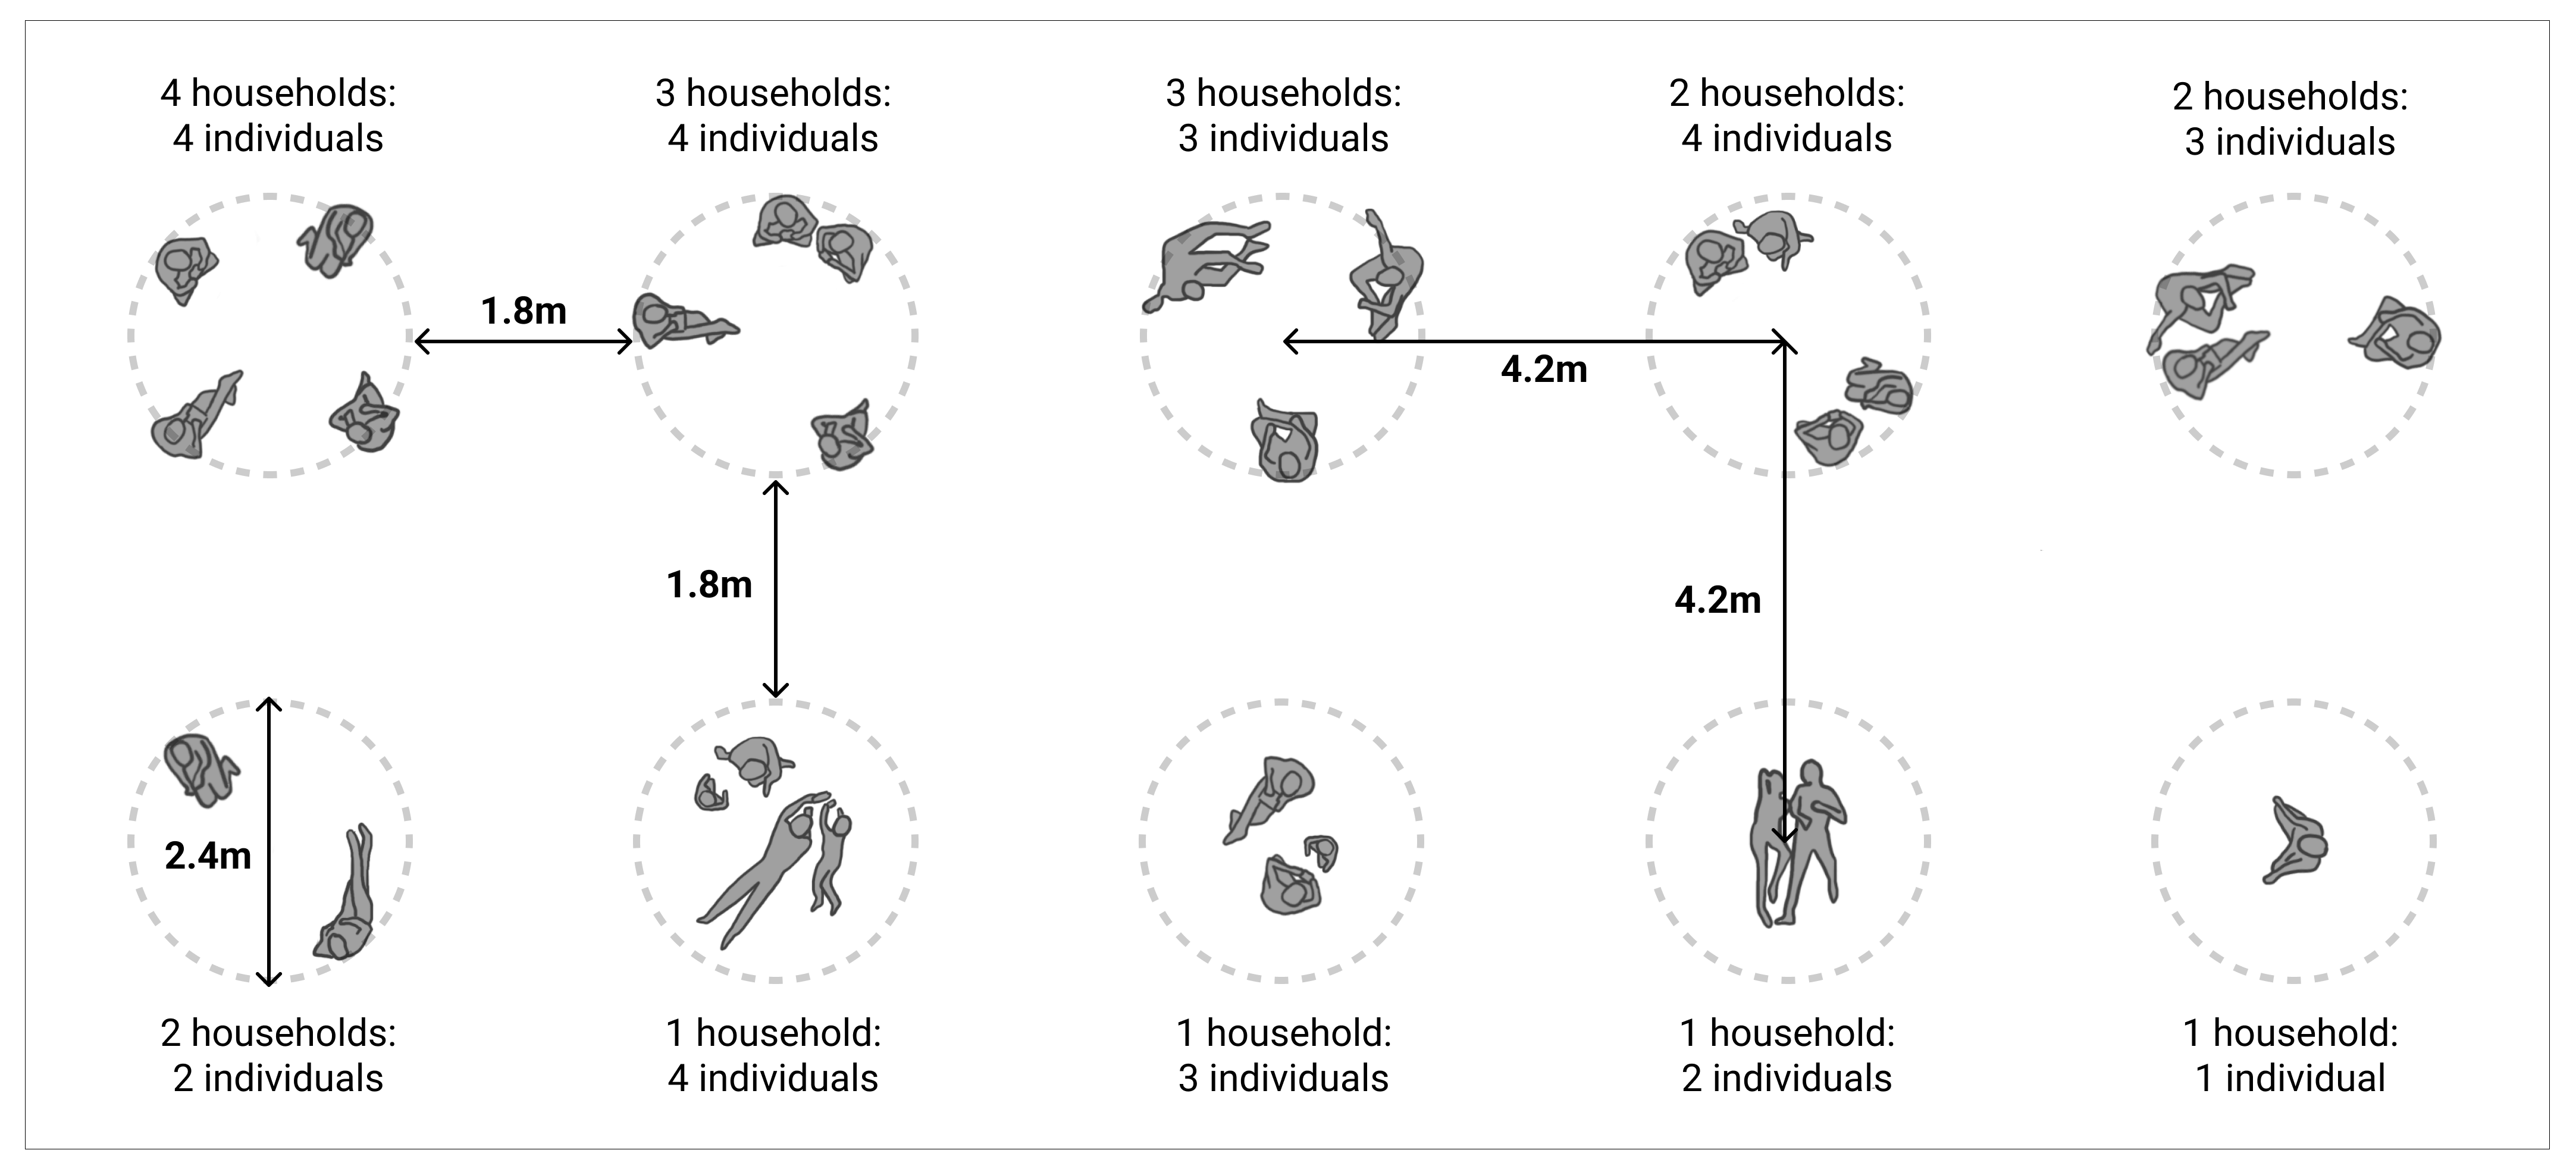
\includegraphics[width=0.9\textwidth]{images/gatherings/circle_dims.png}
  \captionsetup{width=0.9\linewidth}
  \caption[Outdoor gathering circles]{Using the dimensions from Domino Park, this diagram illustrates how social distancing circles can be used by different groups.}
  \label{fig:circle_dims}
\end{figure}

\begin{multicols}{2}

\subsection{Park programming}
The Domino Park social gathering circles are an important case study because they are a proactive yet minimal change to the programming of a park. Many prominent city parks were built early in the last century and funding even for maintenance can be scarce, meaning major design changes do not occur often \cite{havens_parkscapes_2011}. While this research will not propose changes to park programming or design, future studies could use the social gathering quantities discovered below compared to the population studies in Chapter \ref{chapter_05} to advocate for changes that would increase the social gathering capacity of the parks in this study. 

Parks are designed, by necessity, with entry points along the perimeter and with the main internal programming of the park relatively inaccessible except by foot. This allows visitors to feel like they are in nature and far away from the city, but it also means that the distance to the conveniences of the city can be felt \cite{jones_lungs_2018}. Cranz (1989) describes how even for park visitors in the early twentieth century, the expectation was that a day in the park would include amenities such as refreshments, restrooms, lighting, and benches \cite{cranz_politics_1989}. 

The parks in this study are large in area, ranging from 0.56 to 1.8 square kilometers, which means the entrances along the perimeter are not an insignificant walking distance to interior areas suitable for social gatherings. Once visitors enter the park, leaving the park to get food---at a restaurant, food shop, or home---would typically signal the end of the park visit due to the travel distance and time it would take to accomplish those tasks and then return. Therefore, it is assumed that many park visitors who have planned a social gathering in advance would acquire food before entering the park. Typically, large parks contain on-site refreshments, but since maximum capacity of the park is of interest as well as the visitors' variety of options, the next chapter will include sourcing food for social gatherings from outside the park as well as within (see Chapter \ref{chapter_05}).

\section{Research conditions}
\subsection{Where to have an outdoor gathering}
While the most essential criteria for an outdoor social gathering is to be outdoors, there are many factors that contribute to the human comfort and therefore probability of such an event. First, the space must be public and open for people to use at their leisure during the day. This study has not included parks that demand an entrance fee, because even if minimal, a fee reduces the number and equity of potential visitors. Furthermore, while many public plazas could fit most of the conditions below, parks are more often used and more suitable for outdoor gatherings \cite{thorsson_thermal_2007}. Even though picnic tables and benches are part of the landscape of a park, this study will focus on areas where visitors can sit directly on the ground. The additional conditions below will define a suitable outdoor social gathering space for the purpose of this study.

\subsection{Conditions for an outdoor gathering}\label{conditions}
\textit{Grass or non-pavement ground cover}\\
The surface of the ground is an important feature for determining gathering locations. Hard surfaces such as pavement are uncomfortable for long periods of time, and therefore roads and paved paths will not be included for potential gathering areas. Ideally the ground is grass or a similarly soft surface, and not an excessively moisture-absorbing or heat-absorbing material (both sand and turf are less ideal than natural grass for this reason). 

\textit{Larger than 100 square meters in area}\\
Many sources have suggestions for the ideal size of public space. The goal in defining a minimum area for social activities is to eliminate areas of a park that might be identified as suitable for a social gathering by image classification software, but would not in reality be used by park visitors due to the remoteness or scale. The New York Planning Department uses a minimum public plaza size of 2000 square feet, or about 185 square meters \cite{noauthor_privately_nodate}. UNhabitat recommends an area of 0.03 to 0.04 hectares (300 to 400 square meters) for the smallest category of public space called "local/pocket open public spaces" \cite{noauthor_public_nodate}. Zagora and Šamić (2021) use a minimum dimension of 25 meters to define small and extra-small scale public spaces presented in their study \cite{zagora_urban_2021}. Similarly, Gehl (2011) describes 20 to 25 meters to be a socially interesting and relevant distance because it becomes possible to perceive the feelings of surrounding people \cite{gehl_life_2011}. For the purpose of this study any area smaller than 100 square meters is not included in the analysis. 

\textit{No gatherings on sports fields or courts}\\
In the context of a pandemic, playing sports outdoors is generally a low-risk transmission activity similar to an outdoor social gathering. Athletes should therefore still be able to use these program areas for their intended purpose, even if they contain grass lawns which could be used for social gatherings instead. Sports fields will not be analyzed for their social gathering capacity in this study.

\textit{No gatherings within 50 meters of main roads}\\
The parks chosen for this study are large parks that provide visitors with a sense of nature and escape from the city. Because they are all located in dense cities, they are all surrounded by major roads. Gehl (2011) coined the term 'pedestrian city,' for which a distance of 50-100 meters is recommended to transfer from a vehicular landscape (city limits or edge of a residential area) to the local neighborhood \cite{gehl_life_2011}. For this reason, a distance of 50 meters from major roads is utilized to create a visual and auditory barrier between car traffic and the park experience. 

\textit{No gatherings within 10 meters of buildings}\\
Similar to above, most visitors to a park want to feel as if they are in nature, and being near a building would disrupt this feeling. A distance of 10 meters from the exterior of any ancillary park building is recommended based on observations at Yoyogi Park.

\textit{Weather determines sun/shade preferences}\\
While many attributes of Hyde Park, Prospect Park and Yoyogi Park are similar, the most divisive difference is their geographic locations, which create vastly different climatic conditions. Section \ref{thermal_comfort} will determine how thermal comfort informs the ideal locations for outdoor social gatherings in each of these parks.

\vspace{5pt}
\begin{minipage}{0.45\textwidth}
    \centering
    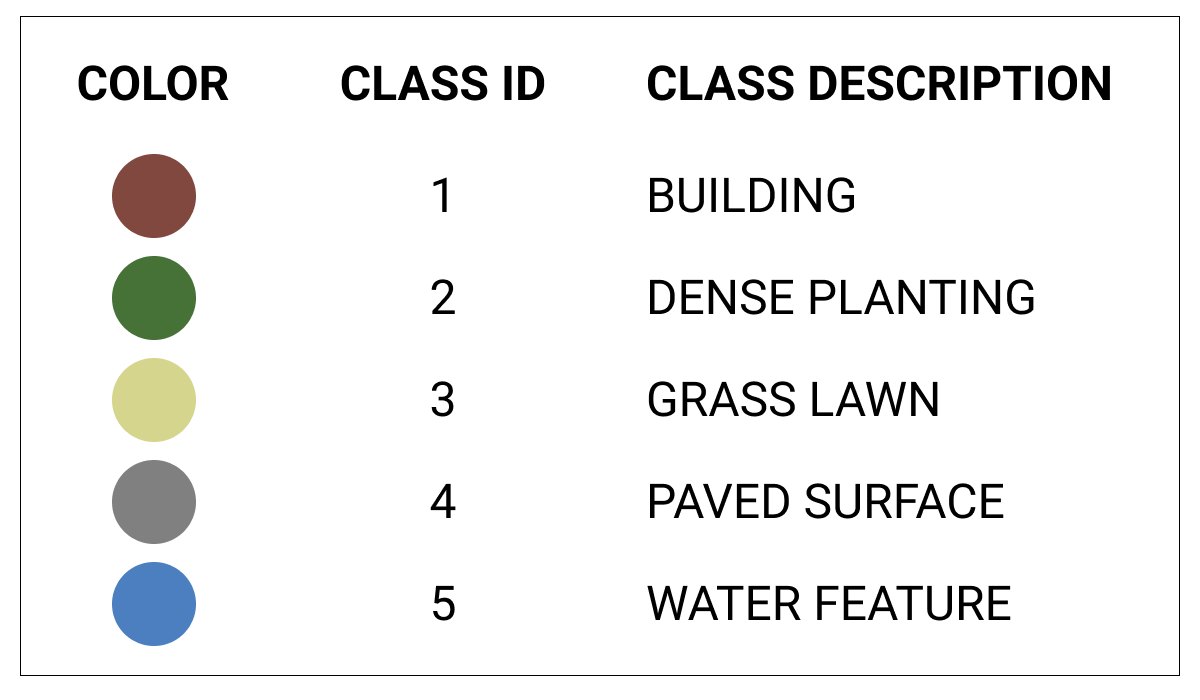
\includegraphics[width=\linewidth]{images/gatherings/OBIA_legend.png}\par\captionof{figure}[Image classification legend]{Image classification legend for the land-cover categories used in this study.}
    \label{fig:obia_legend}
\end{minipage}
\vspace{5pt}

\section{Methodology}
\subsection{Image classification}
Object-based image classification is a technique that uses aerial remote sensing data for land-cover classification \cite{ma_review_2017}. In this study, Google Earth aerial imagery and QGIS tools are used together to locate areas that meet the previously described conditions for social gatherings in the chosen parks \cite{noauthor_google_nodate}. Specifically, the Orfeo ToolBox (OTB) in QGIS is a remote sensing image processing tool that uses segmentation to convert groupings of raster pixels into vector objects that represent different land features \cite{neteler_compiling_2015}. 

While complex techniques for achieving highly accurate image classification results are described by Ma et al. (2017), this research uses sample points for five land-cover categories (see Figure \ref{fig:obia_legend}) to generate predicted values for the segmented vector objects \cite{ma_review_2017}. The land-cover categories include: (1) Building, (2) Dense planting (forest), (3) Grass lawn, (4) Paved surface (road), and (5) Water feature. Once the predicted values are generated, the resulting vector file is manually compared to the original aerial imagery and adjusted where the results are significantly different from the actual attributes of the park. Figure \ref{fig:obia_parks} shows the final adjusted classification results for Hyde Park, Prospect Park, and Yoyogi Park. 

\begin{minipage}{0.45\textwidth}
    \centering
    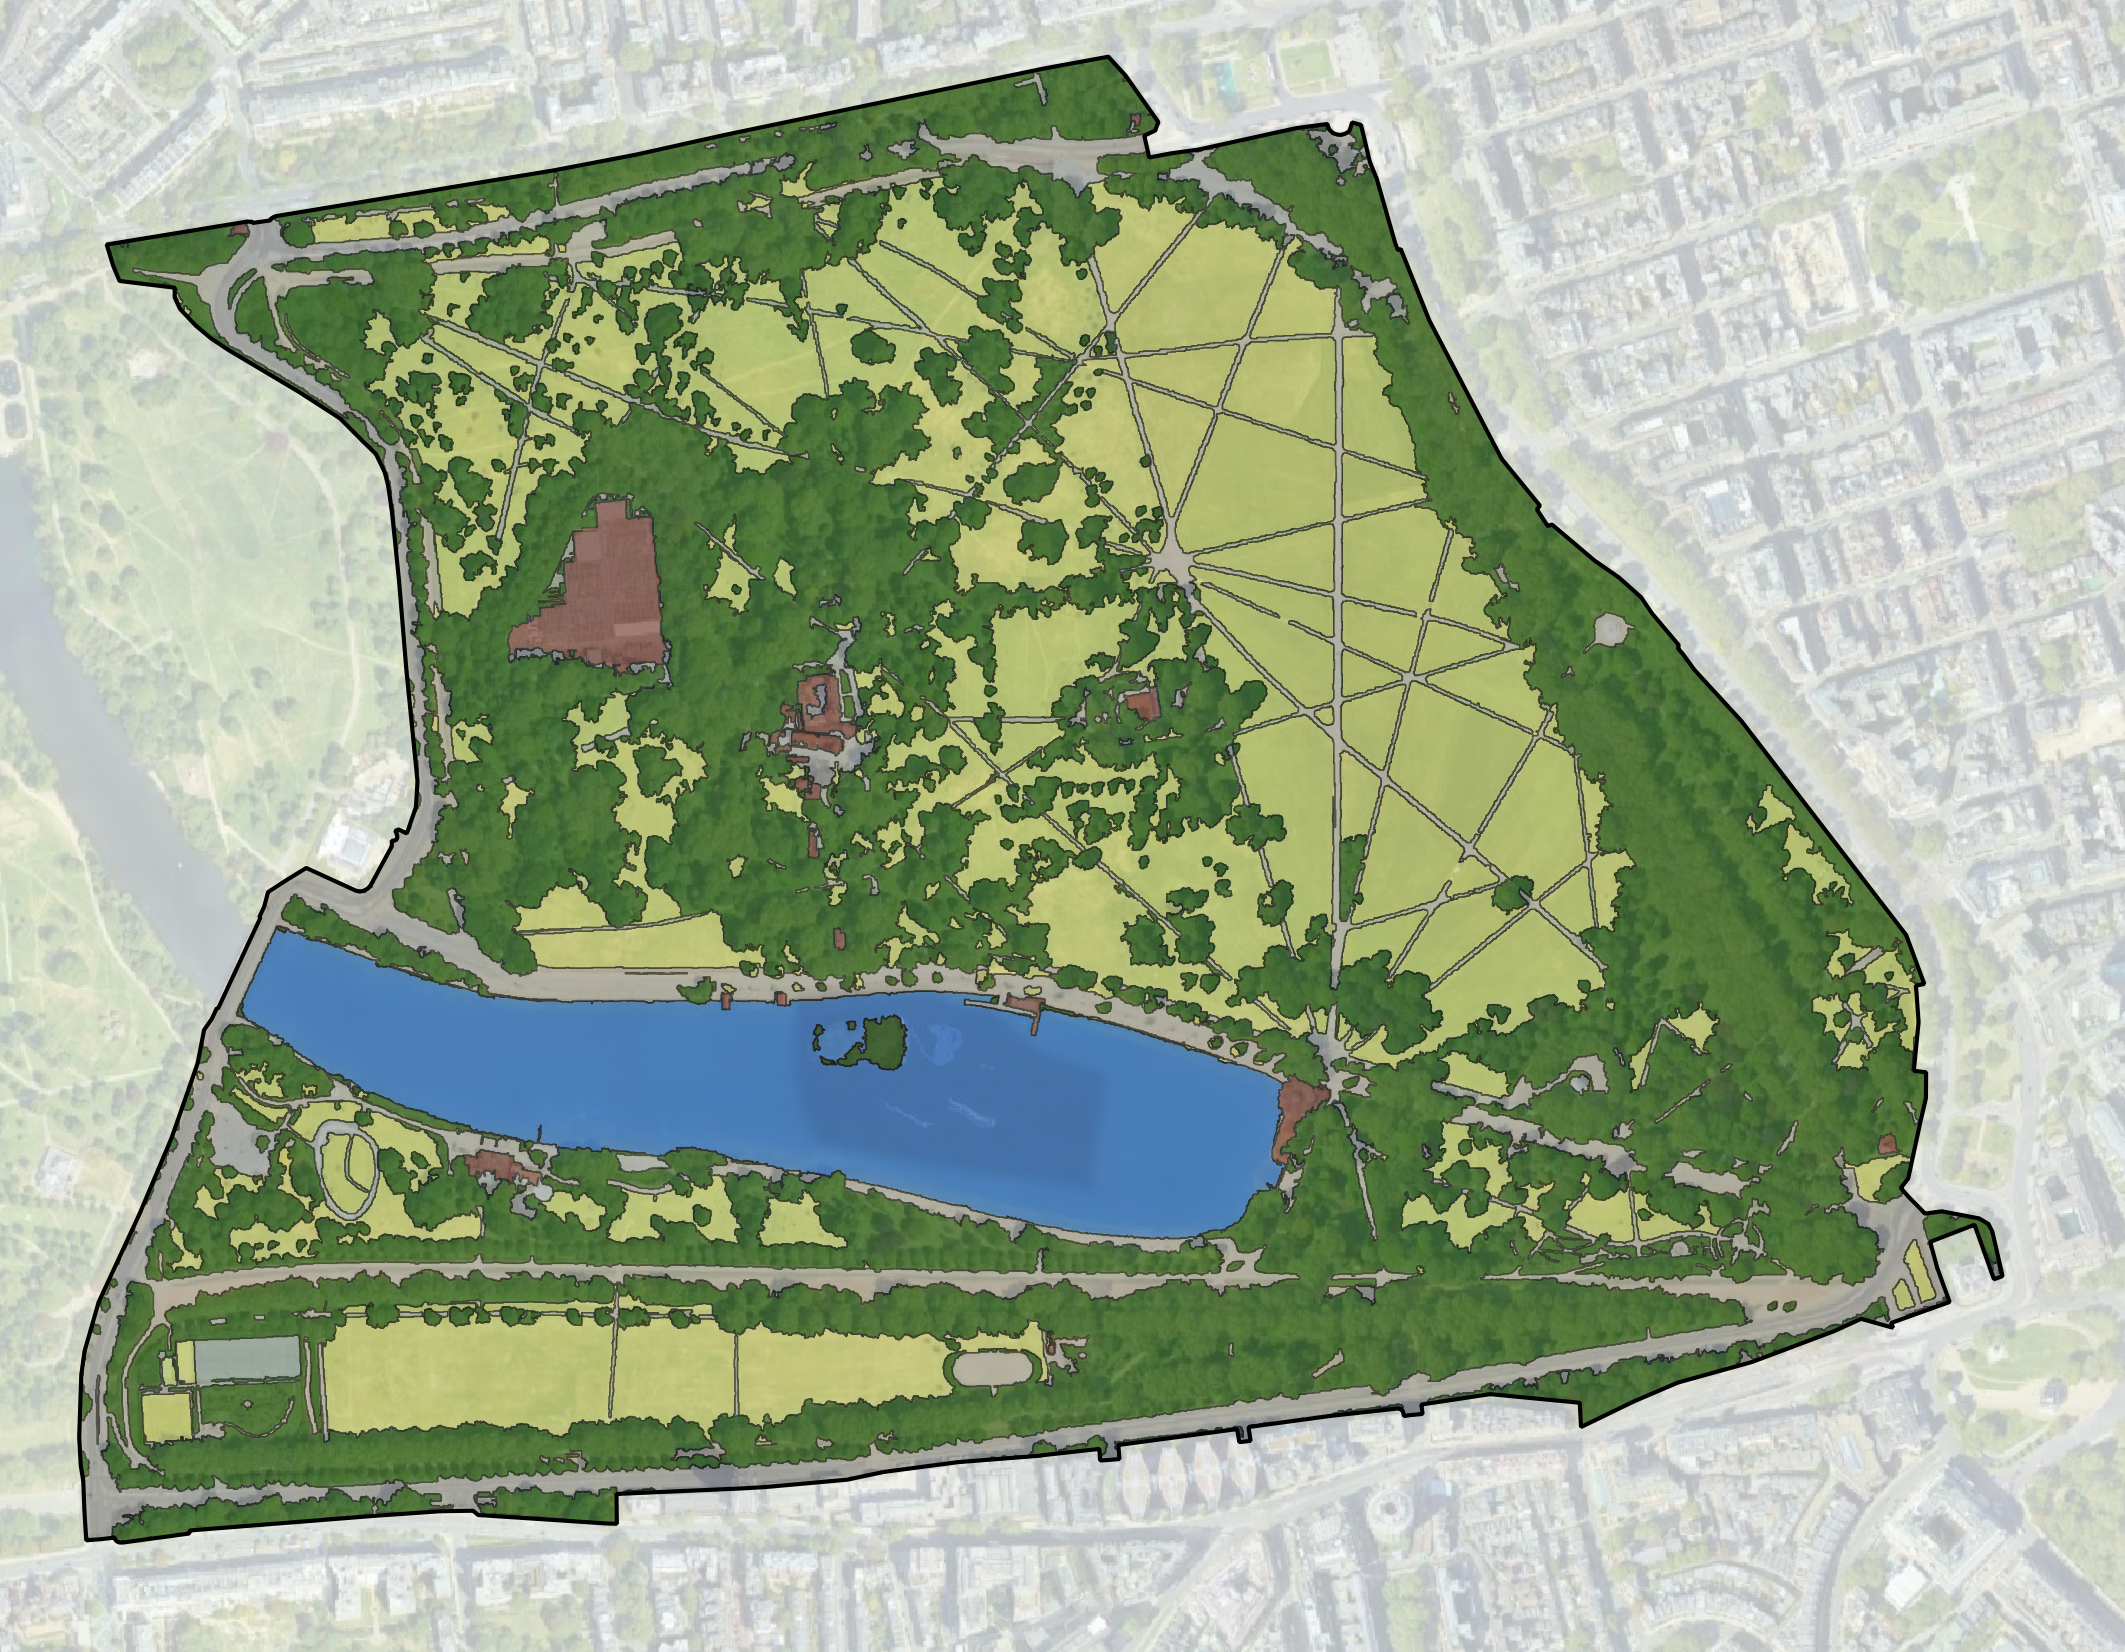
\includegraphics[width=\linewidth]{images/gatherings/hyde_OBIA.png}\par\hspace{5pt} 
    \includegraphics[width=\linewidth]{images/gatherings/prospect_OBIA.png}\par\hspace{5pt} 
    \includegraphics[width=\linewidth]{images/gatherings/yoyogi_OBIA.png}\par\hspace{5pt} 
    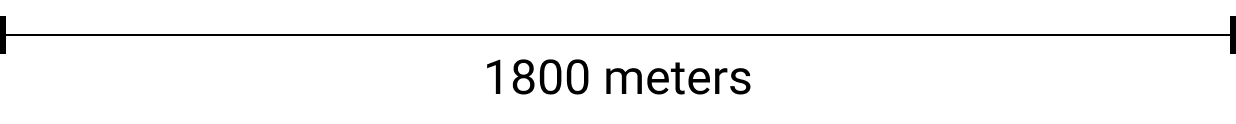
\includegraphics[width=\linewidth]{images/gatherings/scale_legend.png}\par\captionof{figure}[Image classification]{Top to bottom: Hyde Park, Prospect Park, and Yoyogi Park. Object-based image classification by land-cover category.}
    \label{fig:obia_parks}
\end{minipage}

\end{multicols}

\begin{figure}[h]
  \centering
  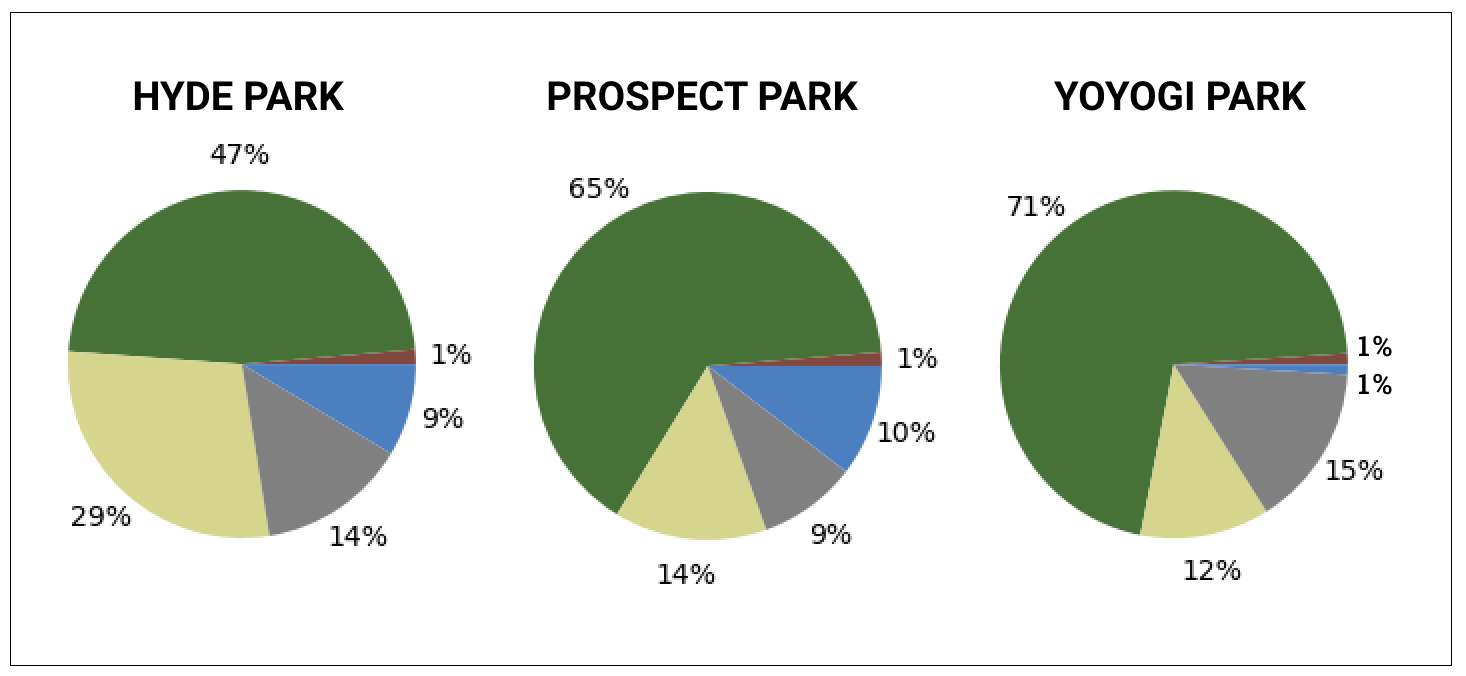
\includegraphics[width=0.7\textwidth]{images/gatherings/pie_charts.png}
  \captionsetup{width=0.7\linewidth}
  \caption[Classification pie charts]{Pie charts representing the percentage of park area for each land-cover category from the adjusted image classification models.}
  \label{fig:pie_charts}
\end{figure}\par
\vspace{5pt}

\begin{table}[h]
    \centering
    \small
    \begin{tabular}{lcrrrr}
    \toprule
    Park Name &  Class &  Predicted &  Adjusted & Percent & Percent\\
     &  ID &  Area $ (m^{2}) $ &  Area $ (m^{2}) $ & Change & of Park\\
    \midrule
    Hyde Park &         1 &           44275 &          18749 &     -57.65\% &                       1.35\% \\
     &         2 &          683667 &         659413 &      -3.55\% &                      47.48\% \\
     &         3 &          378250 &         398761 &       5.42\% &                      28.71\% \\
     &         4 &          152996 &         192620 &       25.9\% &                      13.87\% \\
     &         5 &          129711 &         119356 &      -7.98\% &                       8.59\% \\
    \midrule
    Prospect Park &         1 &           82665 &          23021 &     -72.15\% &                       1.28\% \\
     &         2 &         1157466 &        1172324 &       1.28\% &                      64.98\% \\
     &         3 &          264518 &         256300 &      -3.11\% &                      14.21\% \\
     &         4 &          105981 &         165239 &      55.91\% &                       9.16\% \\
     &         5 &          193539 &         187285 &      -3.23\% &                      10.38\% \\
    \midrule
    Yoyogi Park &         1 &           34684 &           5659 &     -83.68\% &                       1.01\% \\
     &         2 &          379617 &         397461 &        4.7\% &                       70.9\% \\
     &         3 &           99354 &          67473 &     -32.09\% &                      12.04\% \\
     &         4 &           42377 &          84667 &      99.79\% &                       15.1\% \\
     &         5 &            4536 &           5308 &      17.02\% &                       0.95\% \\
    \bottomrule
    \end{tabular}
    \caption[Predicted and adjusted image classification]{Predicted versus adjusted areas of the image classification analysis.}
    \label{table:OBIA}
\end{table}

\begin{multicols}{2}

\subsection{Classification results}
Although the attributes such as area and geographic location vary, each park contains grass lawns, forested areas, water features, sports facilities, ancillary buildings, roads and pedestrian paths. Figure \ref{fig:pie_charts} shows the percentage of coverage for the above-mentioned land-cover categories in each park, giving an initial point of comparison for how much space might be available for social gatherings. Each of the parks contain only one-percent of land dedicated to buildings, showing that the three parks likely have similar proportions of ancillary facilities dedicated to restrooms, concessions, and maintenance equipment. Hyde Park contains the highest proportion of grass lawn (29\%) and largest area (almost 400,000 square meters), followed by Prospect Park with roughly 256,000 square meters of grass lawn or 14\% of the whole park. Yoyogi Park has less than 70,000 square meters of grass lawn or 12\% of the park area; however, Yoyogi Park has the highest proportion of forest (dense planting) with 71\%, which increases the number of potential social gathering spaces due to the climate in Tokyo and the culture preferences for less sun (see Section \ref{thermal_comfort}). 

Shaori et al. (2020) uses the two-meter social distancing requirements to create a metric of four square meters per person in calculating the distribution of green space across England and Wales. While this would mean that a park the size of Hyde Park (1.4 square kilometers) would potentially reach a capacity of 350,000 visitors, this is unrealistic because 52\% of the park is dedicated to water features, roads, buildings, and dense planting areas as determined by the image analysis above. By identifying plausible social gathering areas, this study aims to find a more accurate predictor of the capacity of city parks. 

\subsection{Accuracy verification}
The accuracy of the image classification can be seen in Figure \ref{fig:obia_diff} using the legend in Figure \ref{fig:accuracy_legend}. To understand which categories were the most and least likely to be correctly identified, the percent change is calculated in Table \ref{table:OBIA} of the computer-predicted to the manually-adjusted areas. For Hyde and Prospect parks, the two categories that present the least change between predicted and adjusted models are Class (2) Dense planting and Class (3) Grass lawn. For all three parks, the two most incorrectly identified categories are (1) Buildings and (4) Paved surfaces. Because Class (2) and (3) are more important to this study, it is significant to note that these two classifications are generally predicted accurately.  

Finally, an overall accuracy value is determined in Table \ref{table:global_OBIA} by taking the percentage of the area of correctly identified vector objects compared to the total area of each park. Prospect Park is the most accurate model at 95\% and Yoyogi Park is the least accurate at around 83\%. This is likely due to the aerial imagery used, as the most recent Google Earth imagery for Yoyogi Park is from a winter month. In the image, the trees do not have leaves and therefore the image classification tool can not easily differentiate the trees from the ground surface. On the other hand, Prospect Park's imagery is from a summer month, so the contrast between the dark green of the trees and light green of the grass lawns is easily distinguished by both the computer and the human eye.

\begin{minipage}{0.45\textwidth}
    \centering
    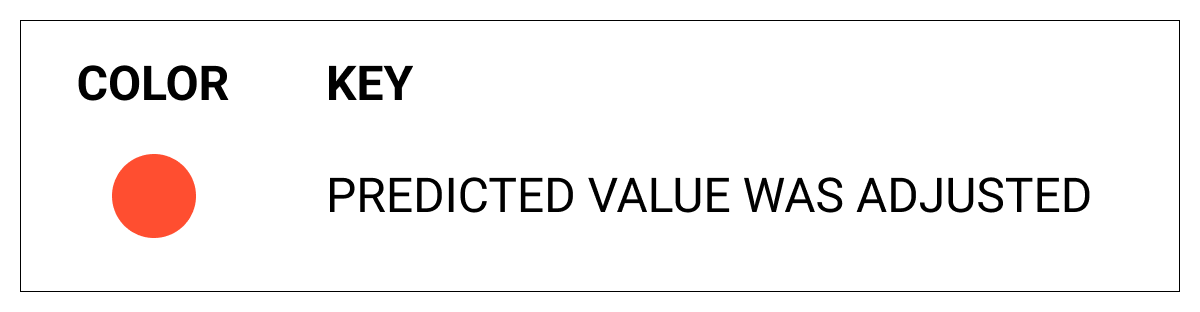
\includegraphics[width=\linewidth]{images/gatherings/accuracy_legend.png}\par\captionof{figure}[Image classification accuracy legend]{Legend for the accuracy models of image classification analysis.}
    \label{fig:accuracy_legend}
\end{minipage}

\begin{minipage}{0.45\textwidth}
    \centering
    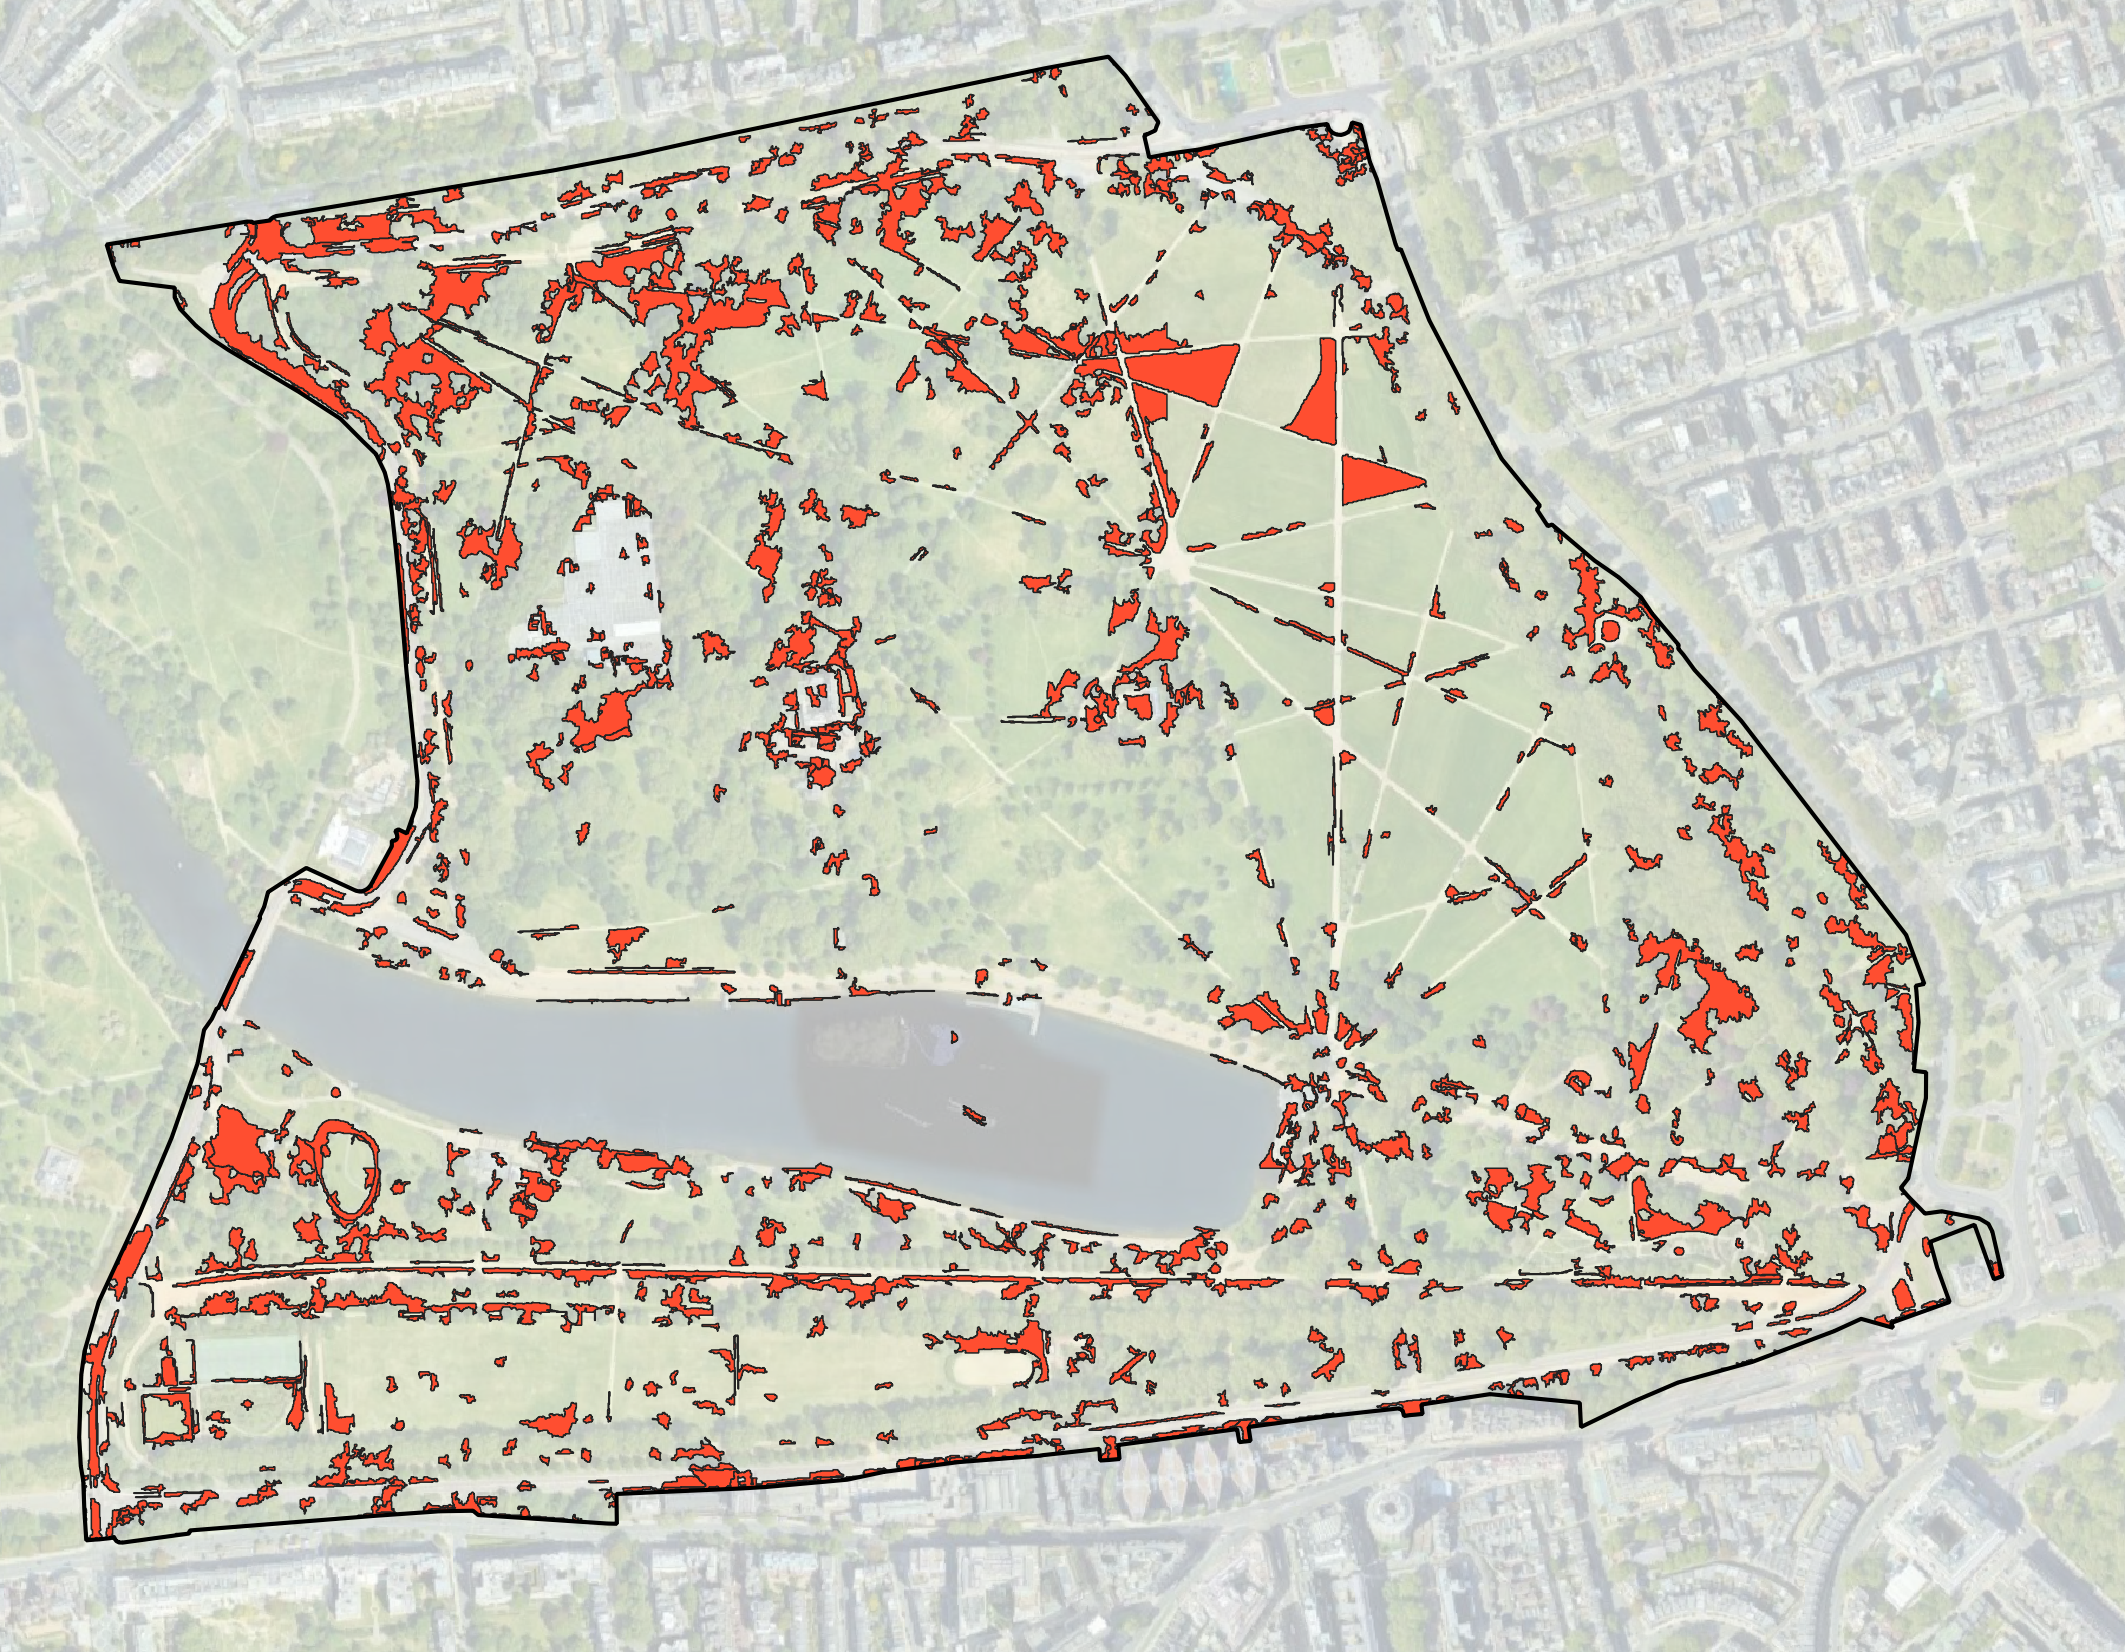
\includegraphics[width=\linewidth]{images/gatherings/hyde_OBIA_diff.png}\par\hspace{5pt} 
    \includegraphics[width=\linewidth]{images/gatherings/prospect_OBIA_diff.png}\par\hspace{5pt} 
    \includegraphics[width=\linewidth]{images/gatherings/yoyogi_OBIA_diff.png}\par\hspace{5pt} 
    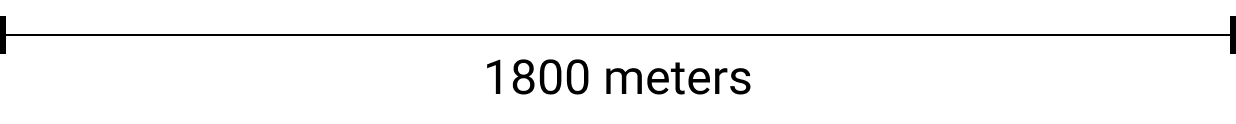
\includegraphics[width=\linewidth]{images/gatherings/scale_legend.png}\par\captionof{figure}[Image classification accuracy]{Top to bottom: Hyde Park, Prospect Park, and Yoyogi Park. Discrepancies between predicted and adjusted image classification.}
    \label{fig:obia_diff}
\end{minipage}

\end{multicols}

\begin{table}[h]
      \centering
      \small
    \begin{tabular}{lr}
    \toprule
    Park Name &  Overall Accuracy \\
\midrule
Prospect Park &     95.07\% \\
Hyde Park &     87.97\% \\
Yoyogi Park &     83.36\% \\
    \bottomrule
    \end{tabular}
    \caption[Image classification accuracy table]{Overall accuracy of object-based image analysis for each park.}
    \label{table:global_OBIA}
\end{table}

\begin{multicols}{2}
\section{Outdoor thermal comfort}\label{thermal_comfort}
The next prerequisite to locating the ideal outdoor social gathering is understanding thermal comfort, which is a vast and complex topic that changes based on the climate. Several studies have shown that parks have cooler temperatures than their surrounding urban environments, meaning choosing a park for an outdoor activity is advantageous in warmer weather compared to other outdoor spaces \cite{spronken-smith_thermal_1998}\cite{cohen_methodological_2014}. Additionally, thermal comfort in parks has been studied by many scholars, including Gehl (1996), Thorsson et al. (2007), Nikolopolou et al. (2001), and Matzarakis and Mayer (1997), and preferences for sun versus shade has been correlated to certain temperature ranges which will be used in the analysis that follows \cite{gehl_life_2011}\cite{thorsson_thermal_2007}\cite{nikolopoulou_thermal_2001}\cite{matzarakis_applications_1999}. Throughout the year, each city in this study (London, New York City, and Tokyo) will experience days when using a park for a social gathering is unpleasant if not impossible, due to precipitation, extreme cold or heat, and even air quality. However, on the days where the conditions are within the acceptable thermal comfort ranges, dressing appropriately and taking advantage of either solar exposure or shading can expand the potential for gatherings in a park. 

Physiological equivalent temperature (PET) was introduced by Höppe and Mayer in 1987 as the temperature at which the human body balances heat in an indoor setting with some physical movement and clothing. The calculated PET values consider air temperature, mean radiant temperature, wind velocity, and vapor pressure \cite{hoppe_physiological_1999}. Sunny and shaded areas under the same air temperature result in different PET values due to solar exposure (or lack thereof). For example, a sunny, summer day of 30$^{\circ}$ Celsius and a vapor pressure of 21 hPa creates a 43$^{\circ}$ Celsius physiological equivalent temperature for the human body. However, if that same person moved into the shade, the resulting PET would be 29$^{\circ}$ Celsius, a significant difference \cite{hoppe_physiological_1999}. 

\end{multicols}

\begin{figure}[H]
  \centering
  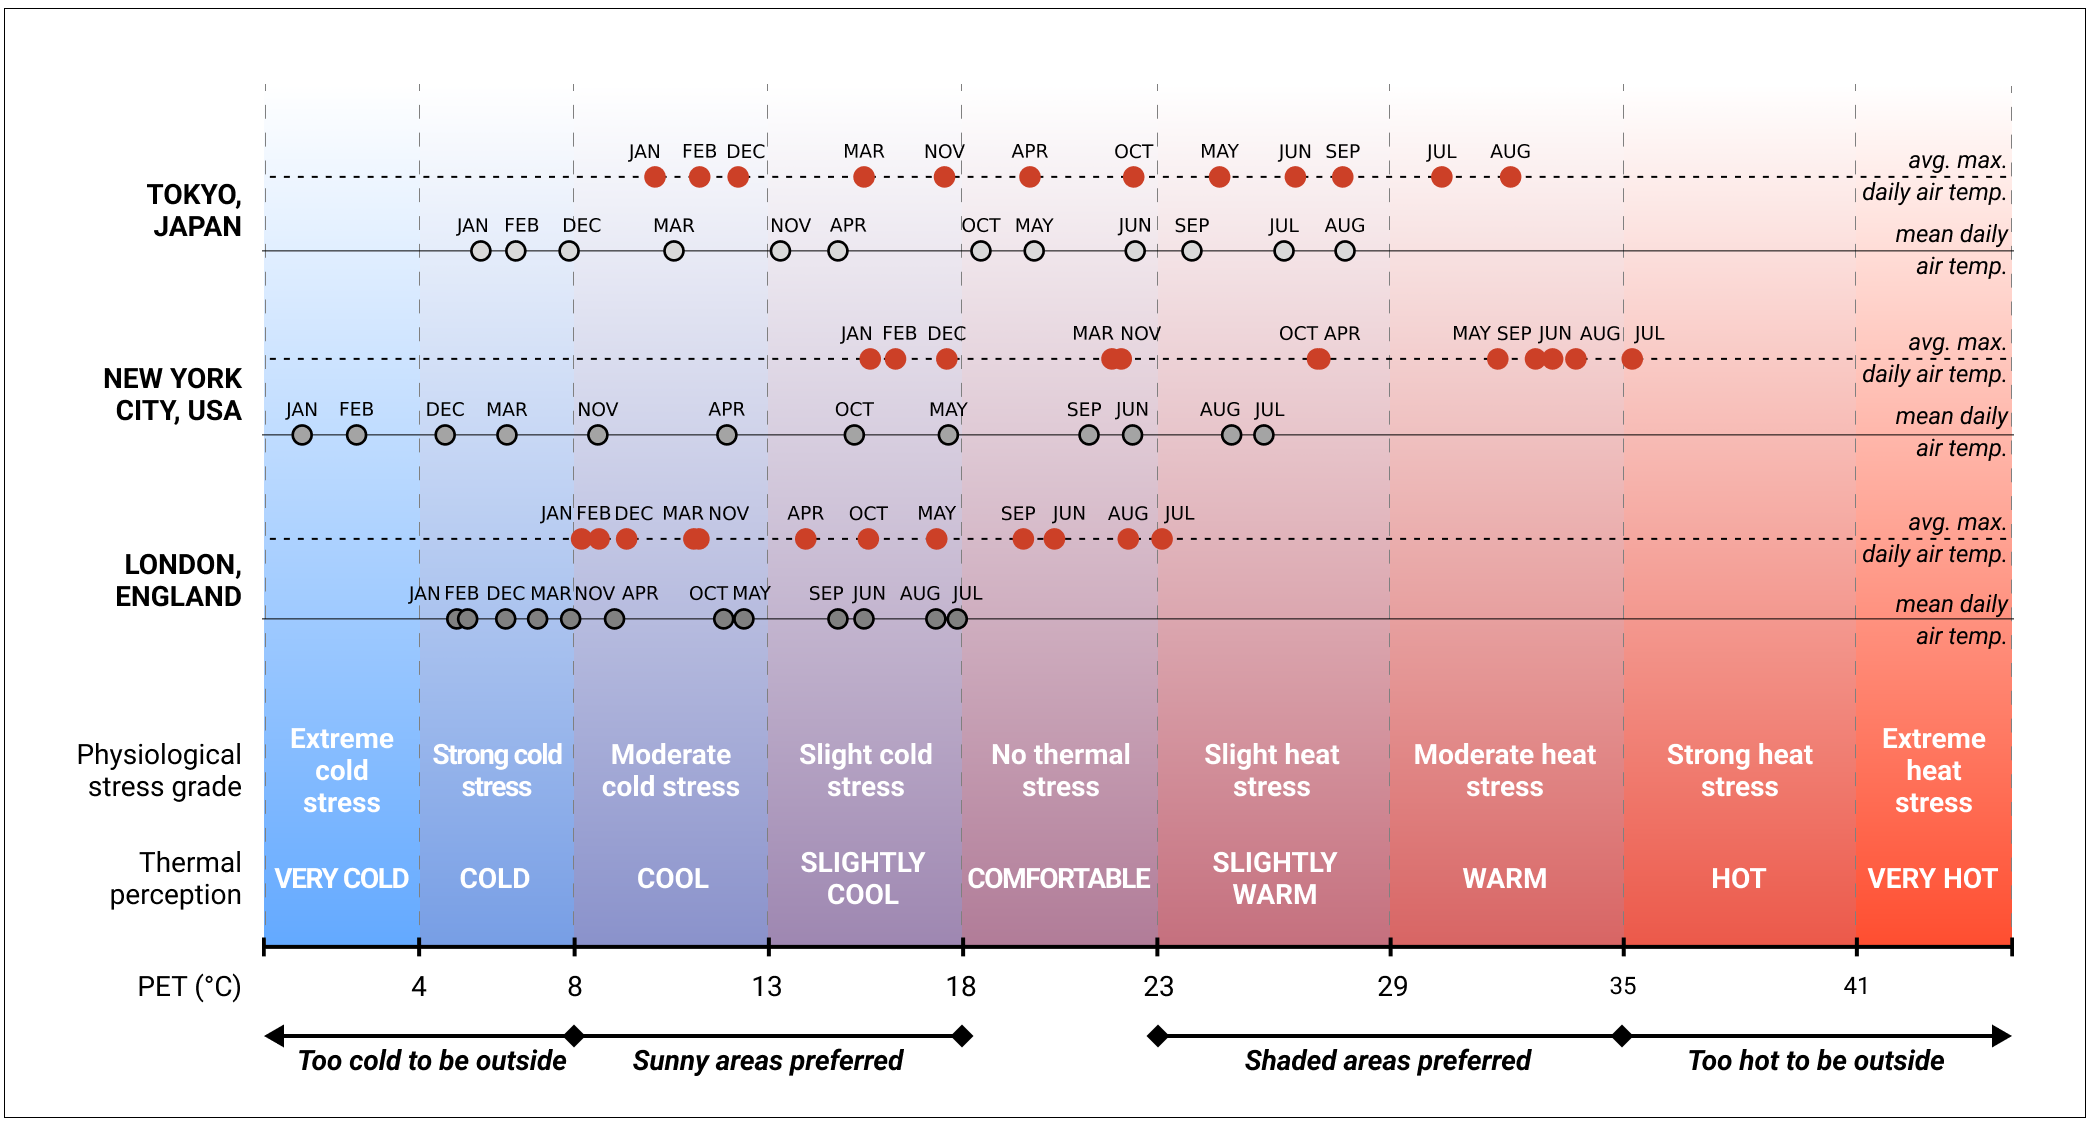
\includegraphics[width=1.0\textwidth]{images/gatherings/temperature.png}
  \caption[Average temperatures by month]{Monthly mean and maximum daily air temperatures in degrees Celsius (data averaged from 2012-2022) compared to physiological stress and thermal perception as defined by Matzarakis et. al (1999) \cite{matzarakis_applications_1999}. See Appendix C for more information.}
  \label{fig:temperature}
\end{figure}

\begin{table}[H]
\begin{adjustwidth}{-1in}{-1in} % Adjust margins to center the table
\small
\centering
\begin{tabular}{lccccccccr}
\toprule
{}  &  {} &  London &  {}  & {}  &  New York City  &  {}  & {}  &  Tokyo  & {}\\
\midrule
\multicolumn{1}{c|}{} &  Mean &  Max. &  \multicolumn{1}{c|}{} &  Mean &  Max. &  \multicolumn{1}{c|}{} &   Mean  &   Max. &  {} \\
\multicolumn{1}{c|}{Month} &  temp. &  temp. &  \multicolumn{1}{c|}{Humid.} &  temp. &  temp. &  \multicolumn{1}{c|}{Humid.$^1$} &   temp. &  temp. &  Humid. \\
\midrule
JAN &    5.02 &        8.18 &        84\% &    0.99 &      15.61 &      73\% &   5.64 &     10.07 &      52\% \\
FEB &    5.30 &        8.63 &        79\% &    2.39 &      16.26 &      72\% &   6.54 &     11.22 &      53\% \\
MAR &    7.10 &       11.07 &        75\% &    6.26 &      21.83 &      70\% &  10.61 &     15.45 &      60\% \\
APR &    9.08 &       13.95 &        69\% &   11.92 &      27.18 &      67\% &  14.83 &     19.72 &      64\% \\
MAY &   12.41 &       17.32 &        69\% &   17.62 &      31.76 &      67\% &  19.88 &     24.60 &      68\% \\
JUN &   15.50 &       20.35 &        69\% &   22.36 &      33.17 &      69\% &  22.48 &     26.55 &      77\% \\
JUL &   17.90 &       23.12 &        67\% &   25.74 &      35.22 &      69\% &  26.31 &     30.32 &      80\% \\
AUG &   17.35 &       22.25 &        71\% &   24.91 &      33.77 &      73\% &  27.88 &     32.09 &      77\% \\
SEP &   14.83 &       19.55 &        77\% &   21.24 &      32.73 &      75\% &  23.94 &     27.77 &      79\% \\
OCT &   11.89 &       15.56 &        83\% &   15.20 &      27.12 &      73\% &  18.51 &     22.39 &      73\% \\
NOV &    7.95 &       11.20 &        86\% &    8.60 &      22.07 &      75\% &  13.35 &     17.52 &      66\% \\
DEC &    6.28 &        9.34 &        86\% &    4.67 &      17.58 &      76\% &   7.91 &     12.21 &      58\% \\
\bottomrule
\end{tabular}
\end{adjustwidth}
\caption[Average temperature and humidity]{Average daily mean temperature and maximum temperature in degress Celsius and humidity in percentage for London, New York City and Tokyo from 2012-2022.}
\label{table:temp_humidity}
\end{table}

\begin{multicols}{2}

Matzarakis and Mayer (1997) created a PET conversion chart to associate the human sensation (cold, comfortable, hot) and thermal stress level (cold stress, heat stress) to physiological equivalent temperature ranges \cite{matzarakis_urban_1997}. Although PET values can only be calculated if precise micro-climate conditions are known, by comparing air temperatures with these values and knowing the approximate humidity, deductions can be made about the thermal conditions of an outdoor space. 

\subsection{Thermal comfort for social gatherings}
In Cambridge, England, about 80 kilometers Euclidean distance north of Hyde Park, Nikolopoulou et al. (2001) found thermal neutrality in urban spaces to vary from 7.5$^{\circ}$ C in the winter to 27$^{\circ}$ C in the summer. The authors explain that a large component to adjusting to the seasonal weather is clothing layers, as people will dress for colder or warmer conditions in order to be comfortable in the outdoor environment for longer periods of time. They also found a differentiation between users actively moving (exercising, passing through) versus users resting (eating, socializing), where those who were resting preferred sunlight and warm conditions \cite{nikolopoulou_thermal_2001}.

Figure \ref{fig:temperature} shows a comparison of the mean daily air temperature and mean maximum air temperature by month averaged over ten years (2012-2022) for the three cities, compared to the physiological stress grades and thermal perception ratings defined by Matzarakis and Mayer (1997) \cite{matzarakis_urban_1997}. This figure shows that the mean monthly air temperature values for southeast and central south England do not exceed 18$^{\circ}$ Celsius, and the average maximum air temperature by month peaks in July around 23$^{\circ}$ Celsius. Comparing these temperatures to the PET ratings, it can be assumed that for Hyde Park, visitors will tend to sit in sunny areas because shaded areas would be in the range for cold stress most of the year. 

Tokyo has the highest mean temperature in the summer months along with the highest humidity\footnote{Humidity data from New York City is an average from the last twenty years.} values (see Table \ref{table:temp_humidity}), making it unpleasant and at times dangerous to spend time in the sun. A summer day with an air temperature of 32$^{\circ}$ Celsius and humidity of 77\% translate to a heat index of 43$^{\circ}$ Celsius, conditions conducive to heat stroke. In their study located in Matsudo, Japan, located about 22 kilometers Euclidean distance from Yoyogi Park, Thorsson et al. (2007) found that when the temperature was higher than 20$^{\circ}$ Celsius, 80 percent of the visitors sought shade in a park \cite{thorsson_thermal_2007}. Because the months of June through September have average daily air temperatures that exceed 20$^{\circ}$ Celsius, it can be assumed that providing ample shaded areas for social gatherings in Yoyogi Park is a necessity. 

New York City experiences on average higher maximum air temperatures from May to September compared to that of Tokyo (see Figure \ref{fig:temperature}), but the average daily air temperatures remain lower. However, the use of parks and outdoor space is not as inhibited on these high temperature days compared to Tokyo. The differences are influenced by both climate and culture. Thorsson et al. (2007) discuss how culturally western societies (especially in places that experience dark and/or gray winters like New York City and London) tend to favor spending time in the summer sun \cite{thorsson_thermal_2007}. For this reason, shade will be more important to social gatherings in Tokyo compared to London and New York. 

\end{multicols}

\begin{table}[h]
  \centering
\small
\begin{tabular}{lllllll}
\toprule
PET (°C) & Thermal Perception  &    Conditions &  London & New York City & Tokyo &  \\
\midrule
<8 &      Cold/Very cold  &    Not recommended &       42.0\% &    33.0\% &      25.0\%  \\
8 - 18 &  Slightly cool/Cool  &      Sun preferred &       58.0\% &    33.0\% &      25.0\% \\
18 - 23 &         Comfortable  &  Indiv. preference  &        0.0\% &    17.0\% &      25.0\%\\
23 - 35 &  Slightly warm/Warm  &    Shade preferred &        0.0\% &    17.0\% &      25.0\%\\
>42  &        Hot/Very hot  &    Not recommended  &        0.0\% &     0.0\% &       0.0\%\\
\bottomrule
\end{tabular}
\caption[Thermal perception by city]{Percentage of average monthly air temperatures distributed by thermal perception and preferred outdoor gathering conditions.}
\label{table:yearly_percent}
\end{table}

\begin{figure}[h]
  \centering
  \captionsetup{width=1.0\linewidth}
  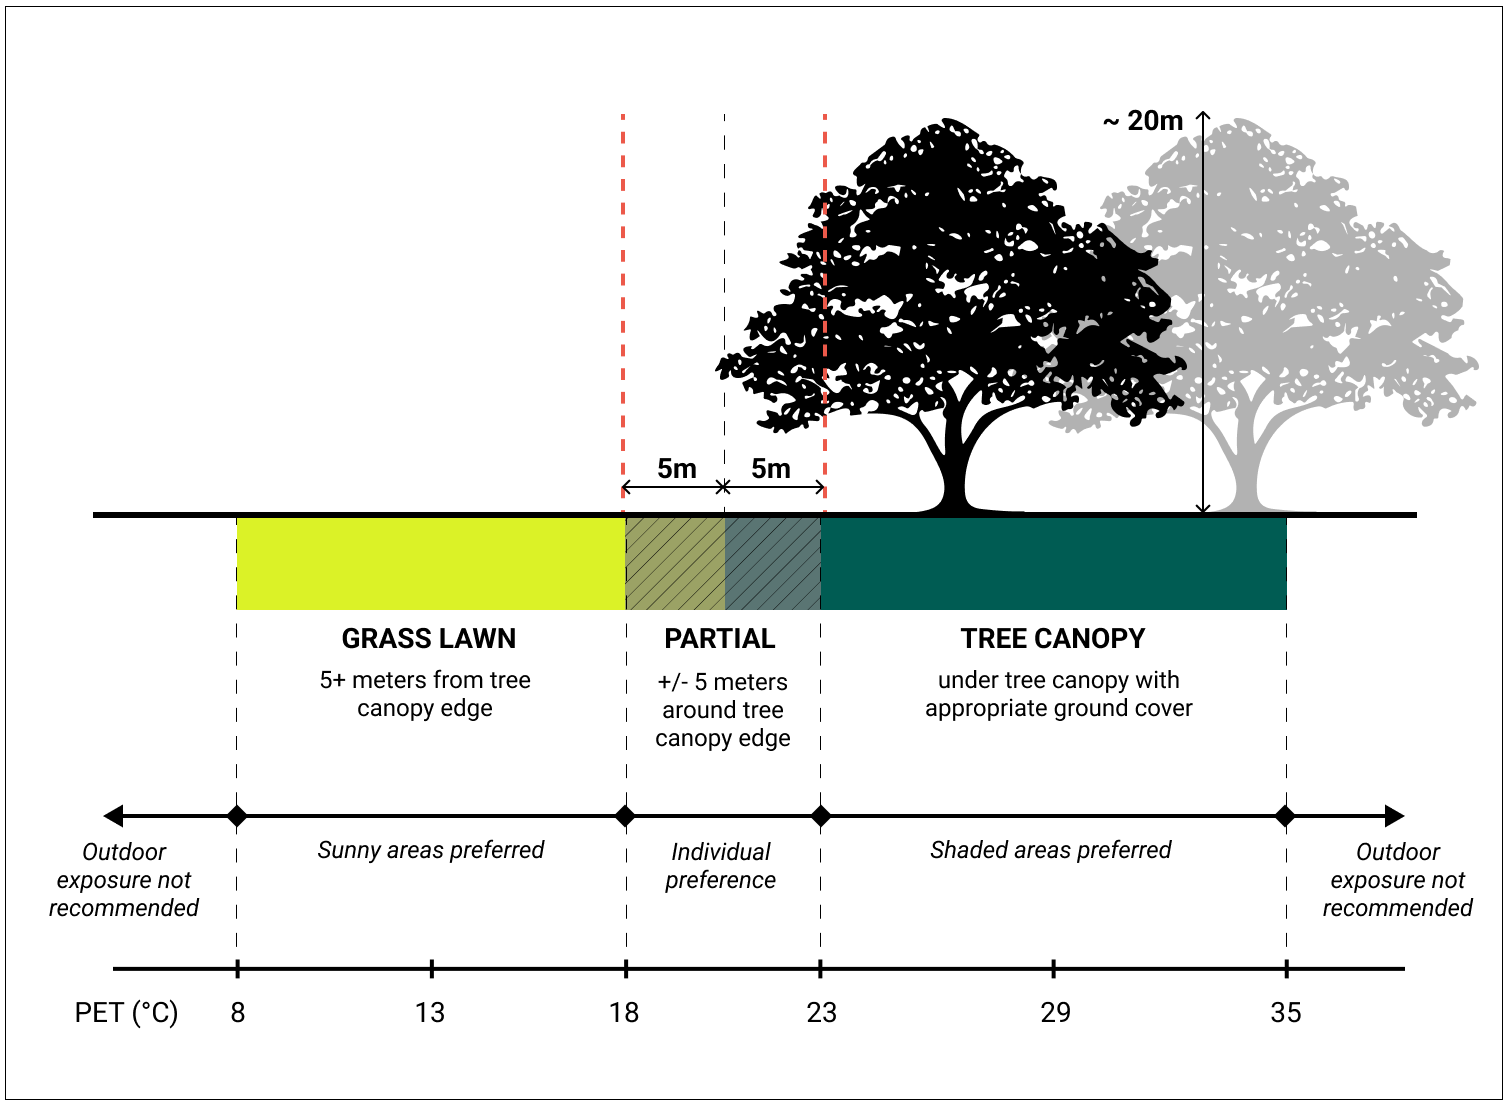
\includegraphics[width=1.0\textwidth]{images/gatherings/shade_sun_trees.png}
  \caption[Shade and Sun Tree Section]{Using thermal perception and physiological stress grade to classify preferable locations for outdoor gatherings and comparing to a cross-section of park conditions.} 
  \label{fig:shade_and_sun}
\end{figure}

\begin{multicols}{2}

\subsection{Gatherings in the shade and sun}
Table \ref{table:yearly_percent} shows the average monthly air temperatures grouped by the thermal perception categories as defined by Matzarakis et. al (1999). From this table, the percentage of the year that park visitors will likely prefer sun or shade can be deduced. For example, Hyde Park in London will have air temperatures below 8$^{\circ}$ Celsius for approximately 42\% of the year. Although these values would change if micro climate data was available to calculate true PET values, this table illustrates how shaded gathering areas will not be sought out most days in London. Tokyo, on the other hand, shows 25\% of the year in the range for "individual preference" of sunny or shaded gathering areas, and 25\% of the year in the range for "shade preferred." Given the previous climatic and cultural discussion, shaded areas for social gatherings in Yoyogi Park will be more important than sunny areas. 

The three zones identified for social gatherings in this study are grass lawn, partial sun/shade and tree canopy. For all three parks, there are days of the year when the outdoor air temperature allows sitting in the sun or shade to be a matter of personal preference. Additionally, each park has an assortment of tree species and vegetation that creates unique ground cover and tree canopy conditions. Under-tree canopy social gatherings will only be analyzed for Yoyogi Park, but the partial sun/shade zone is important to include for all parks. 

The depth of the partial sun/shade zone is an important yet difficult value to determine due to the variety of trees in each park and among the parks. Yoyogi Park's most common trees are the Japanese zelkova (20-24 meters in height), Sawara cypress (35-50 meters) and the Camphor (15-18 meters) \cite{noauthor__nodate}. London Plane trees represent 37\% of the foliage in Hyde Park, ranging in height from 22 to 30 meters \cite{noauthor_i-tree_nodate}. Prospect Park has the largest quantity and variety of vegetation, with over 30,000 trees \cite{tours_trees_2020}. Some of the most common species include the Flowering Dogwood (5-12 meters in height), Sugar Maple (18-24 meters) and the Eastern White Oak (15-30 meters) \cite{says_tree_nodate}. A 15-meter tall tree in Tokyo will cast a shadow of 3 meters at noon on the summer solstice and 25 meters on the winter solstice. An average of 5 meters from the tree canopy edge is used to define the area of partial sun/shade across the three parks, although in actuality direction and depth will vary throughout the day and year (see Figure \ref{fig:shade_and_sun}). 

To identify social gatherings under tree canopies in Yoyogi Park, areas determined to be dense planting in the image classification analysis are the starting point. However, many of these areas typically contain other vegetation (tall grasses, weeds, small trees) and are therefore not appropriate for gatherings. Site visits were conducted to verify which forested areas of Yoyogi Park are frequently used for gatherings and not overgrown with vegetation (see Figure \ref{fig:yoyogi_trees_images}). 
\begin{minipage}{0.43\textwidth}
    \centering
    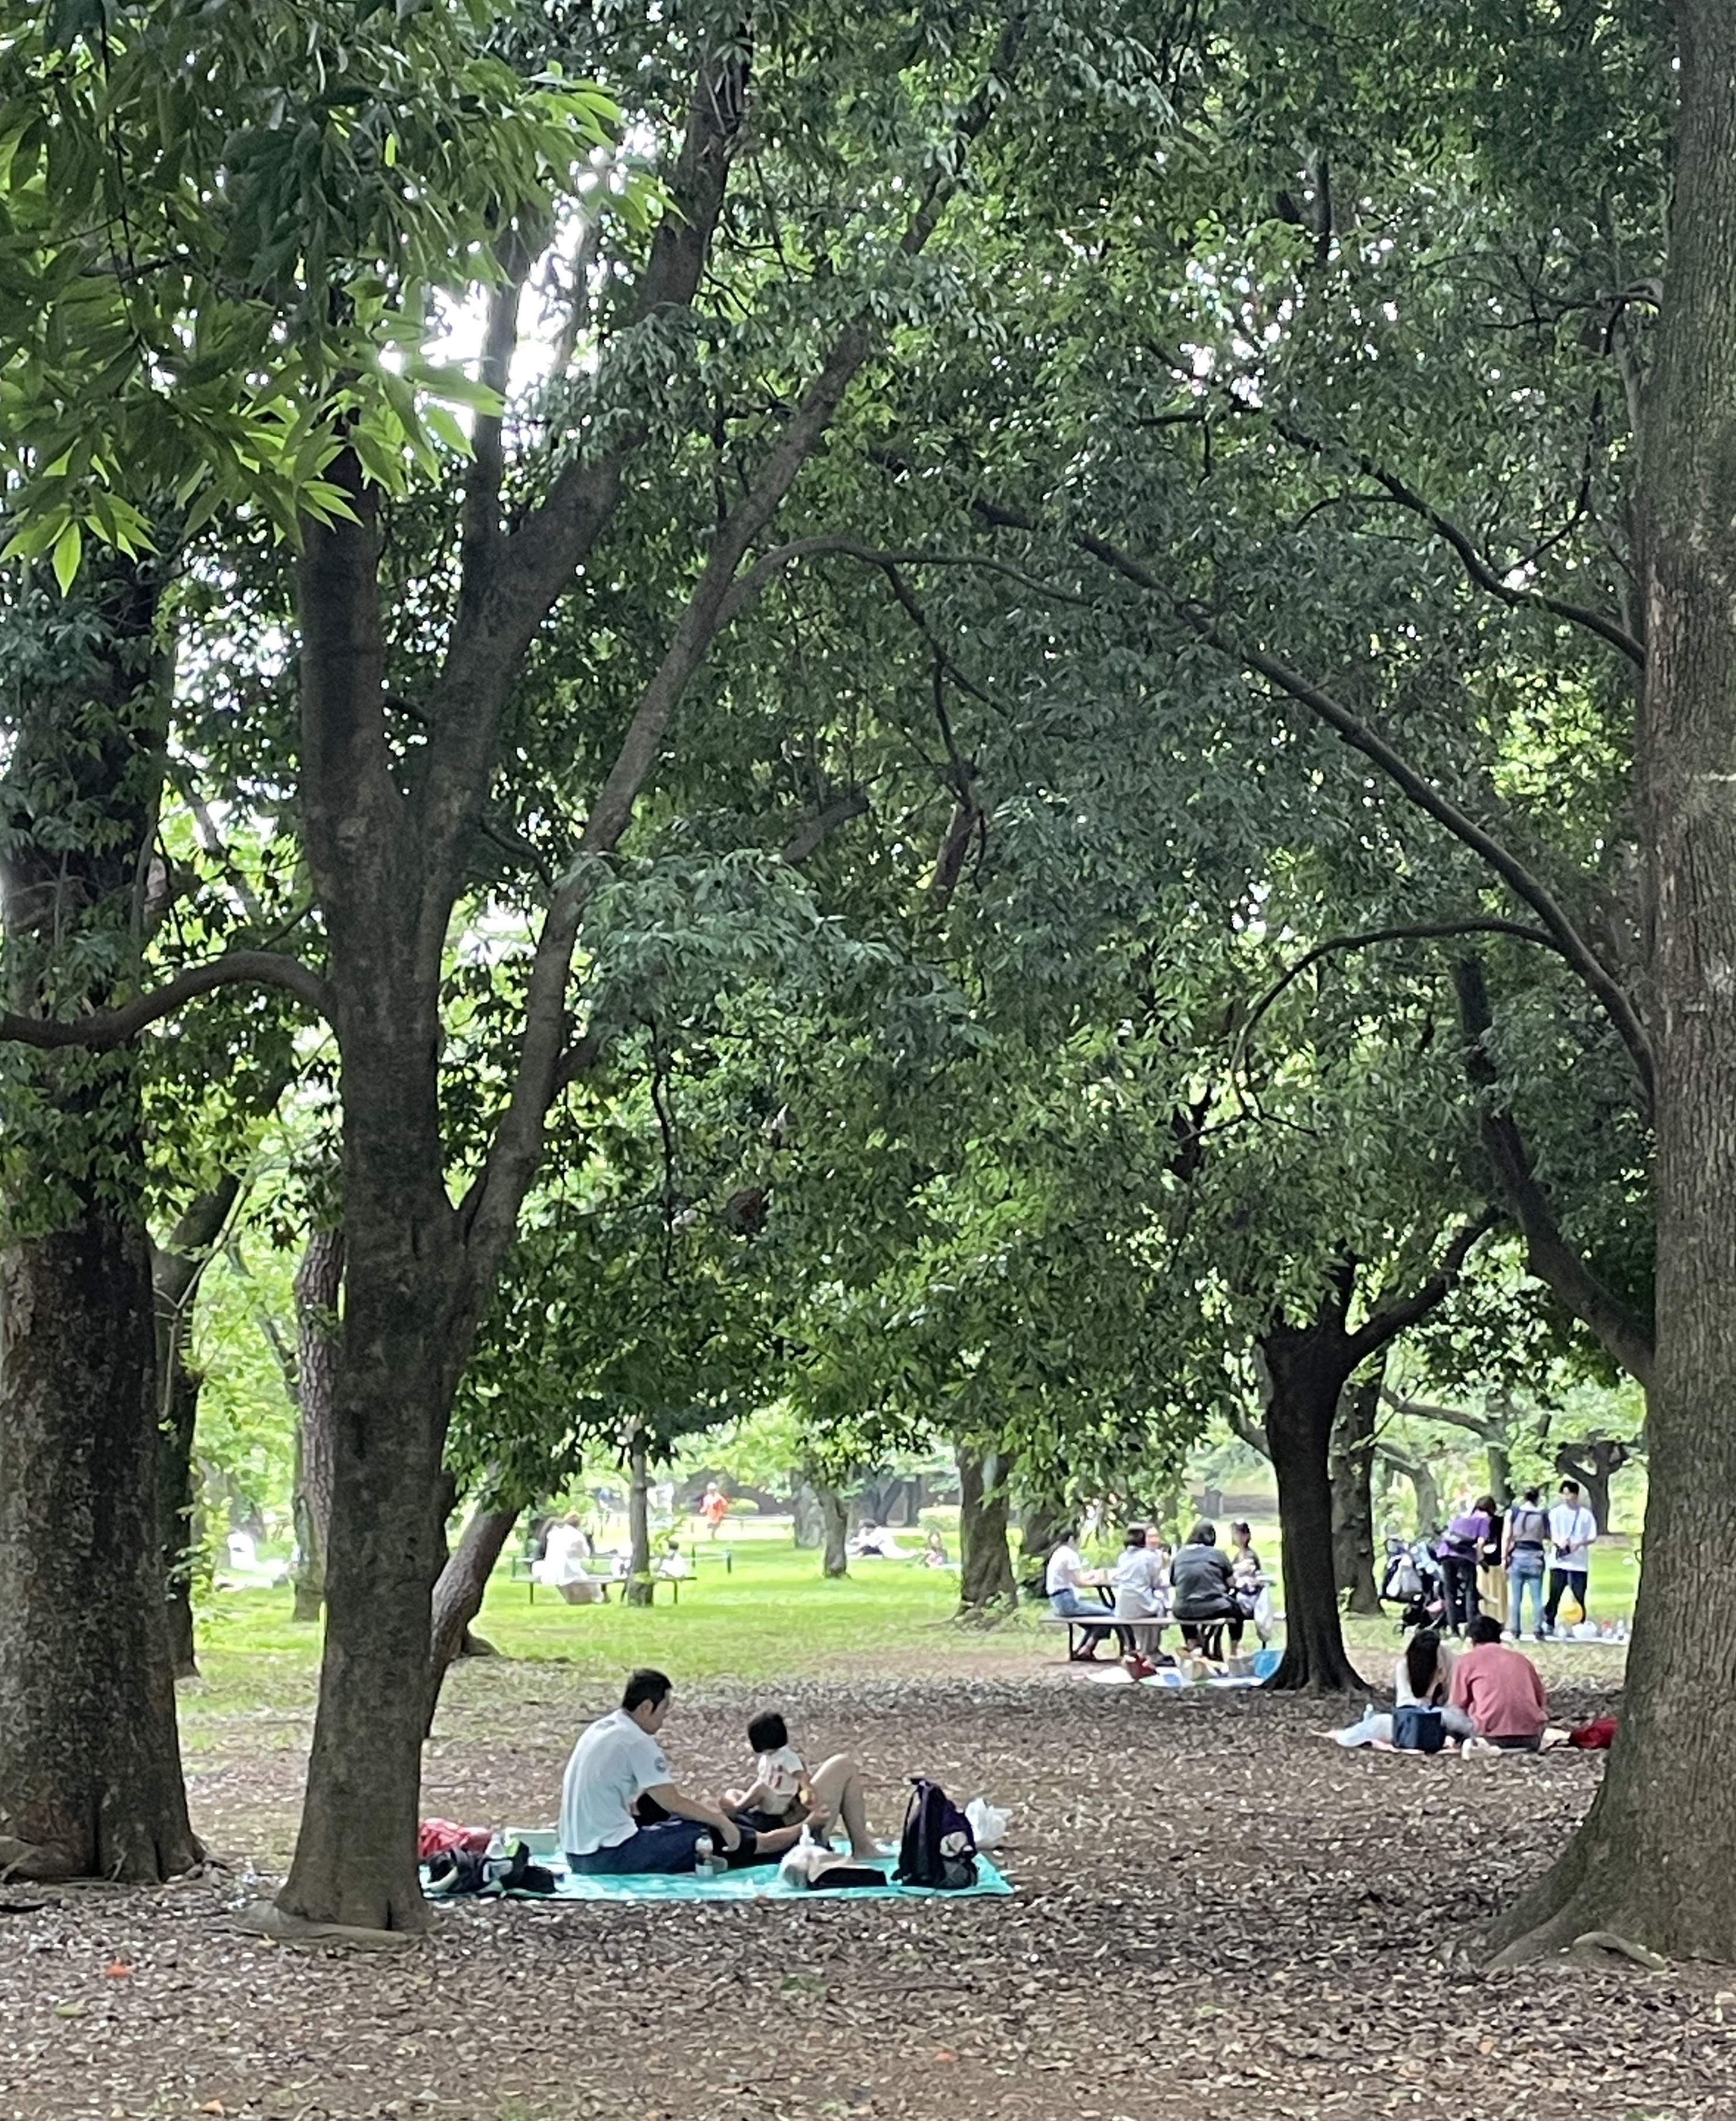
\includegraphics[width=\linewidth]{images/gatherings/yoyogi_trees_image1.jpeg}\par\hspace{0.5pt}
    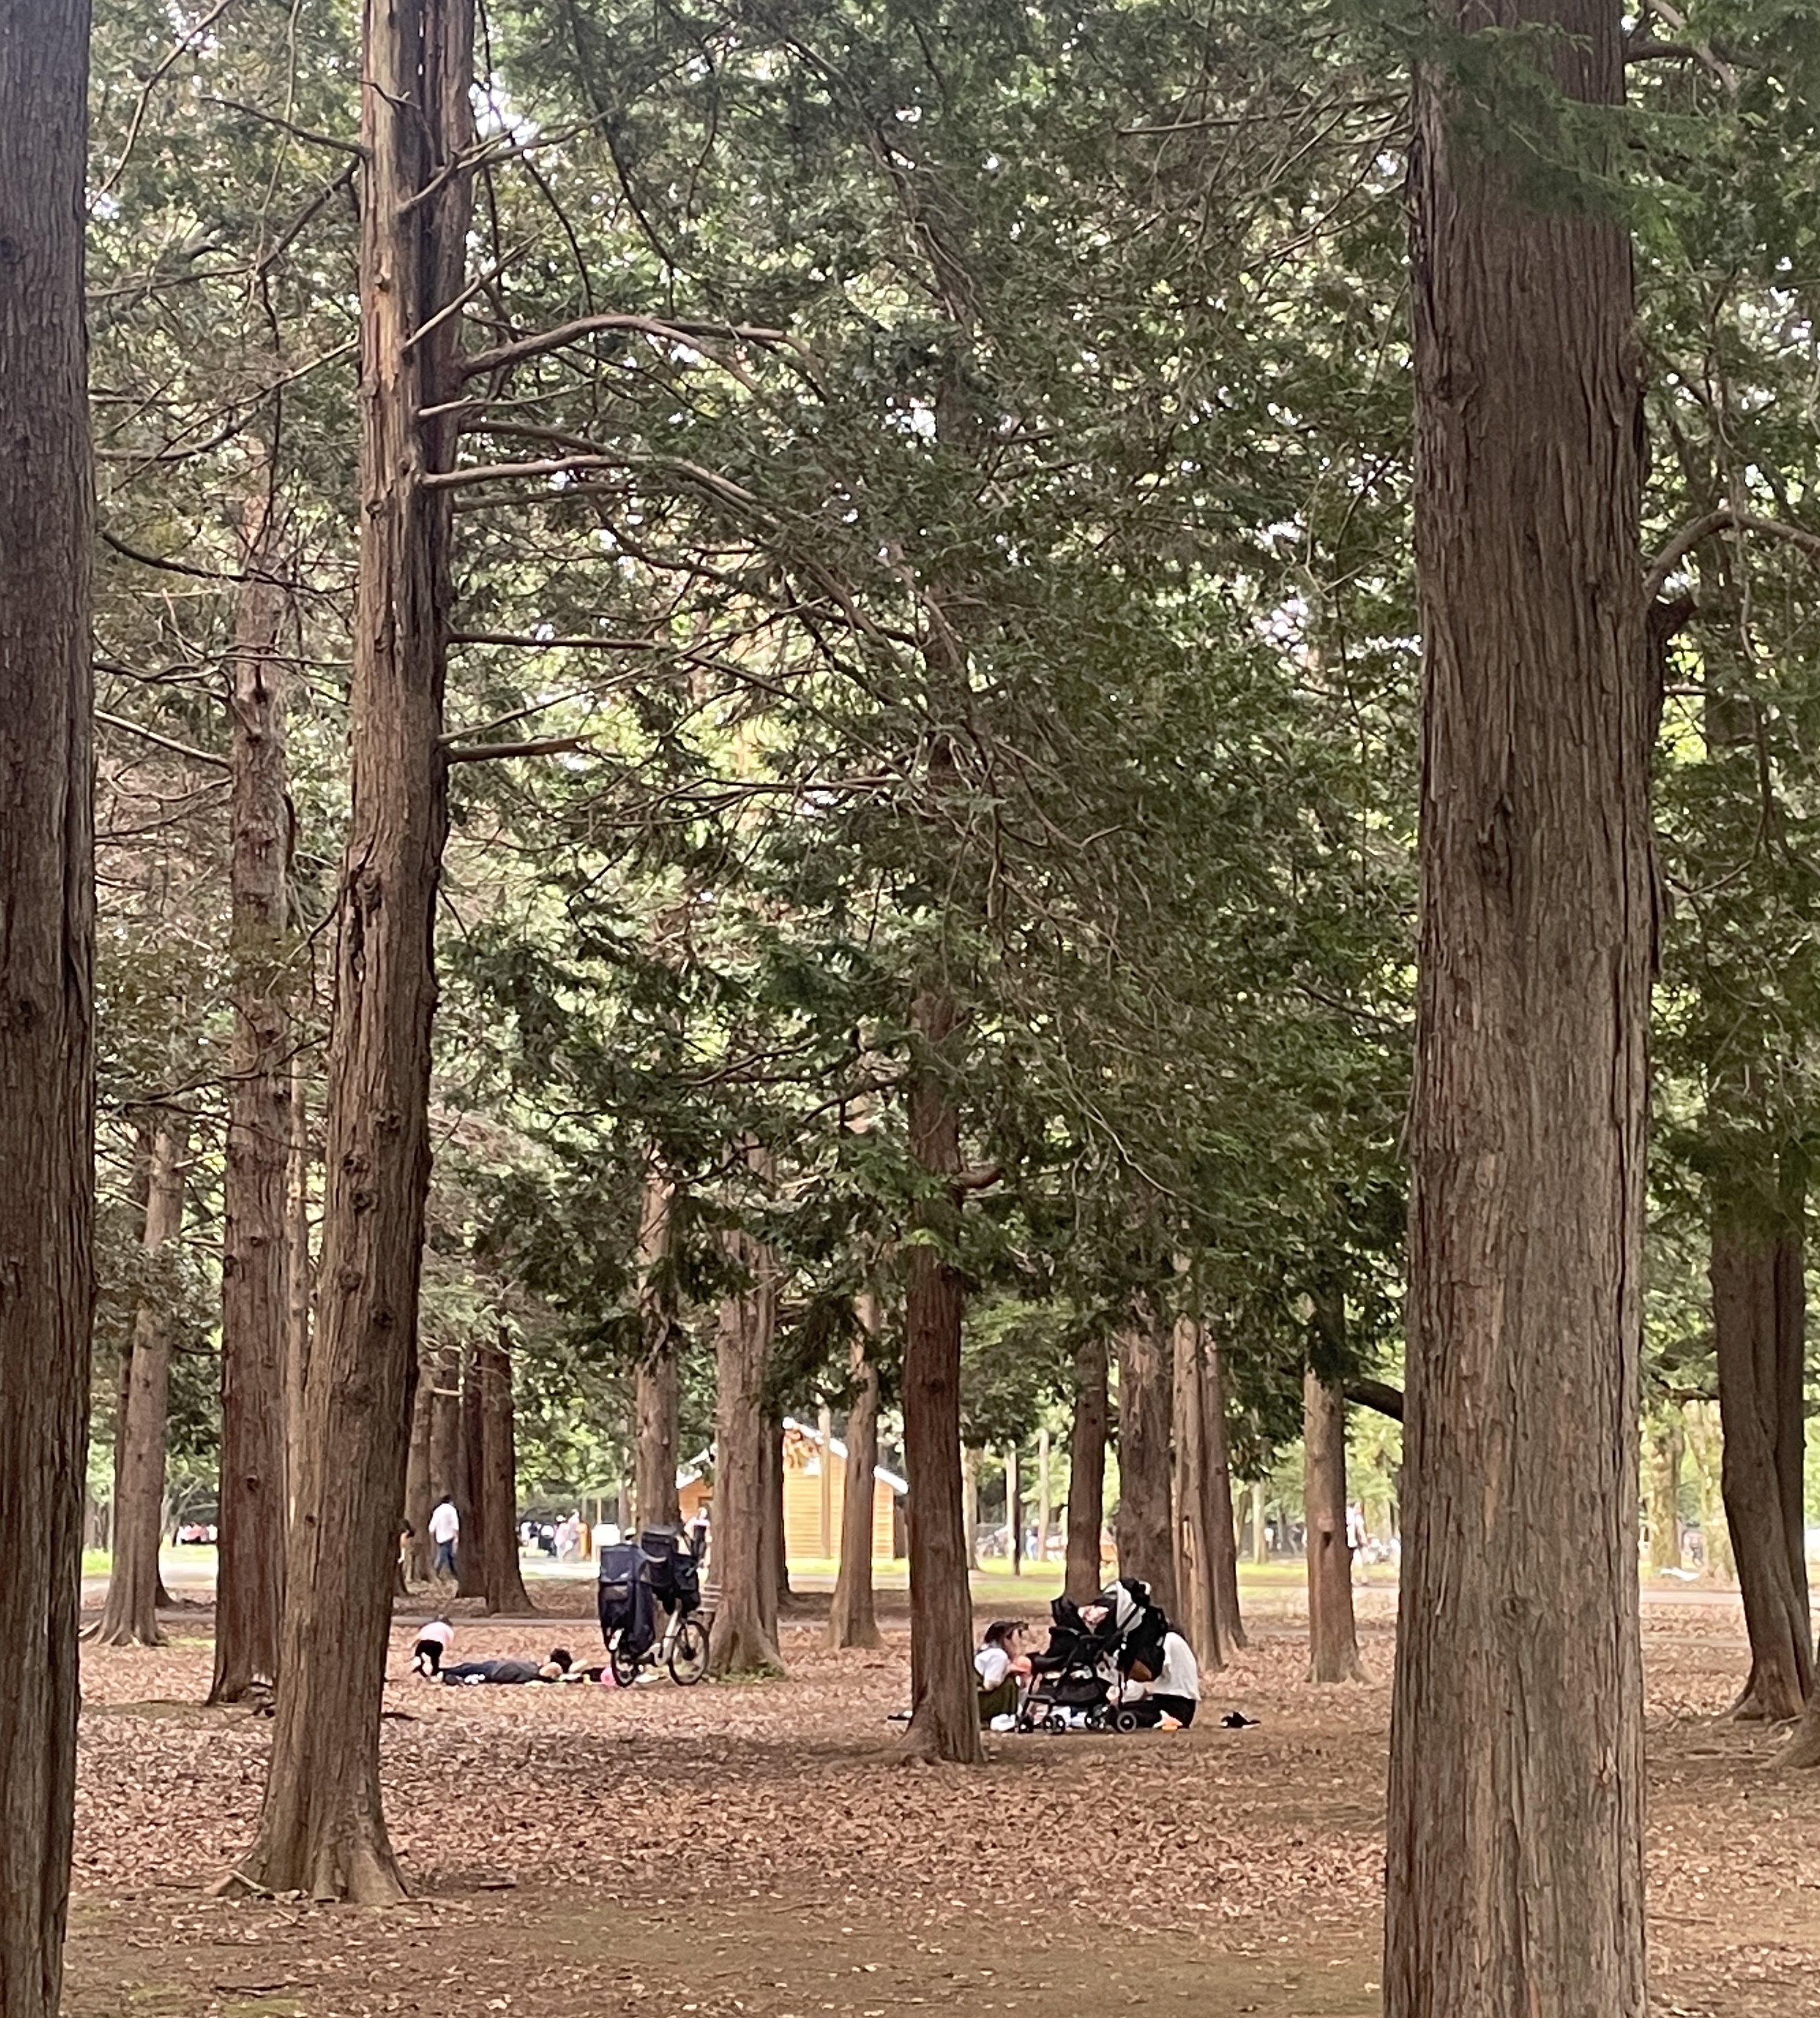
\includegraphics[width=\linewidth]{images/gatherings/yoyogi_trees_image2.jpeg}\par\captionof{figure}[Yoyogi Park images]{Outdoor gatherings under the tree canopy in Yoyogi park, photographs by the author on June 24, 2023.}
    \label{fig:yoyogi_trees_images}\par\hspace{0.5pt}
    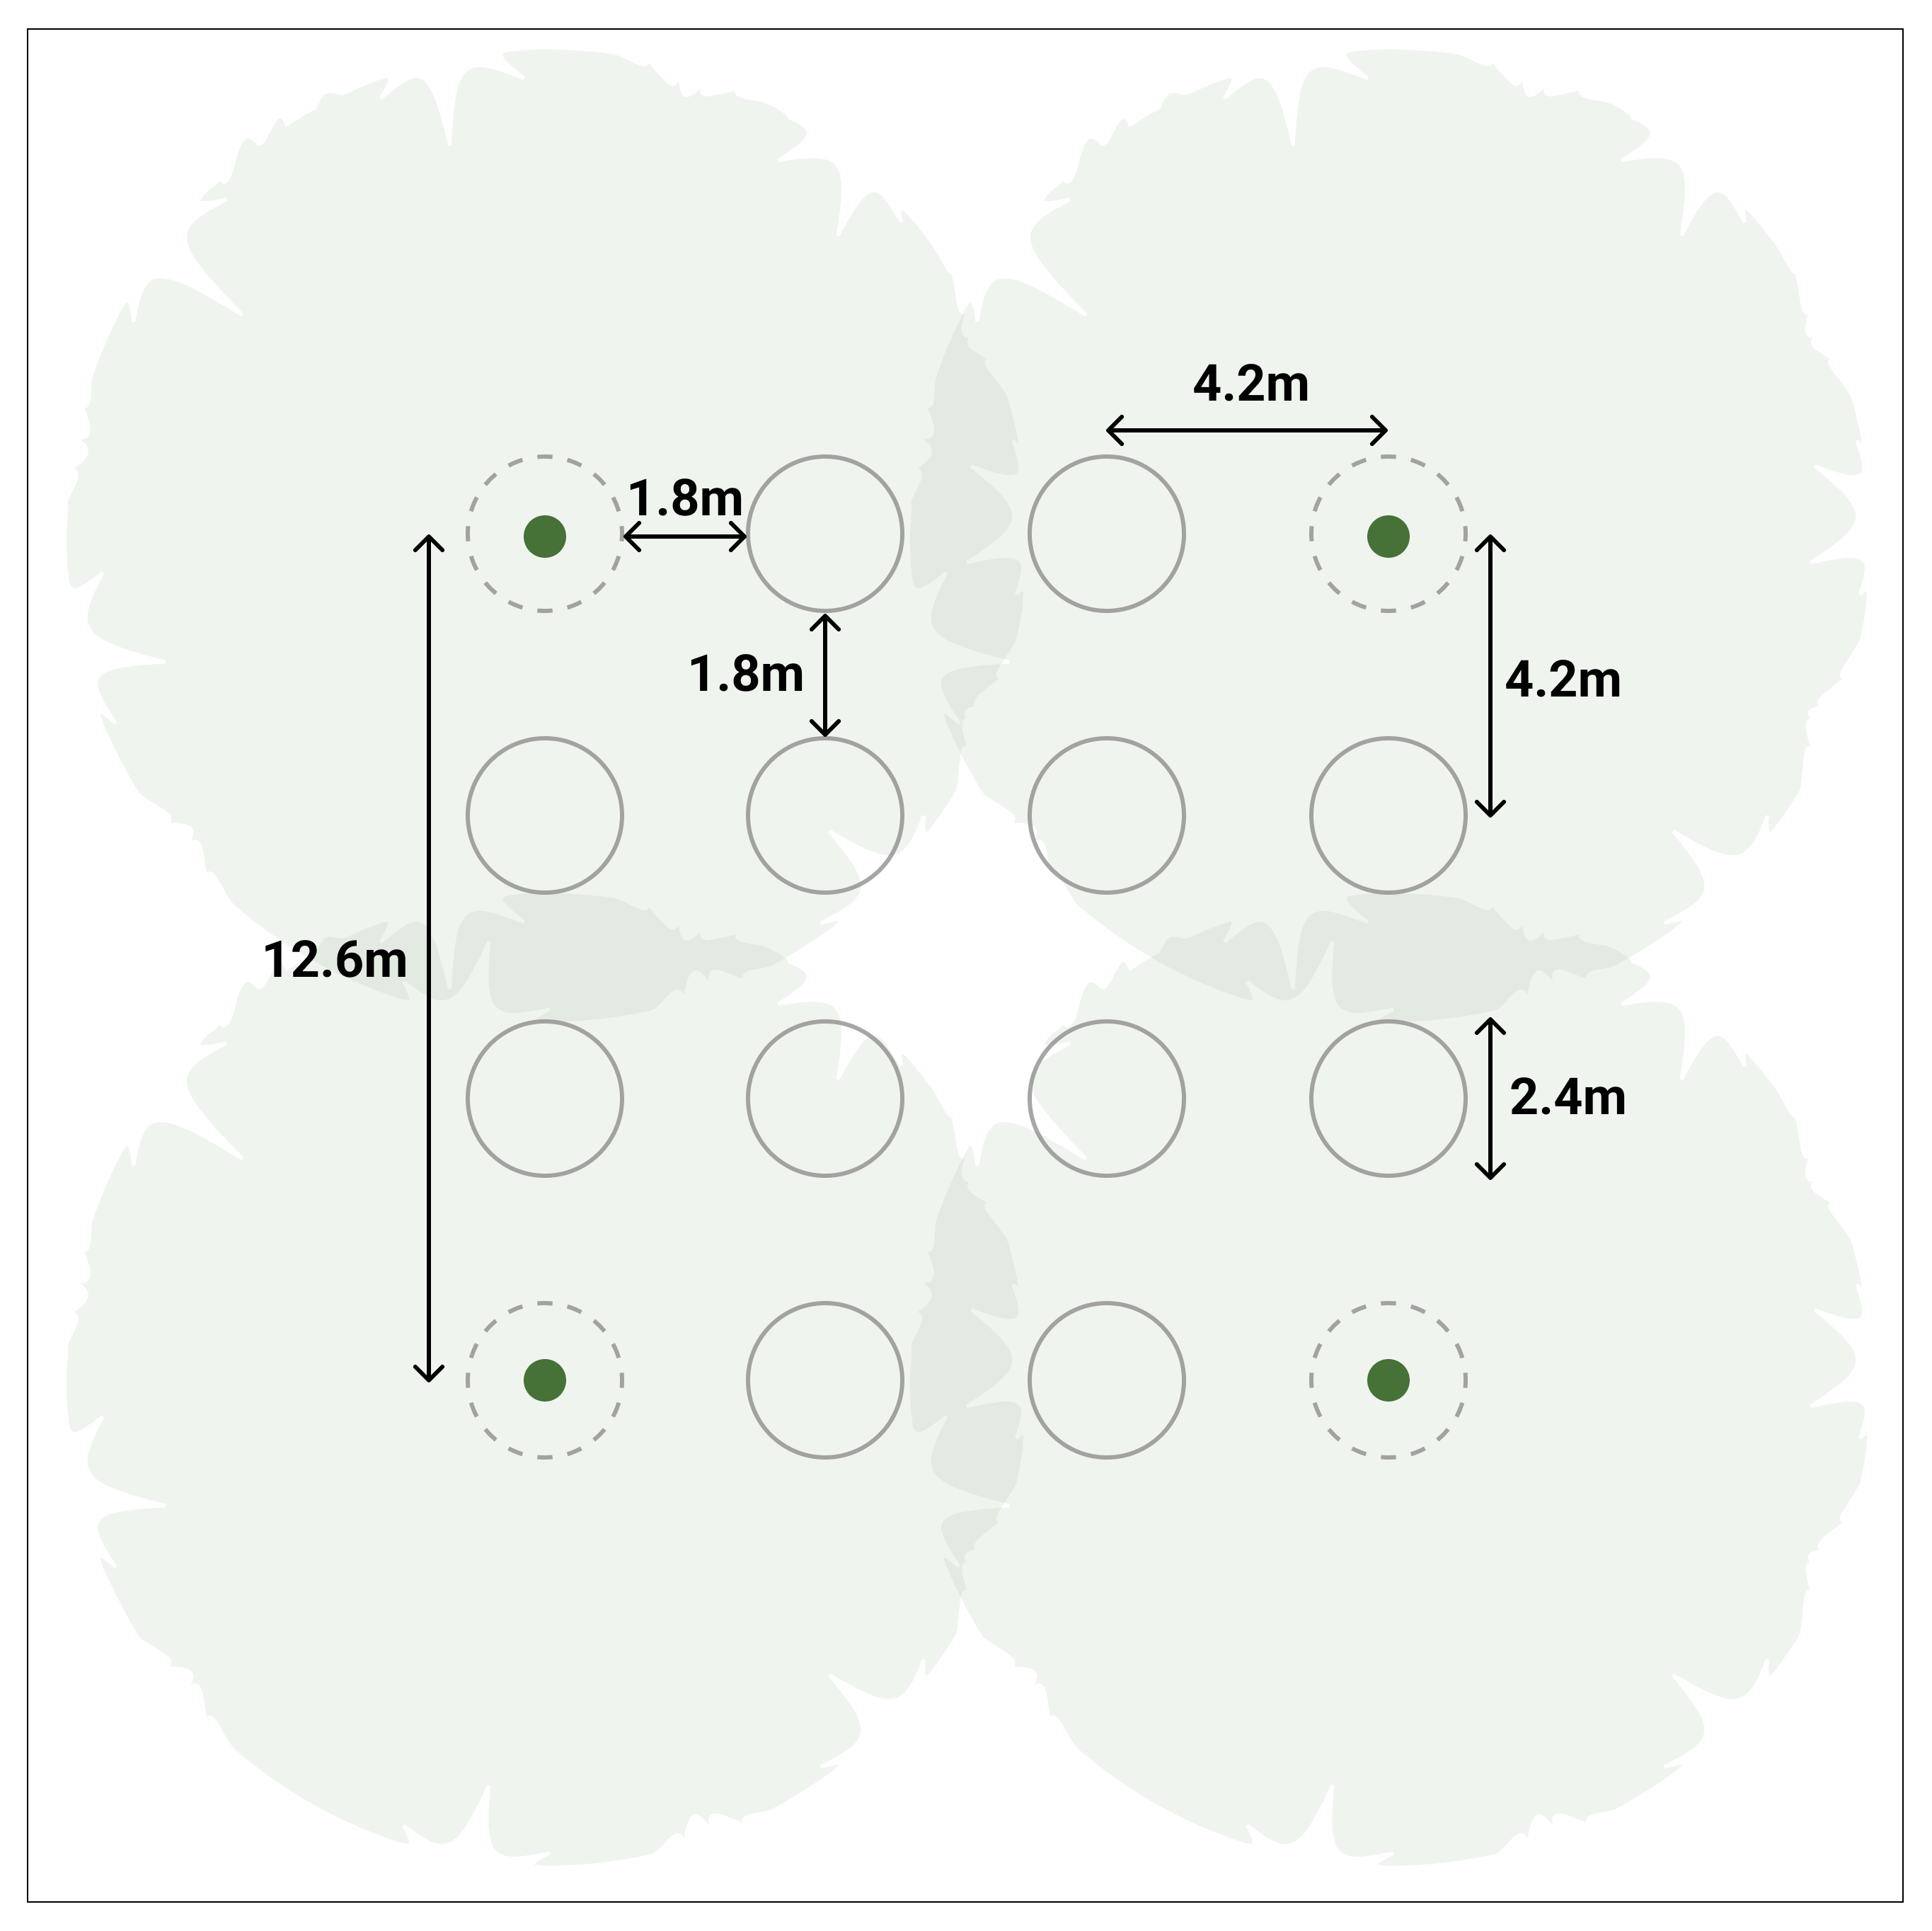
\includegraphics[width=\linewidth]{images/gatherings/yoyogi_trees.png}\par\captionof{figure}[Yoyogi Park tree canopy dimensions]{Diagram of the average dimensions between trees in Yoyogi Park.}
    \label{fig:yoyogi_trees}
\end{minipage}

\end{multicols}

\begin{figure}[h]
  \centering
  \captionsetup{width=1.0\linewidth}
  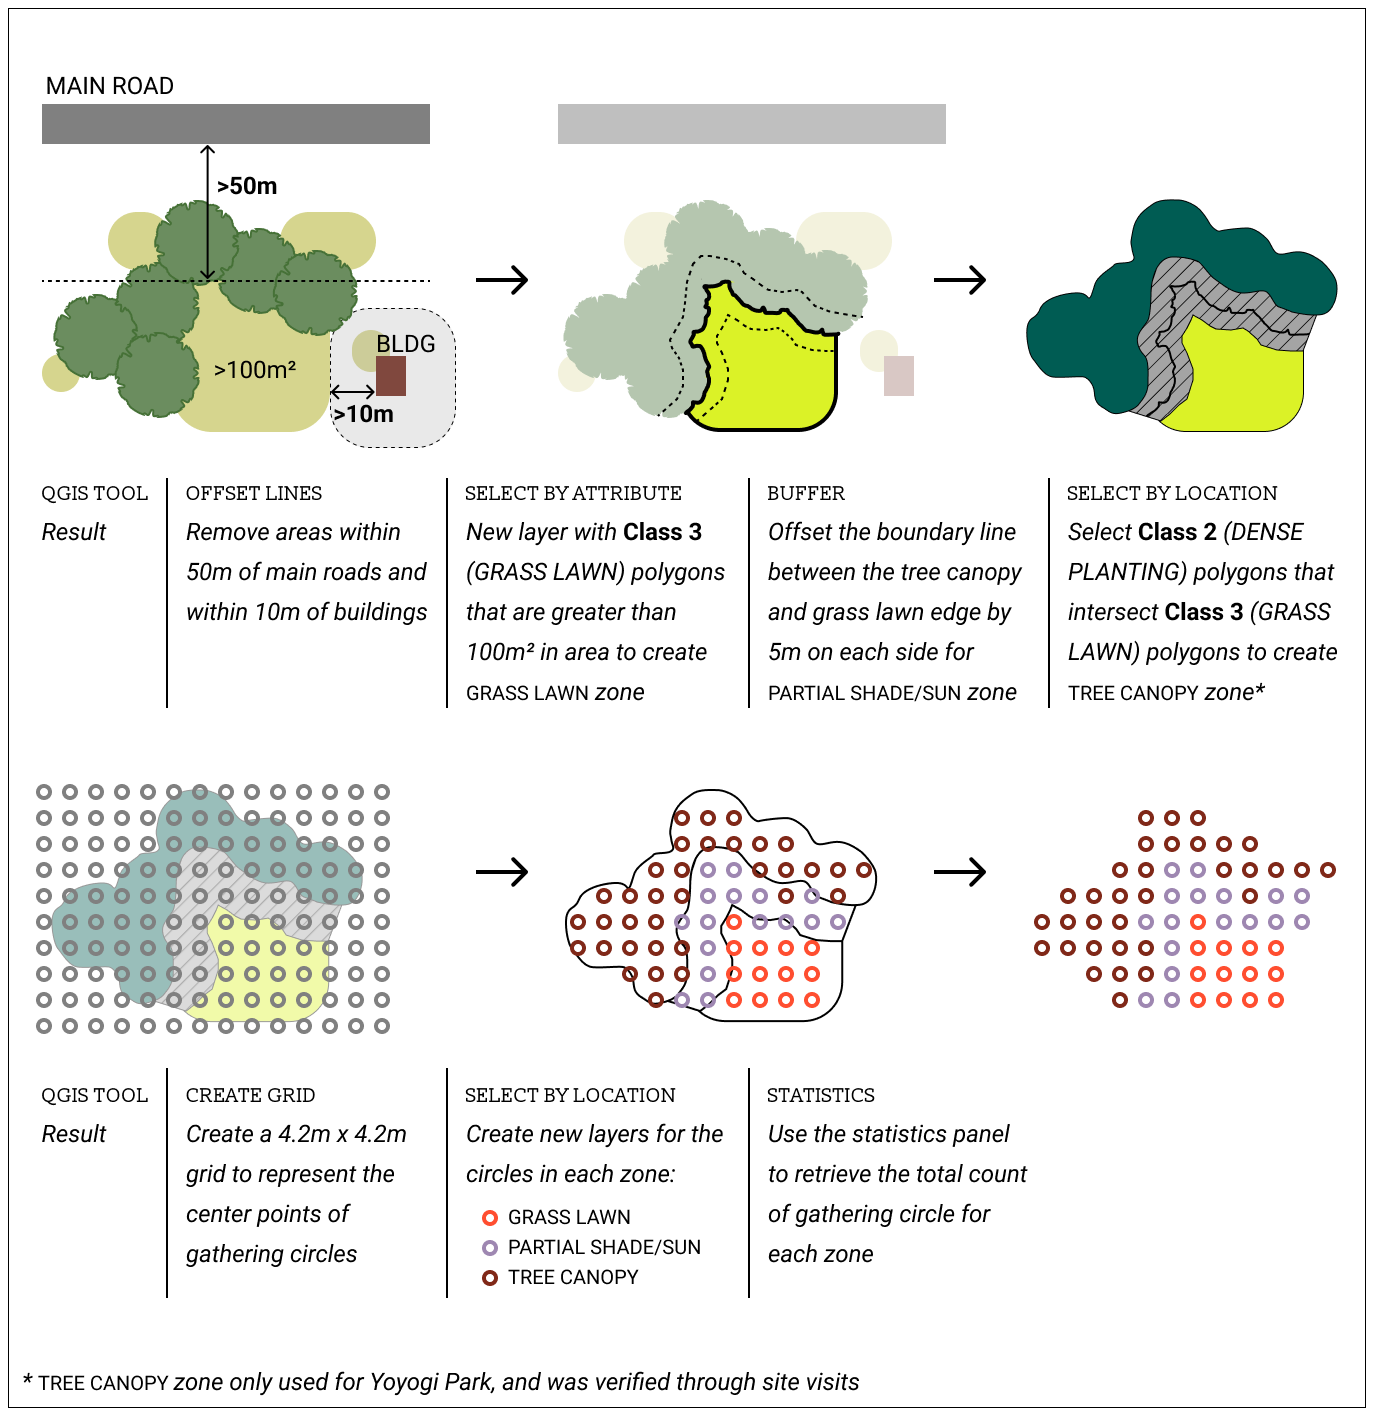
\includegraphics[width=1.0\textwidth]{images/gatherings/quantifying.png}
  \caption[Process diagram]{Explanatory process diagram of using QGIS tools to quantify gathering circles from image classification vector objects.} 
  \label{fig:quantifying}
\end{figure}

\begin{table}[h]
  \centering
\small
\begin{tabular}{lcrcrccc}
\toprule
{} &      Area &  {} &  Partial &  \emph{Tree canopy} &  Adjusted  &  {} &  Percentage\\
Park Name &      $ (km^{2}) $ &  Grass lawn &  shade/sun &  \emph{(not in total)} & tree canopy & Total &  of park\\
\midrule
Hyde Park &      1.40 &     10157 &           6368 &           - &               - &        16525 &     21.12\% \\
Prospect Park &      1.80 &      6806 &           5336 &           - &               - &        12142 &     11.19\% \\
Yoyogi Park &      0.56 &       858 &           3793 &        \emph{7647} &            5735 &        10386 &     32.75\% \\
\bottomrule
\end{tabular}
\caption[Gatherings gount]{Number of gathering circles in each park by sun exposure and thermal comfort.}
\label{gatherings_count}
\end{table}

\begin{multicols}{2}

\section{Quantifying outdoor gatherings}
\subsection{QGIS tools}
The grass lawns identified in the image classification analysis are the starting point for quantifying the number of social gatherings that can occur in each park. Using various QGIS tools, the conditions from Section \ref{conditions} narrow down the areas to those that are protected from the main road, not too close to buildings, and are large enough in area to be considered a space for social activity. Tree canopies identified directly adjacent to those grass lawns are then used to create a partial sun/shade zone by offsetting (using the QGIS 'Buffer' tool) the edge of the canopy by five meters on either side. Once the extents of these two zones are found, the spacing from the Domino Park case study (see Figure \ref{fig:circle_dims}) is used to create a grid representing the gathering circles which fall inside each zone boundary as demonstrated in Figure \ref{fig:quantifying}.

\subsection{Results}
Table \ref{gatherings_count} shows the maximum number of gathering circles that could be located in each zone of each park. Gathering circles under the tree canopy are not identified for Hyde Park and Prospect Park due to the climatic conditions and cultural preferences described previously. For those two parks, it is assumed that visitors who prefer the shade will make use of the partial sun/shade zone identified in this study. Regarding the tree canopy zone for Yoyogi Park, it was discovered from site visits that the trees are spaced fairly regularly, with roughly one tree every 12 meters. As shown in Figure \ref{fig:yoyogi_trees}, for every sixteen social gathering circles about four of those circles will likely be obstructed by tree trunks and the surrounding roots. The "Adjusted tree canopy" column in Table \ref{gatherings_count} shows the values found for the number of gathering circles under tree canopies is adjusted to remove 25\% of the circles to account for this condition. 

The "percentage of park" column is calculated by populating the entire park with the gathering circle grid, then comparing the sum of gathering circles in the three zones to the number of circles that would fit in the entire park. Although Yoyogi Park is significantly smaller than Hyde Park and Prospect Park, the conditions allowing for tree canopy gatherings create the opportunity for more than 5700 circles, which is more than the grass lawn and partial shade/sun spaces combined for Yoyogi Park. Using this criteria, Yoyogi Park has the largest number of gathering spaces per total park area, with 32.75\% of the park being usable for social gatherings. Prospect Park, meanwhile, has the lowest percentage of gathering spaces compared to the total park capacity at 11.19\%. This could be due to the variety of other program and physical features of the park including a zoo, sports centers, and large water features than consume more than 10\% of the park area (see Table \ref{table:OBIA}).

Moreover, while Hyde Park and Prospect Park were designed to replicate pastoral land in the urban environment, Yoyogi Park was designed to be a "forest park" \cite{cranz_politics_1989} \cite{fuse__1994}. This further explains the large difference in quantity of grass lawn gathering spaces. For example, Hyde Park contains over 10,000 circles in this zone while Yoyogi Park has less than 900 (see Table \ref{gatherings_count}). Whether it was by coincidence or intentionally designed this way is unknown, but the respective designs allow the parks to make use of the land for social gatherings in a way that meets the demand of the local climate (more spaces in the sun for London and shade for Tokyo). 

Figure \ref{fig:hyde_gathering} - \ref{fig:yoyogi_gathering} shows the social gathering zones (grass lawn and partial sun/shade, and tree canopy for Yoyogi Park) as well as the distribution of gathering circles (see Figure \ref{fig:gathering_legend}). Although Prospect Park has the largest area of the three parks, it is evident from the visualizations that the amount of space dedicated to gathering circles is noticeably less than that of the other two parks. Figures \ref{fig:locations_1000} and \ref{fig:circles_1000} shows the zoning and gathering circles for the three parks at a larger scale. 

Finally, each circle provides space for one to four individuals to have a social gathering. Therefore, if every gathering circle is filled to capacity, the number of people the park could hold would be four times the number listed in the "Total" column of Table \ref{gatherings_count}. In the next chapter, the total number of social gathering circles in each park will be compared to the population living around the park. 

\begin{minipage}{0.45\textwidth}
    \centering
    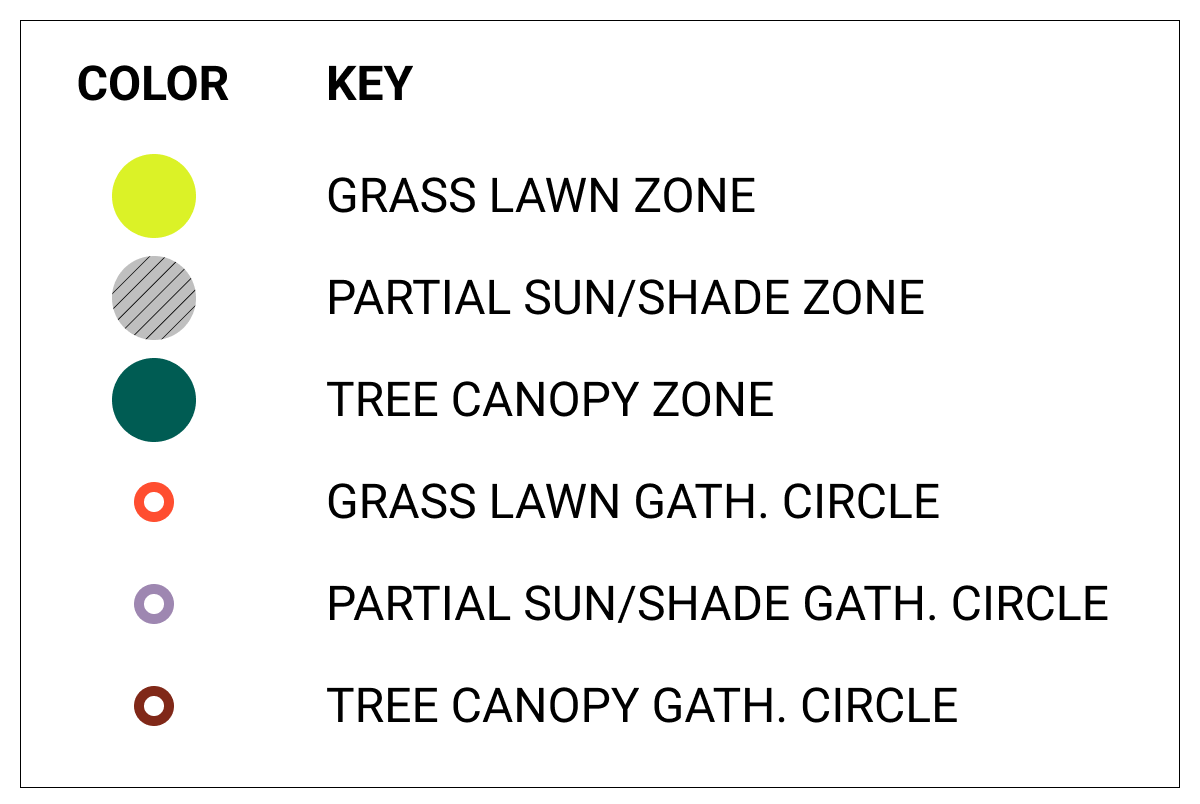
\includegraphics[width=\linewidth]{images/gatherings/gatherings_legend.png}\par\captionof{figure}[Gathering analysis legend]{Gathering analysis legend}
    \label{fig:gathering_legend}
\end{minipage}

\end{multicols}

\begin{figure}[H]
  \centering
  \captionsetup{width=0.9\textwidth}
  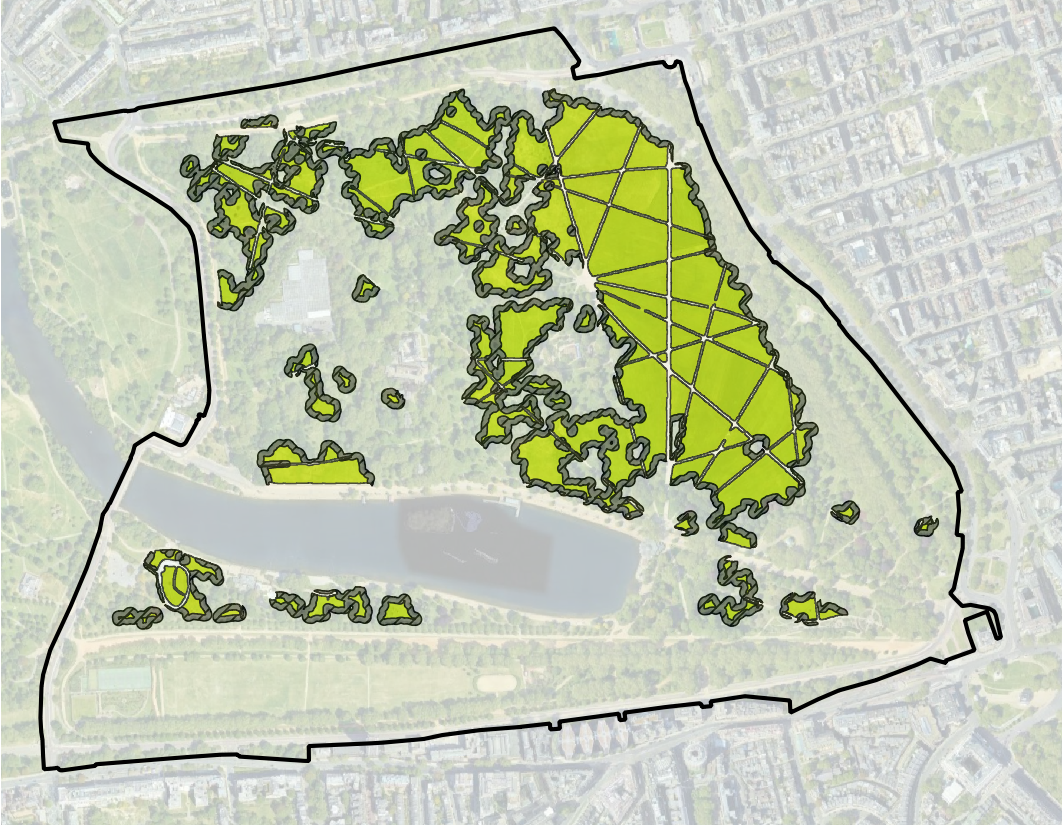
\includegraphics[width=0.9\textwidth]{images/gatherings/hyde_locations.png} \\
  \vspace{10pt}
  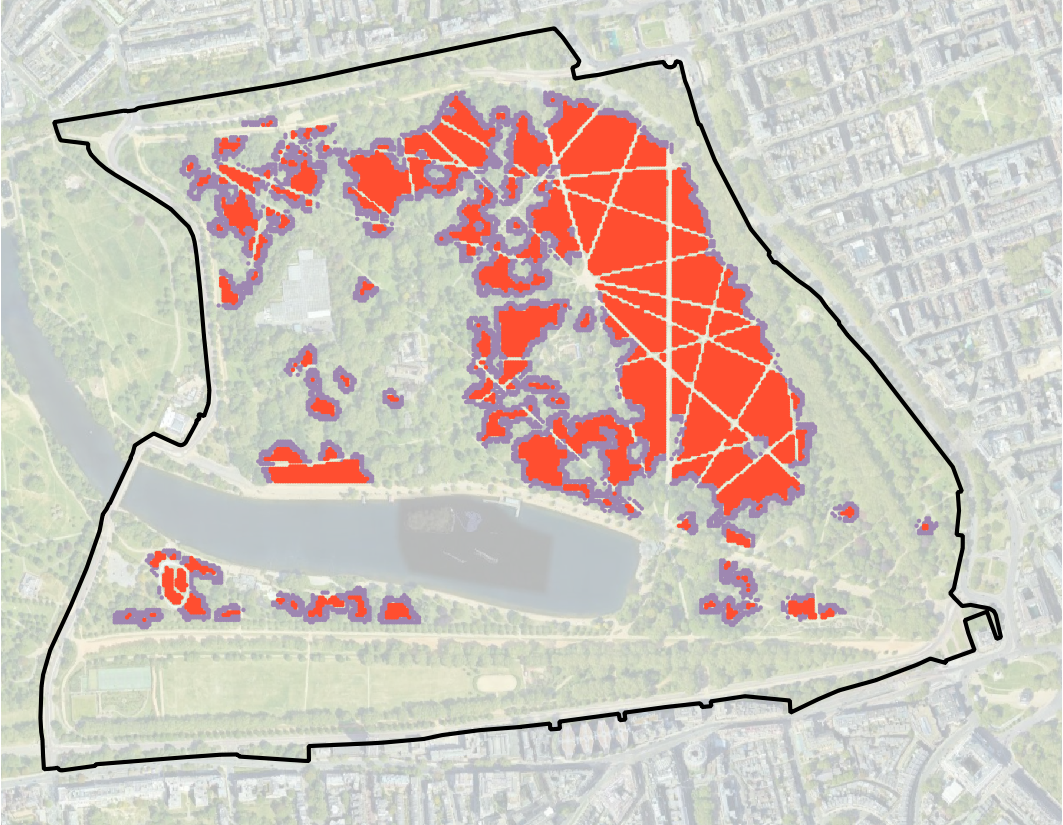
\includegraphics[width=0.9\textwidth]{images/gatherings/hyde_circles.png} \\
  \vspace{10pt}
  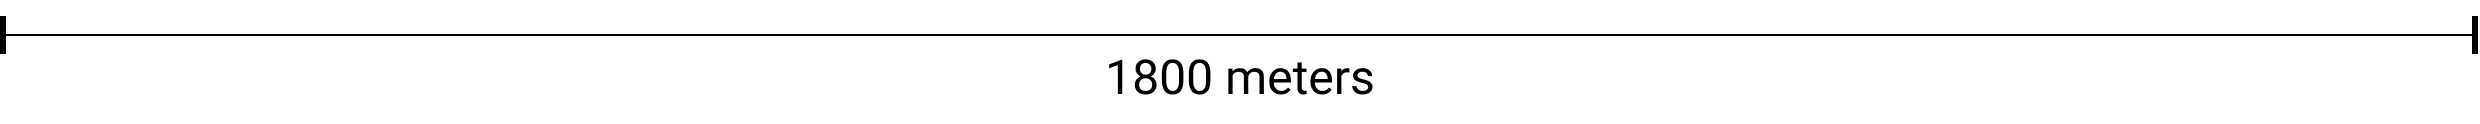
\includegraphics[width=0.9\textwidth]{images/gatherings/scale_legend_2.png}
  \caption[Hyde Park - gathering zones and circles]{Gathering zones and circles by zone in the sun (grass lawn) and partial sun/shade in Hyde Park.}
  \label{fig:hyde_gathering}
\end{figure}

\newpage
\null
\vfill
\begin{figure}[H]
  \centering
  \captionsetup{width=0.9\textwidth}
  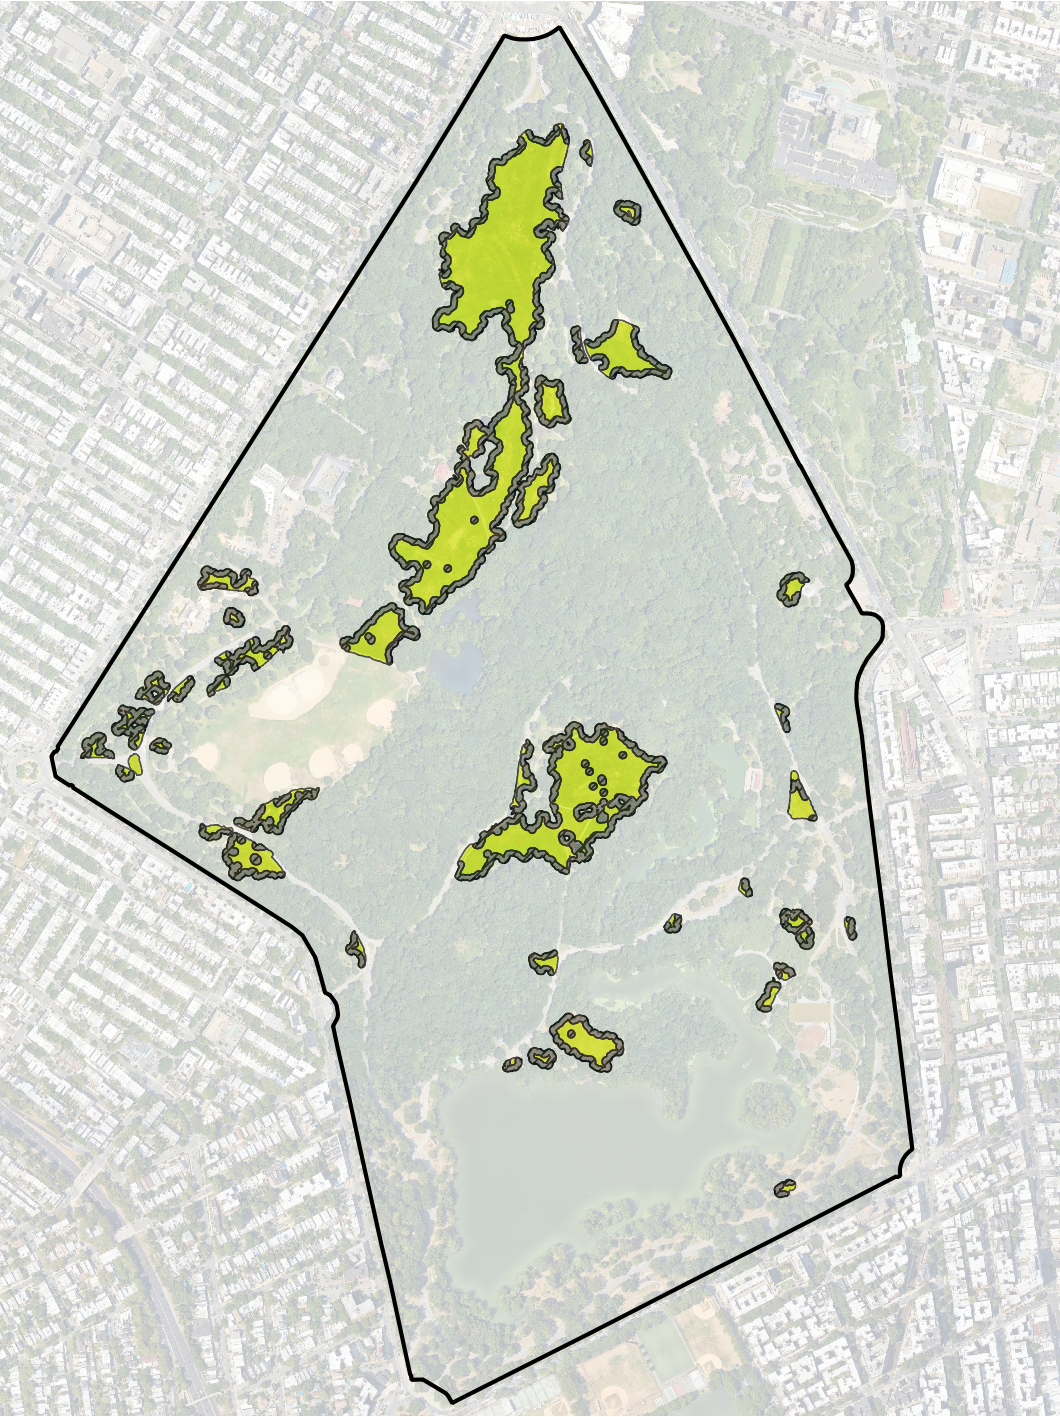
\includegraphics[width=0.9\textwidth]{images/gatherings/prospect_locations.png} \\
  \vspace{10pt}
  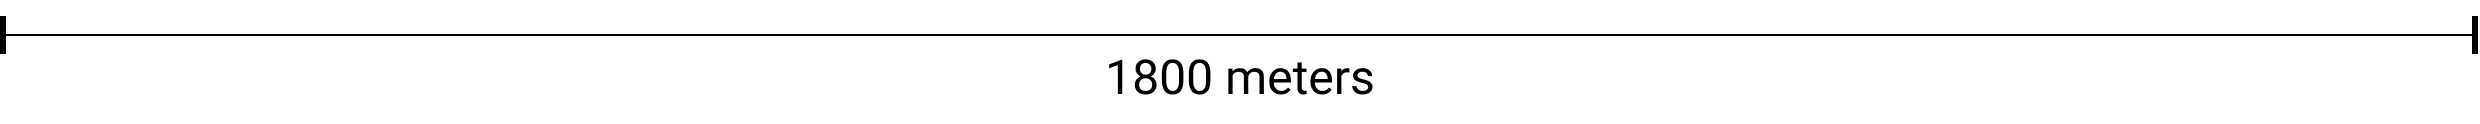
\includegraphics[width=0.9\textwidth]{images/gatherings/scale_legend_2.png}
  \caption[Prospect Park - gathering zones]{Gathering zones in the sun (grass lawn) and partial sun/shade in Prospect Park.}
  \label{fig:prospect_gathering}
\end{figure}

\newpage
\null
\vfill
\begin{figure}[H]
  \centering
  \captionsetup{width=0.9\textwidth}
  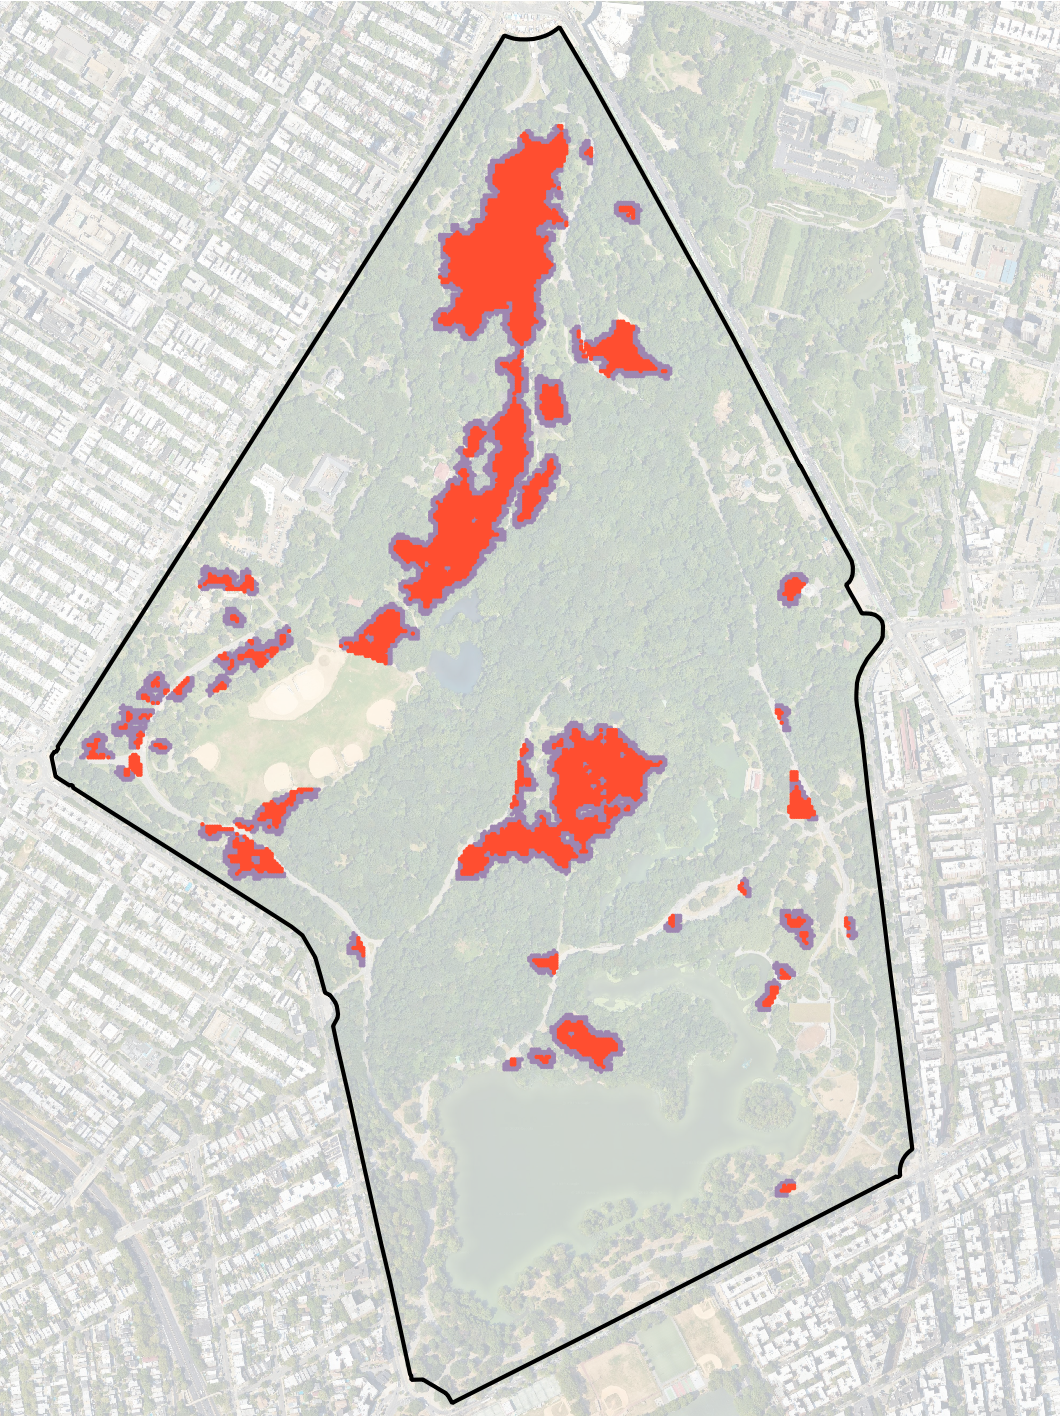
\includegraphics[width=0.9\textwidth]{images/gatherings/prospect_circles.png} \\
  \vspace{10pt}
  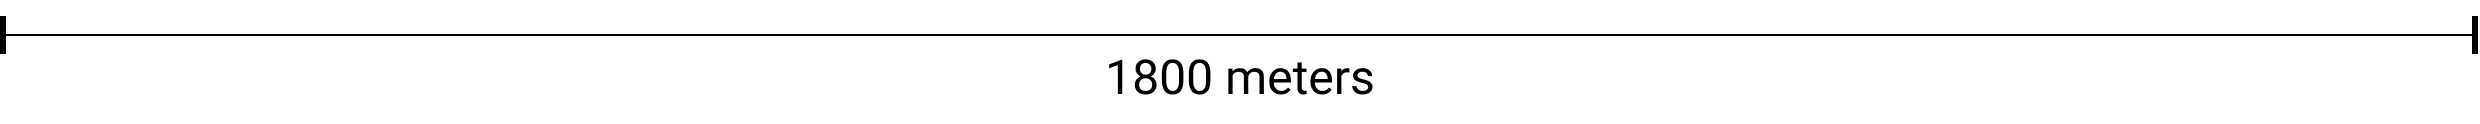
\includegraphics[width=0.9\textwidth]{images/gatherings/scale_legend_2.png}
  \caption[Prospect Park - gathering circles]{Gathering circles by zone in the sun (grass lawn) and partial sun/shade in Prospect Park.}
  \label{fig:prospect_circles}
\end{figure}

\begin{figure}[H]
  \centering
  \captionsetup{width=0.75\textwidth}
  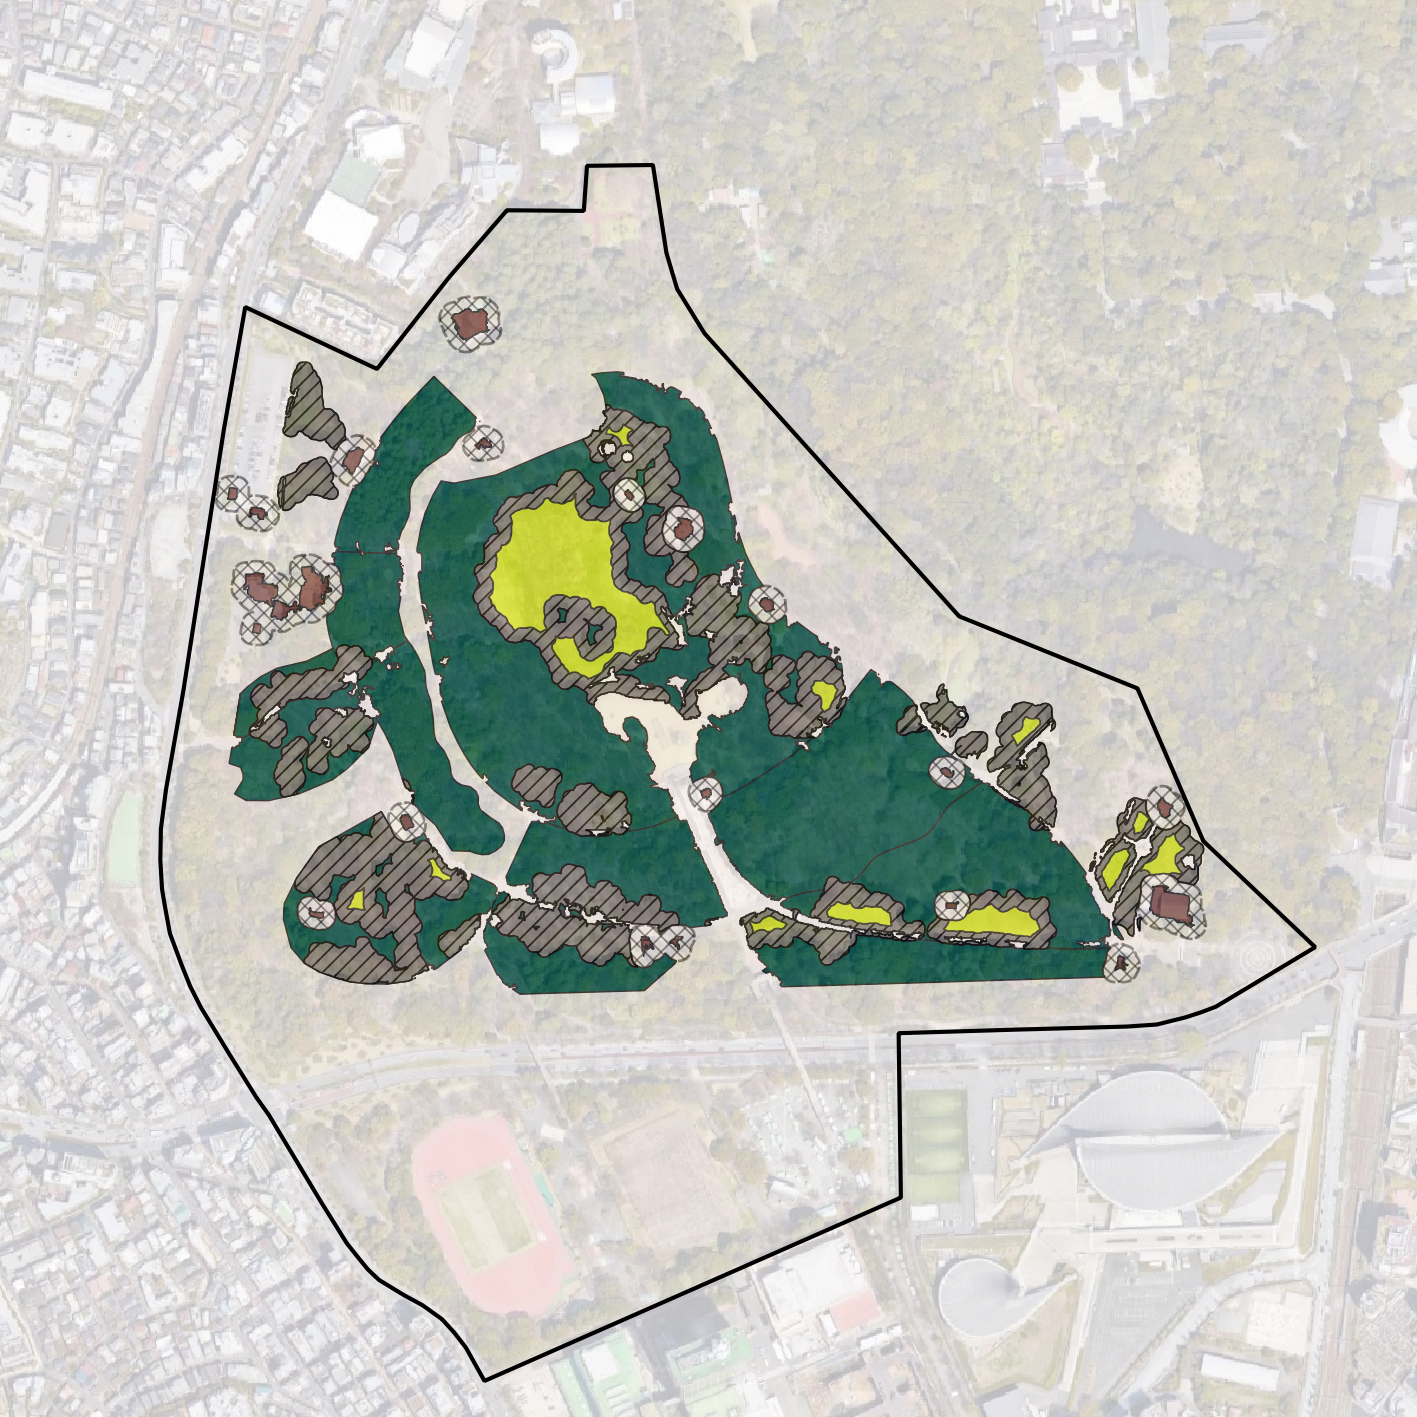
\includegraphics[width=0.75\textwidth]{images/gatherings/yoyogi_locations.png} \\
  \vspace{10pt} % Adjust vertical spacing between the images
  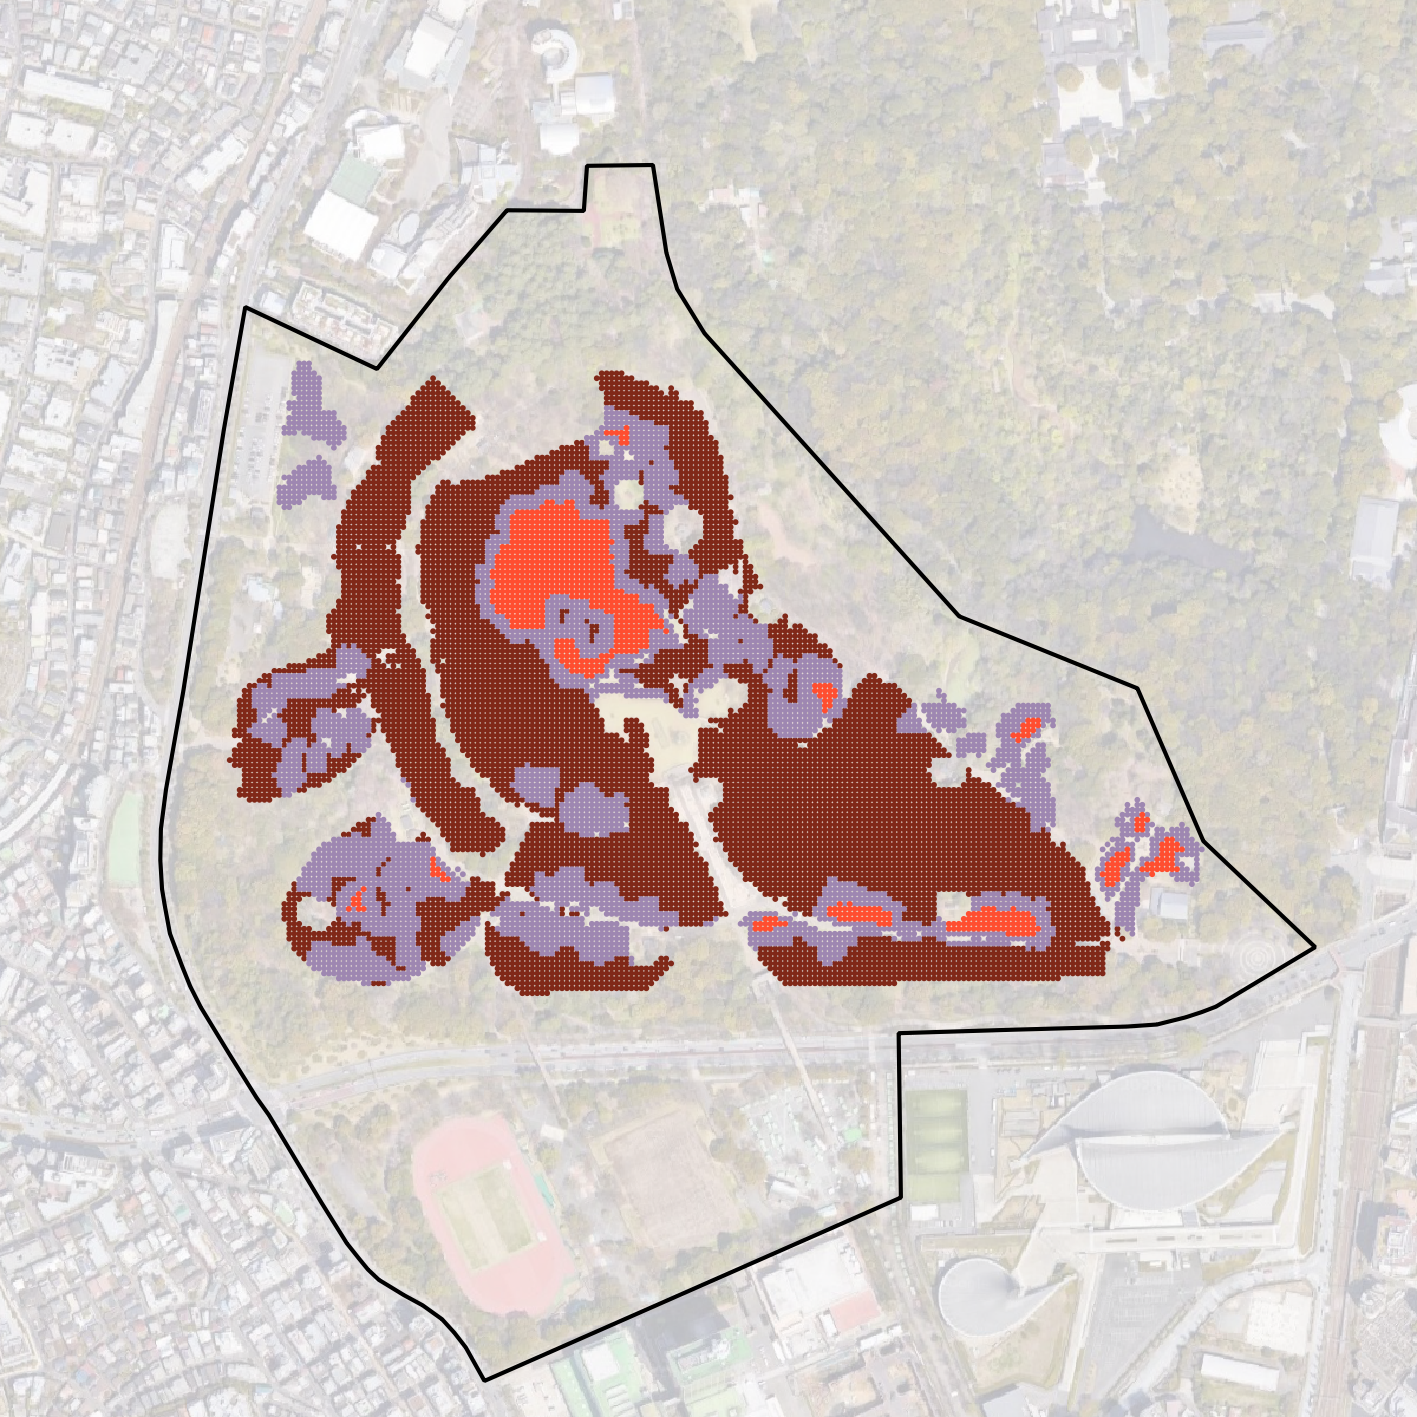
\includegraphics[width=0.75\textwidth]{images/gatherings/yoyogi_circles.png} \\
  \vspace{10pt}
  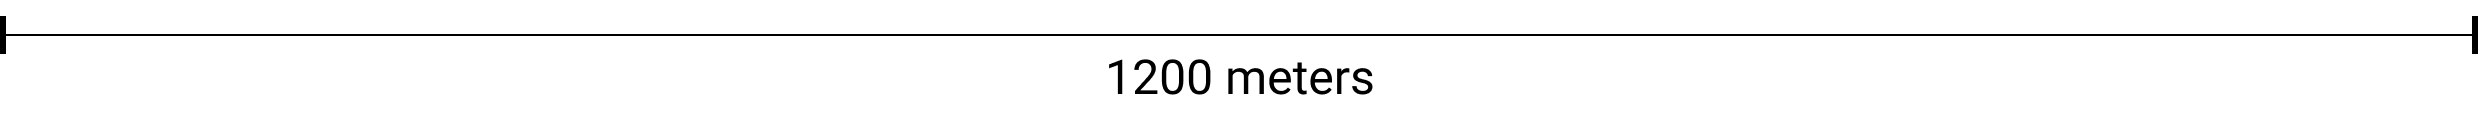
\includegraphics[width=0.75\textwidth]{images/gatherings/scale_legend_3.png}
  \caption[Yoyogi Park - gathering zones and circles]{Gathering zones and circles by zone in the sun (grass lawn), partial sun/shade, and under the tree canopy in Yoyogi Park.}
  \label{fig:yoyogi_gathering}
\end{figure}

\begin{multicols}{2}

\begin{minipage}{0.45\textwidth}
    \centering
    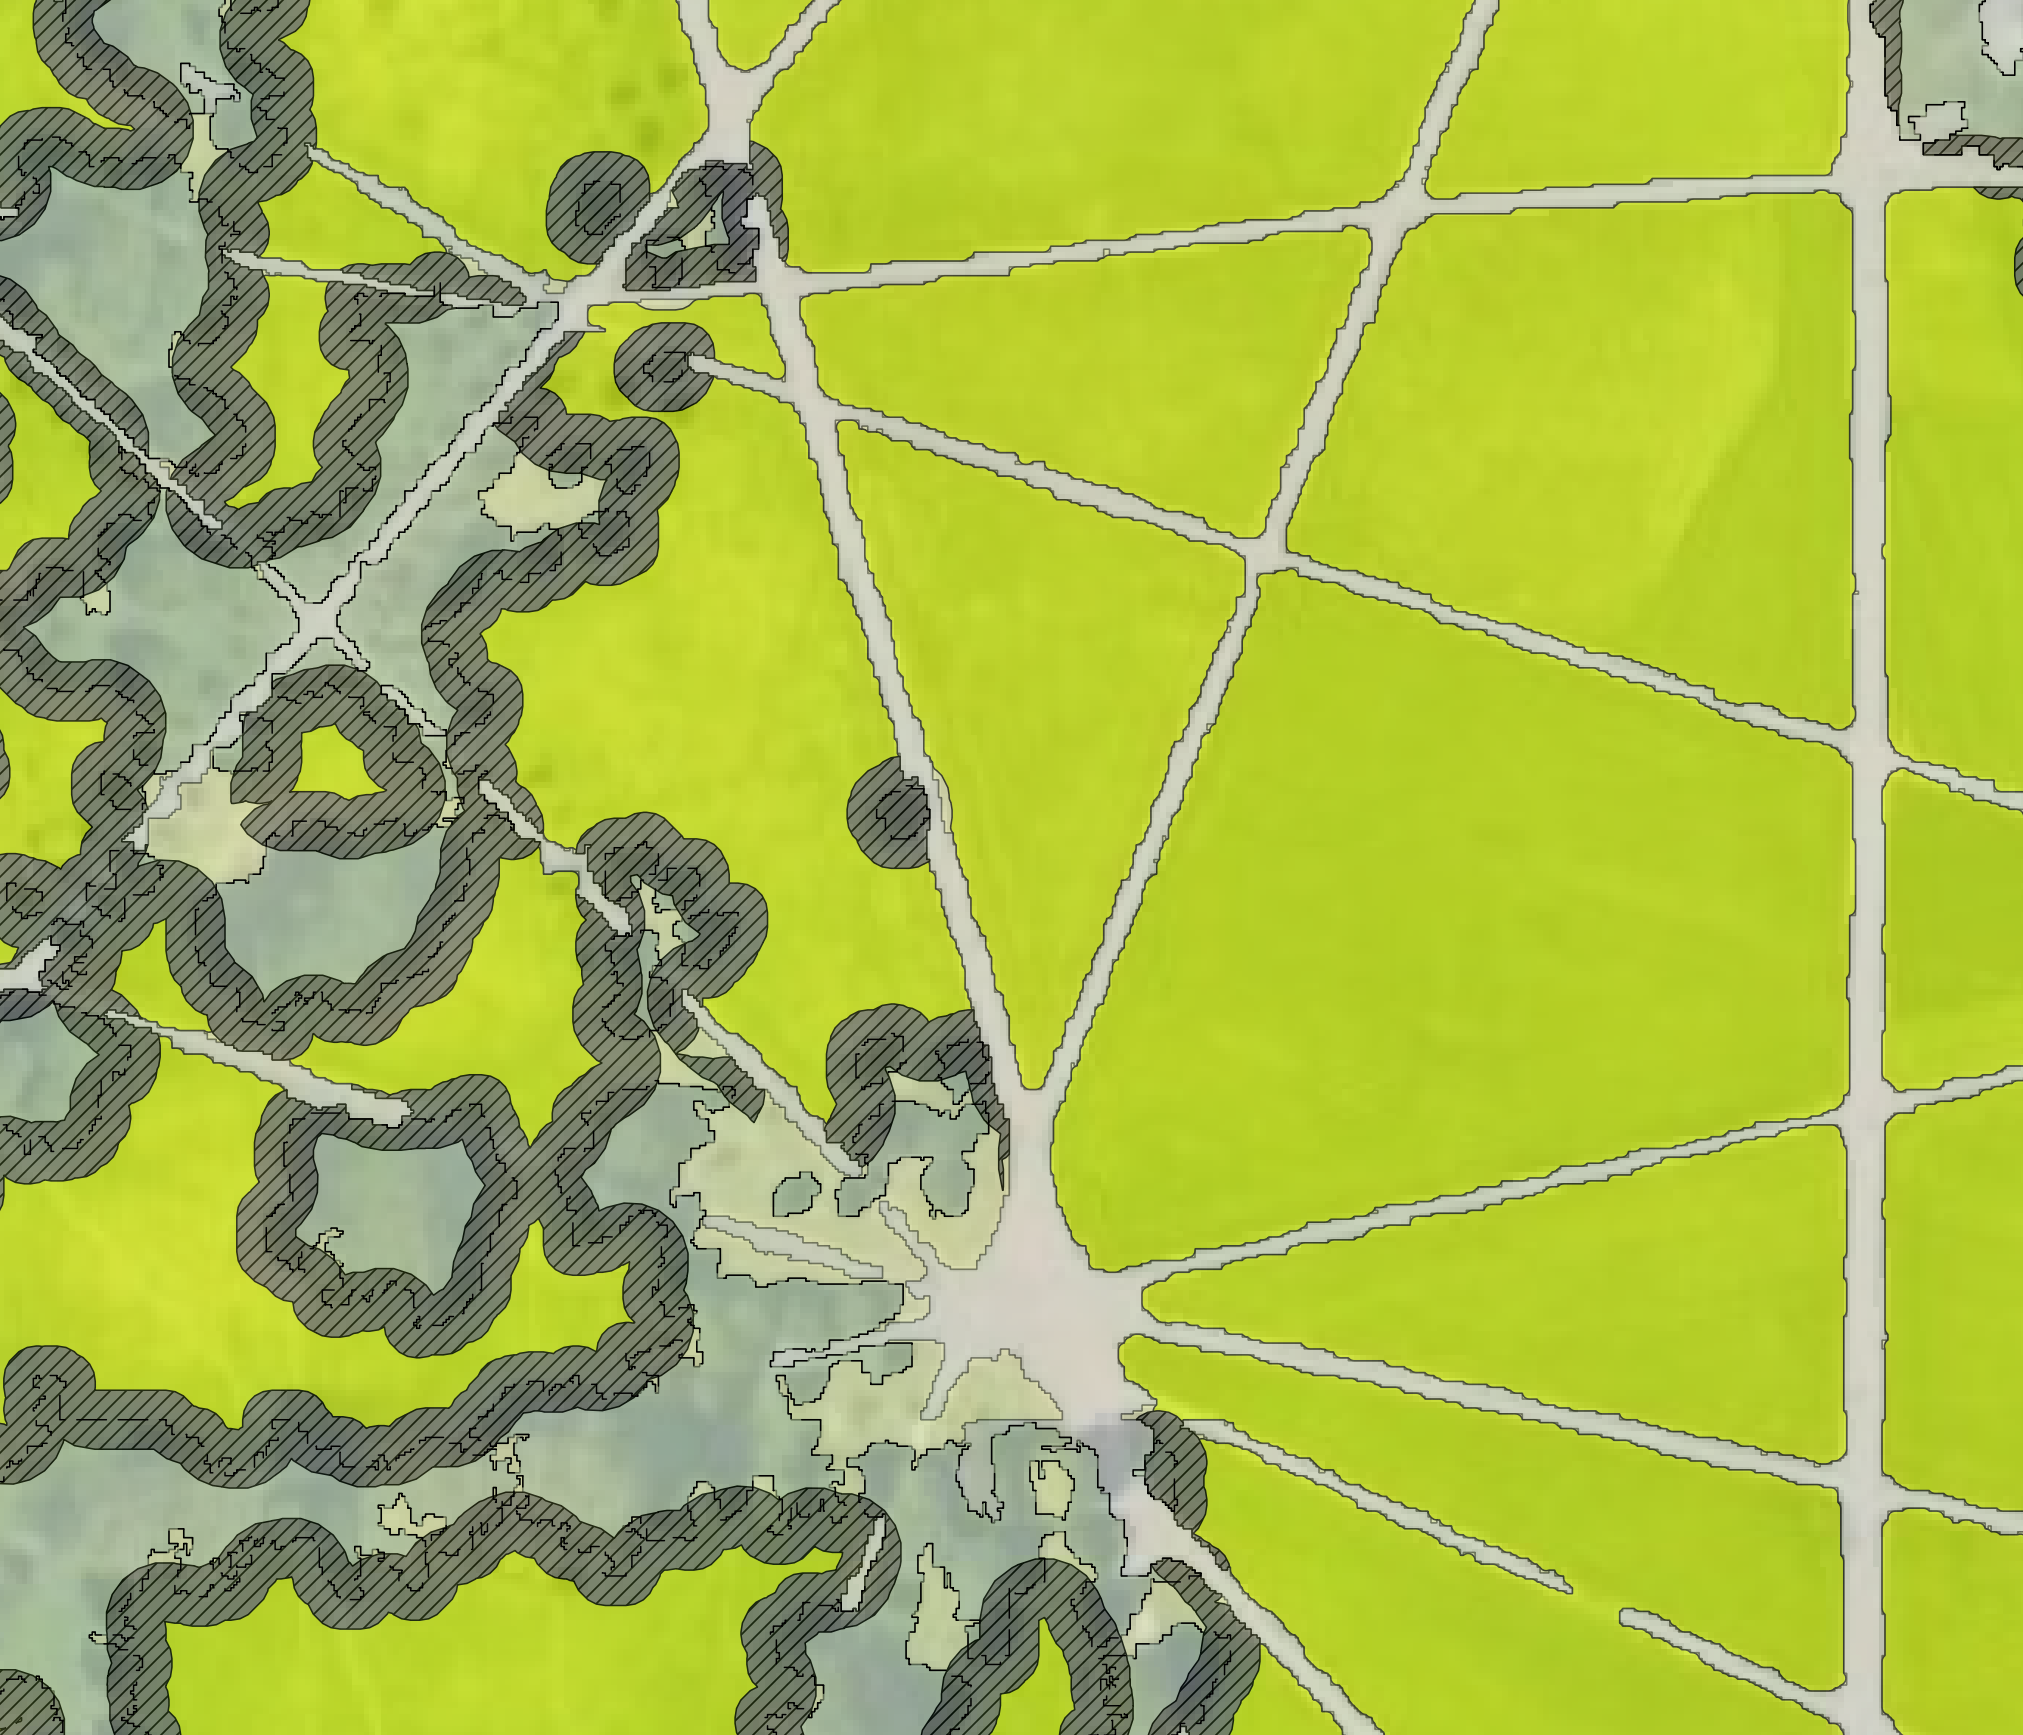
\includegraphics[width=\linewidth]{images/gatherings/hyde_locations_1000.png}\par\hspace{3pt} 
    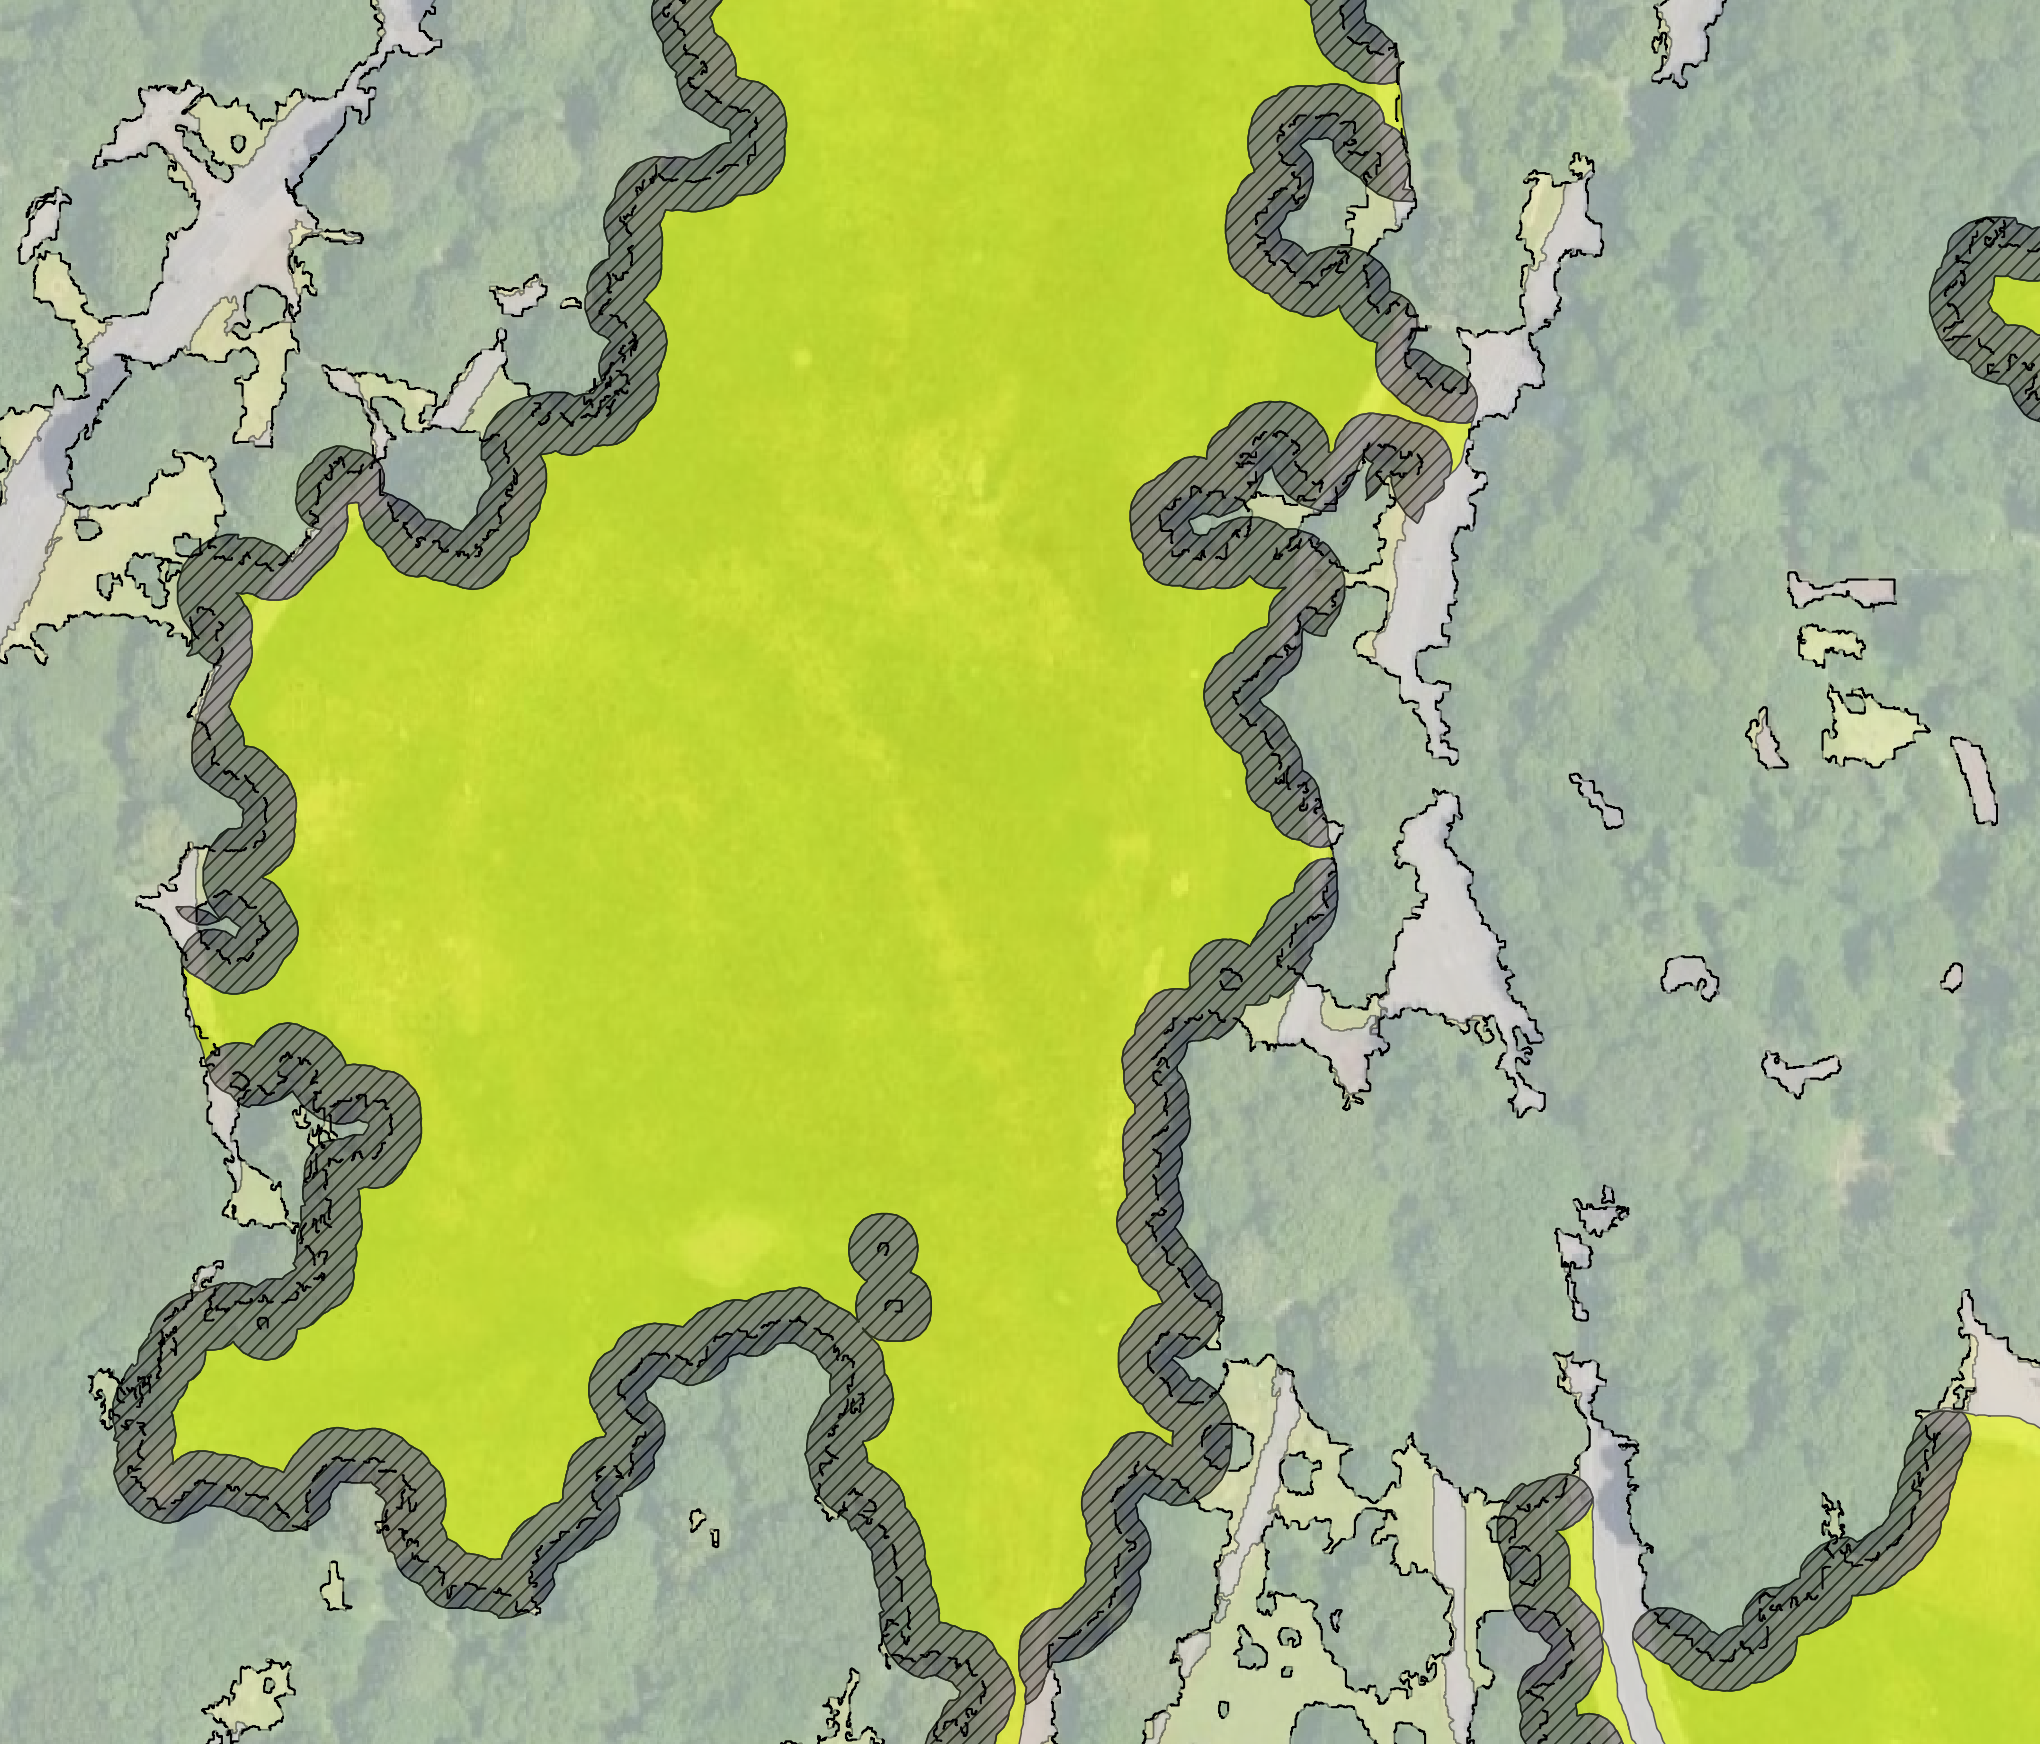
\includegraphics[width=\linewidth]{images/gatherings/prospect_locations_1000.png}\par\hspace{3pt}
    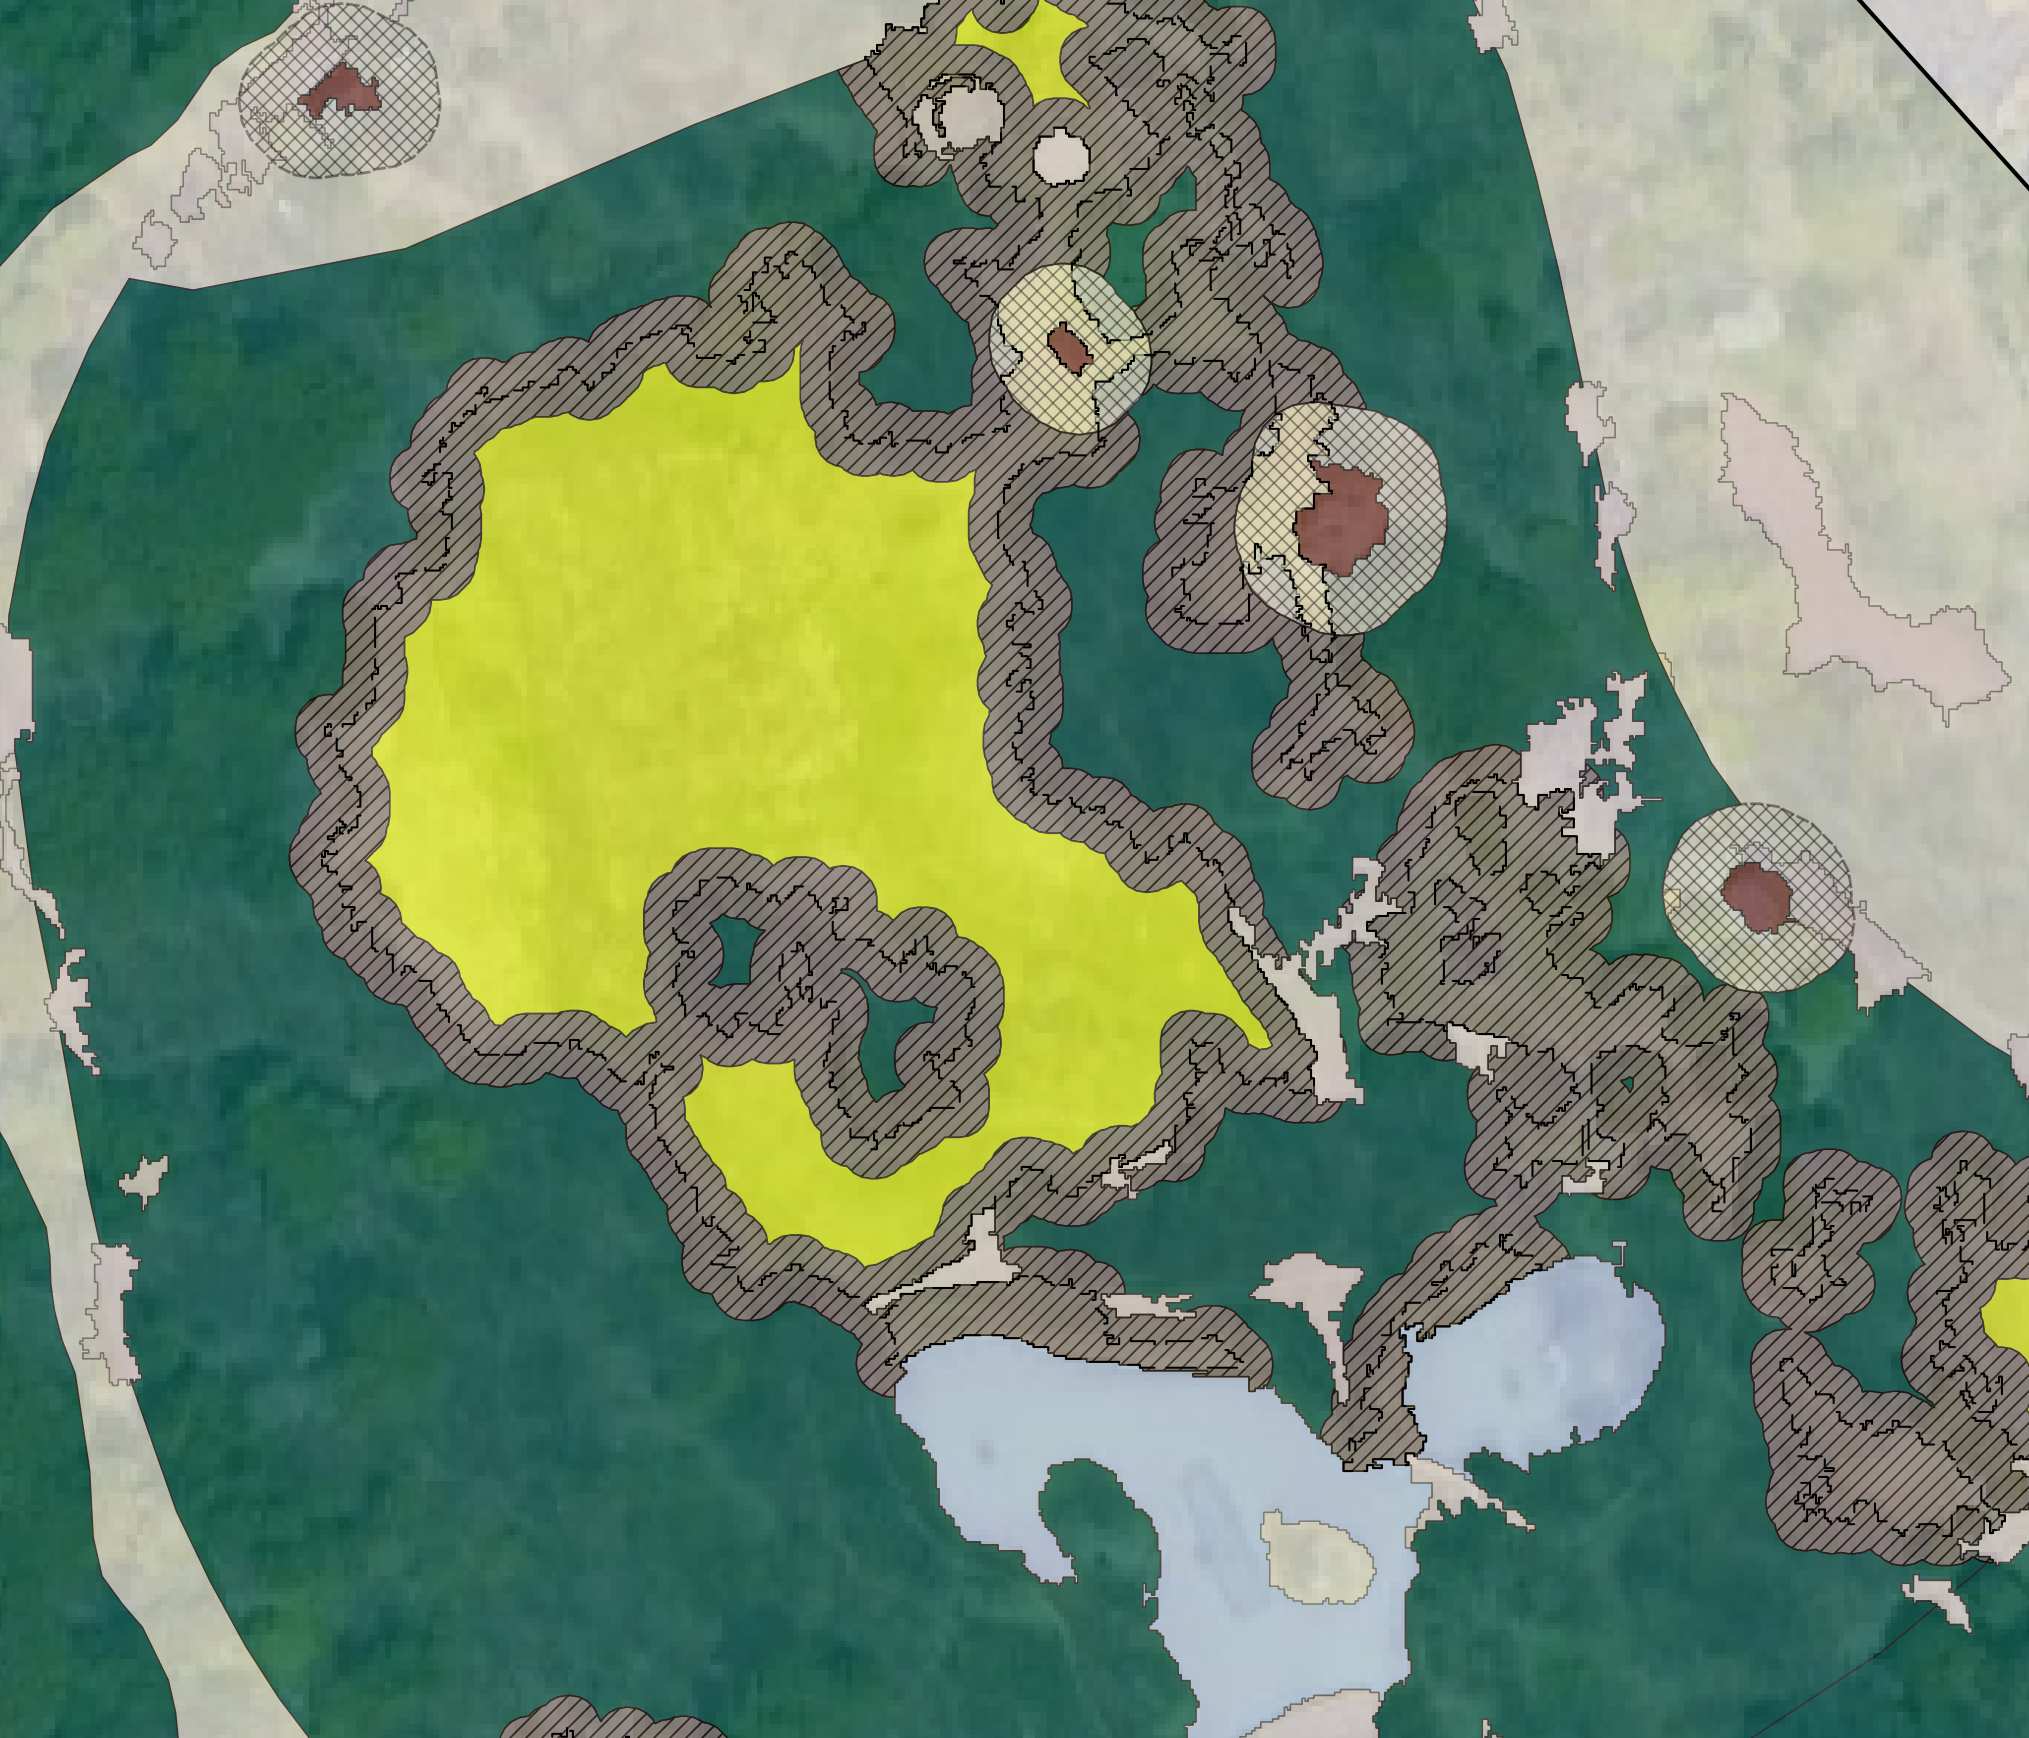
\includegraphics[width=\linewidth]{images/gatherings/yoyogi_locations_1000}\par\hspace{3pt}
    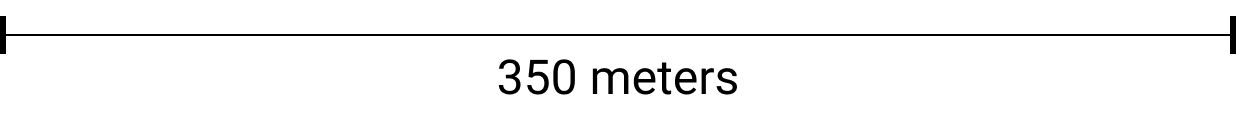
\includegraphics[width=\linewidth]{images/gatherings/scale_legend_4.png}
    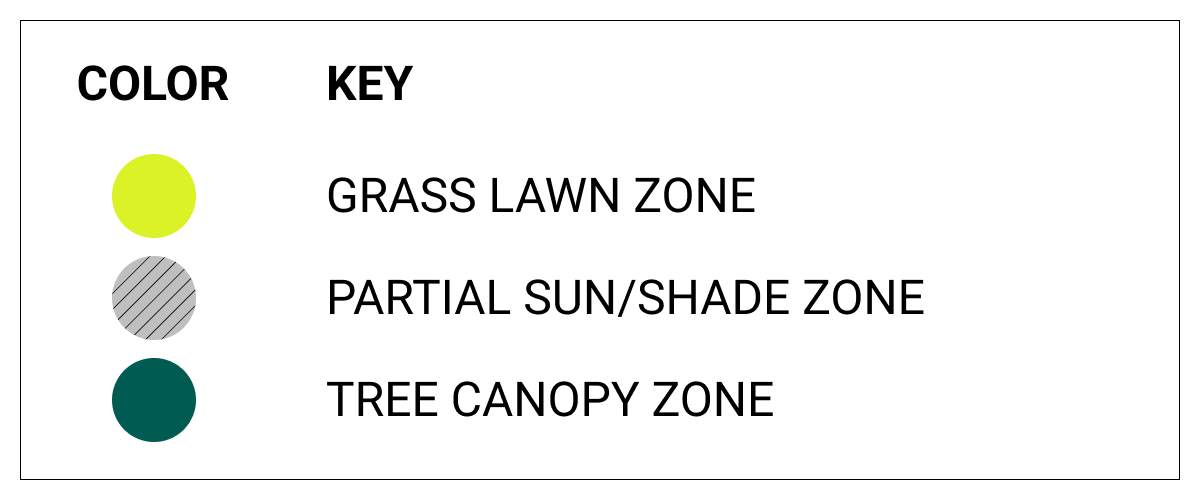
\includegraphics[width=\linewidth]{images/gatherings/gatherings_legend_2.png}
    \par\captionof{figure}[Enlarged gathering zones]{Enlarged view of gathering zones for Hyde Park (top), Prospect Park (middle) and Yoyogi Park (bottom).}
    \label{fig:locations_1000}
\end{minipage}

\begin{minipage}{0.45\textwidth}
    \centering
    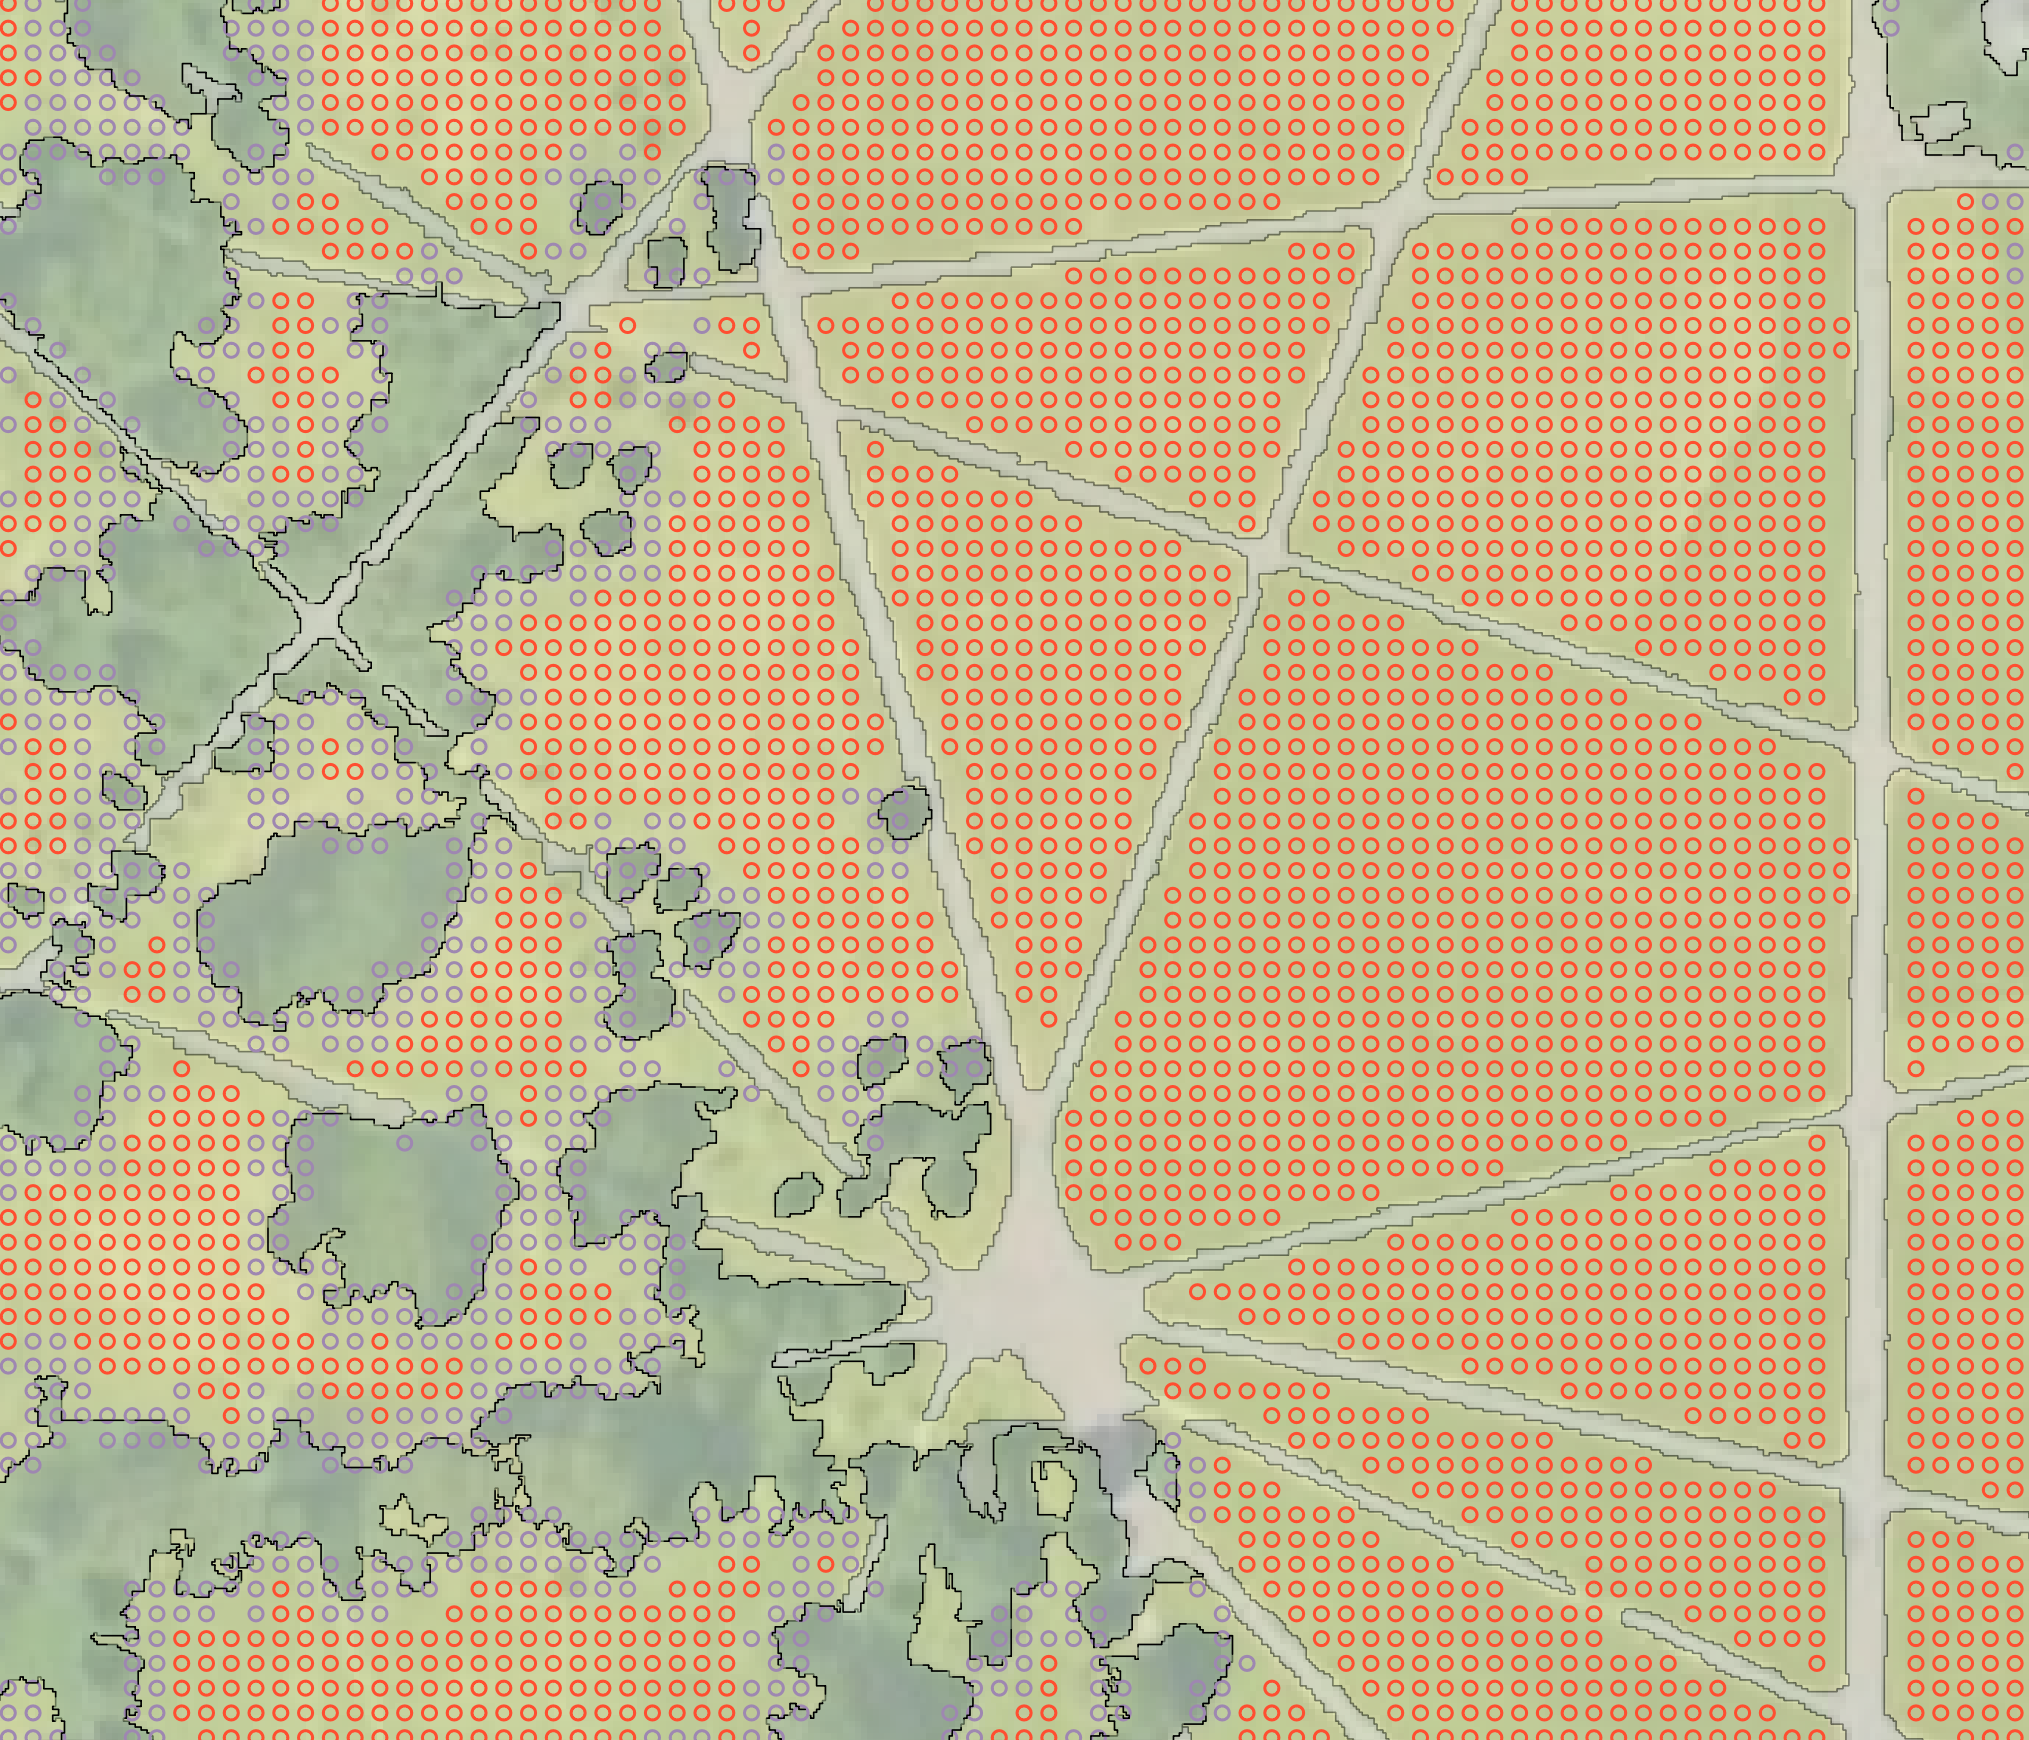
\includegraphics[width=\linewidth]{images/gatherings/hyde_circles_1000.png}\par\hspace{3pt} 
    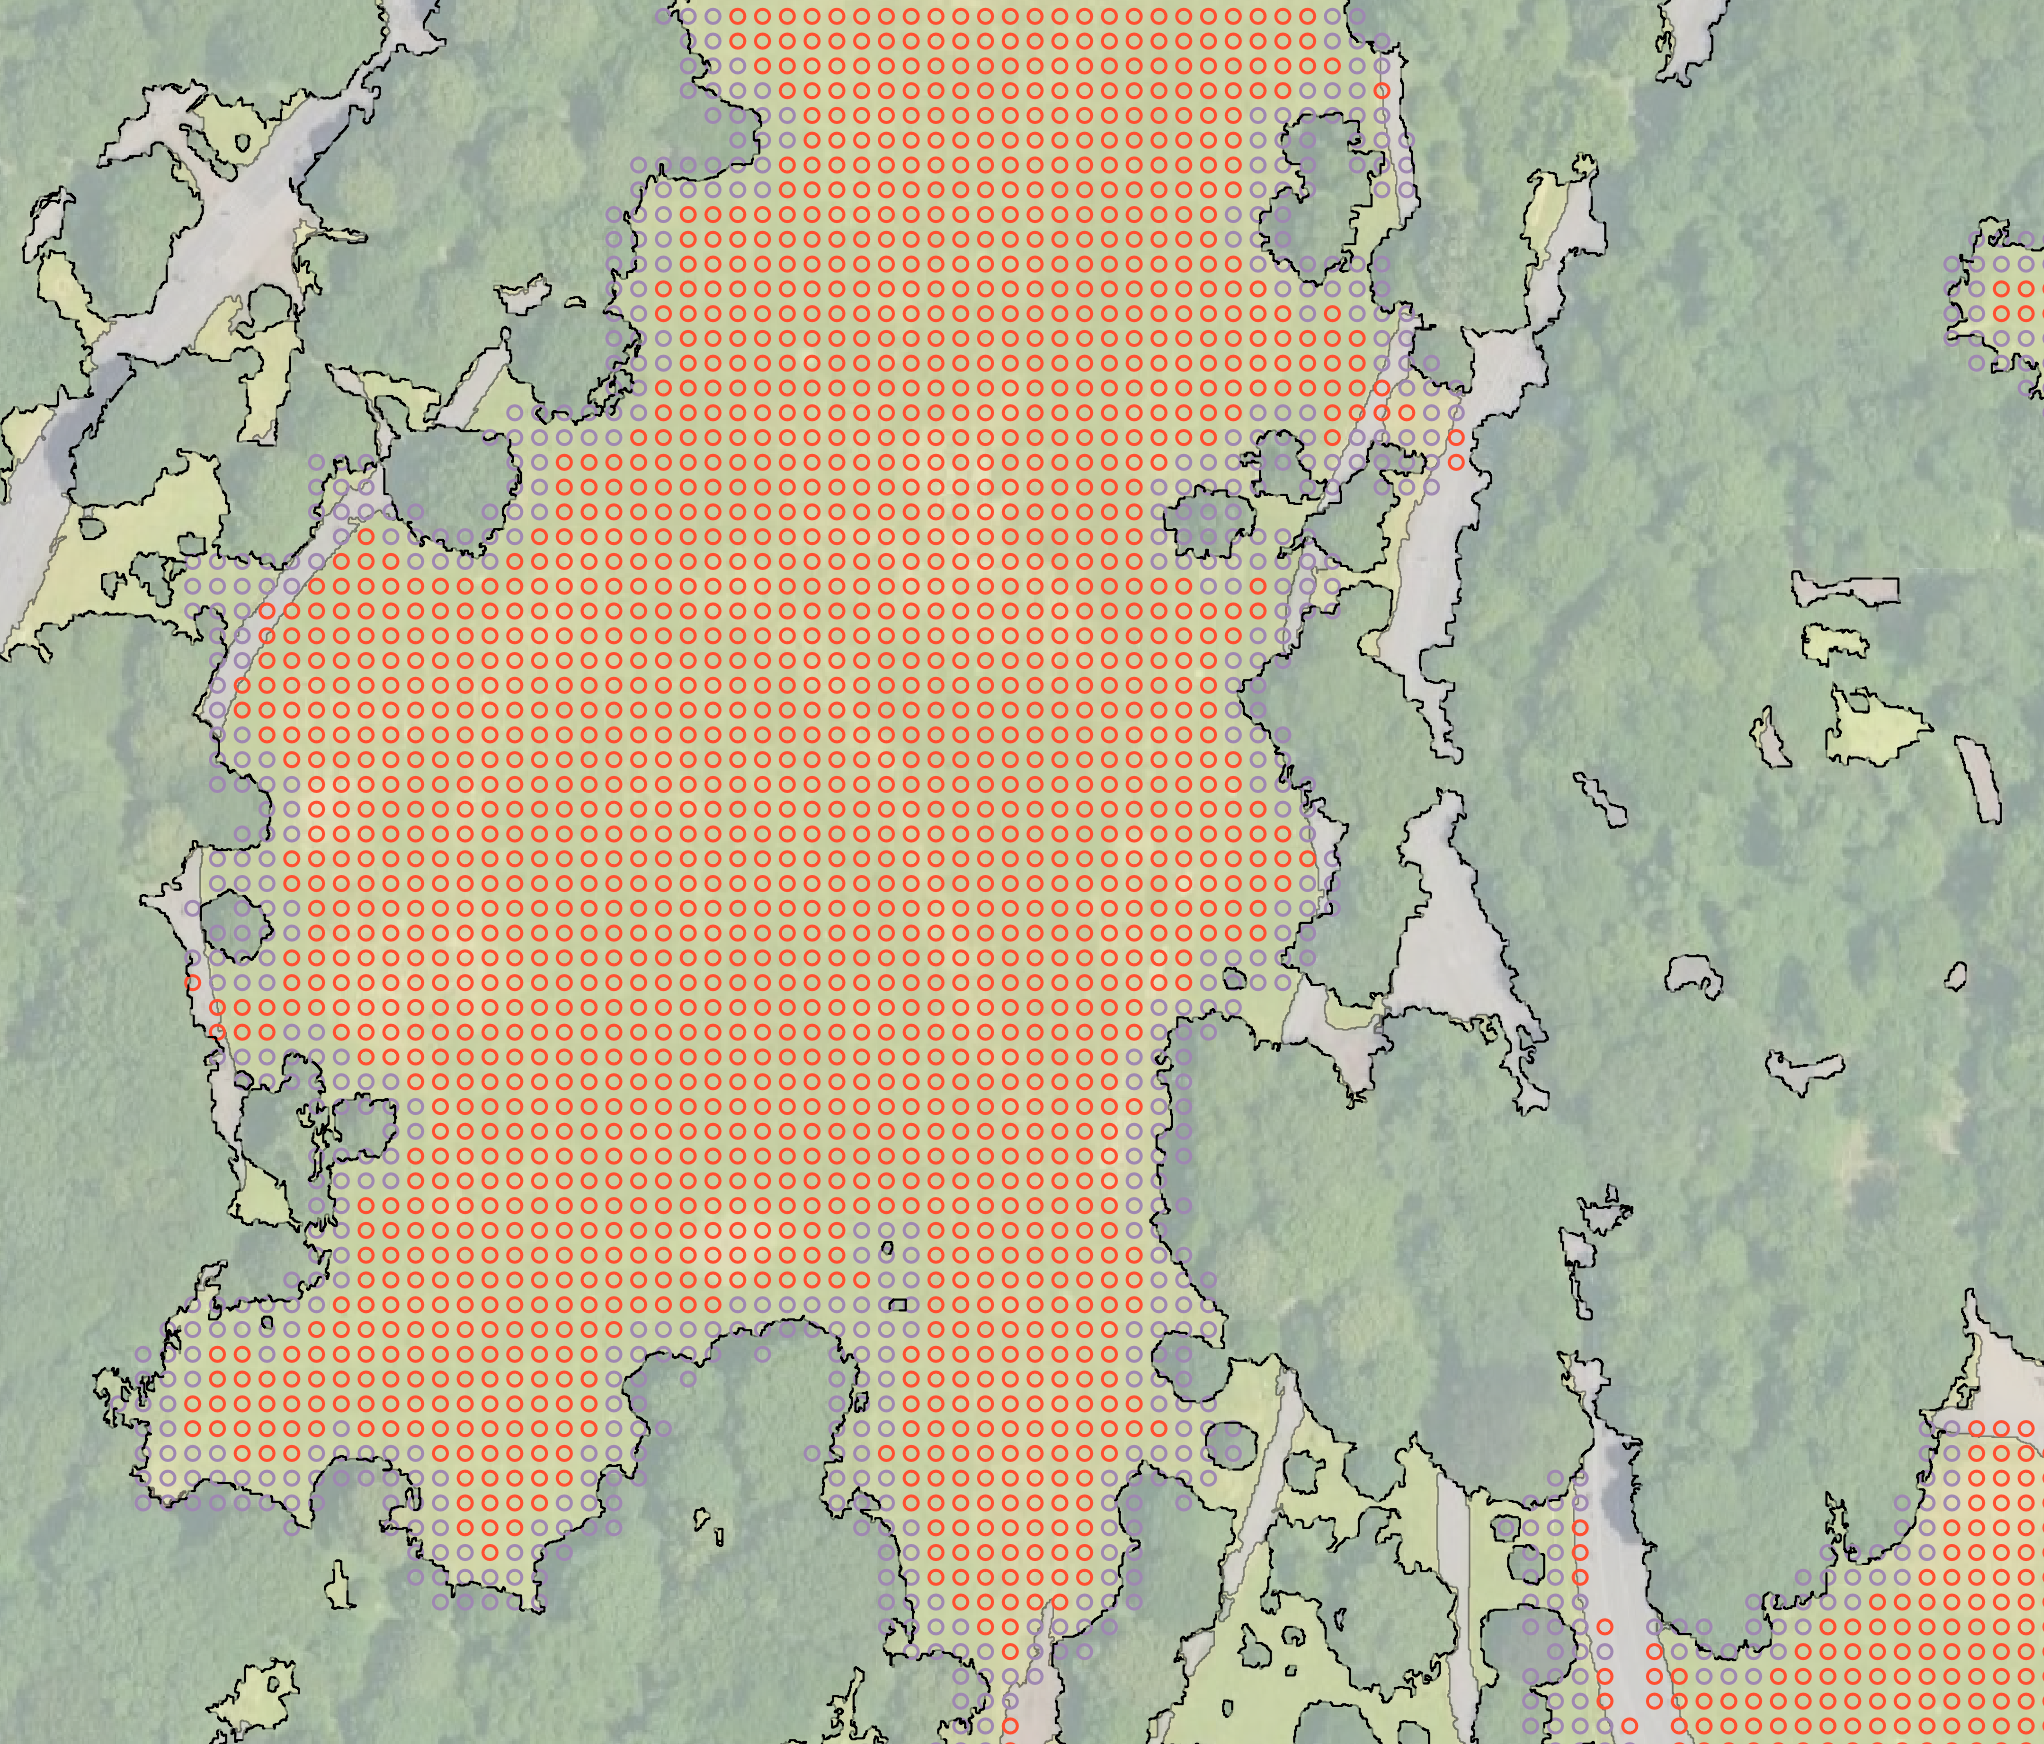
\includegraphics[width=\linewidth]{images/gatherings/prospect_circles_1000.png}\par\hspace{3pt}
    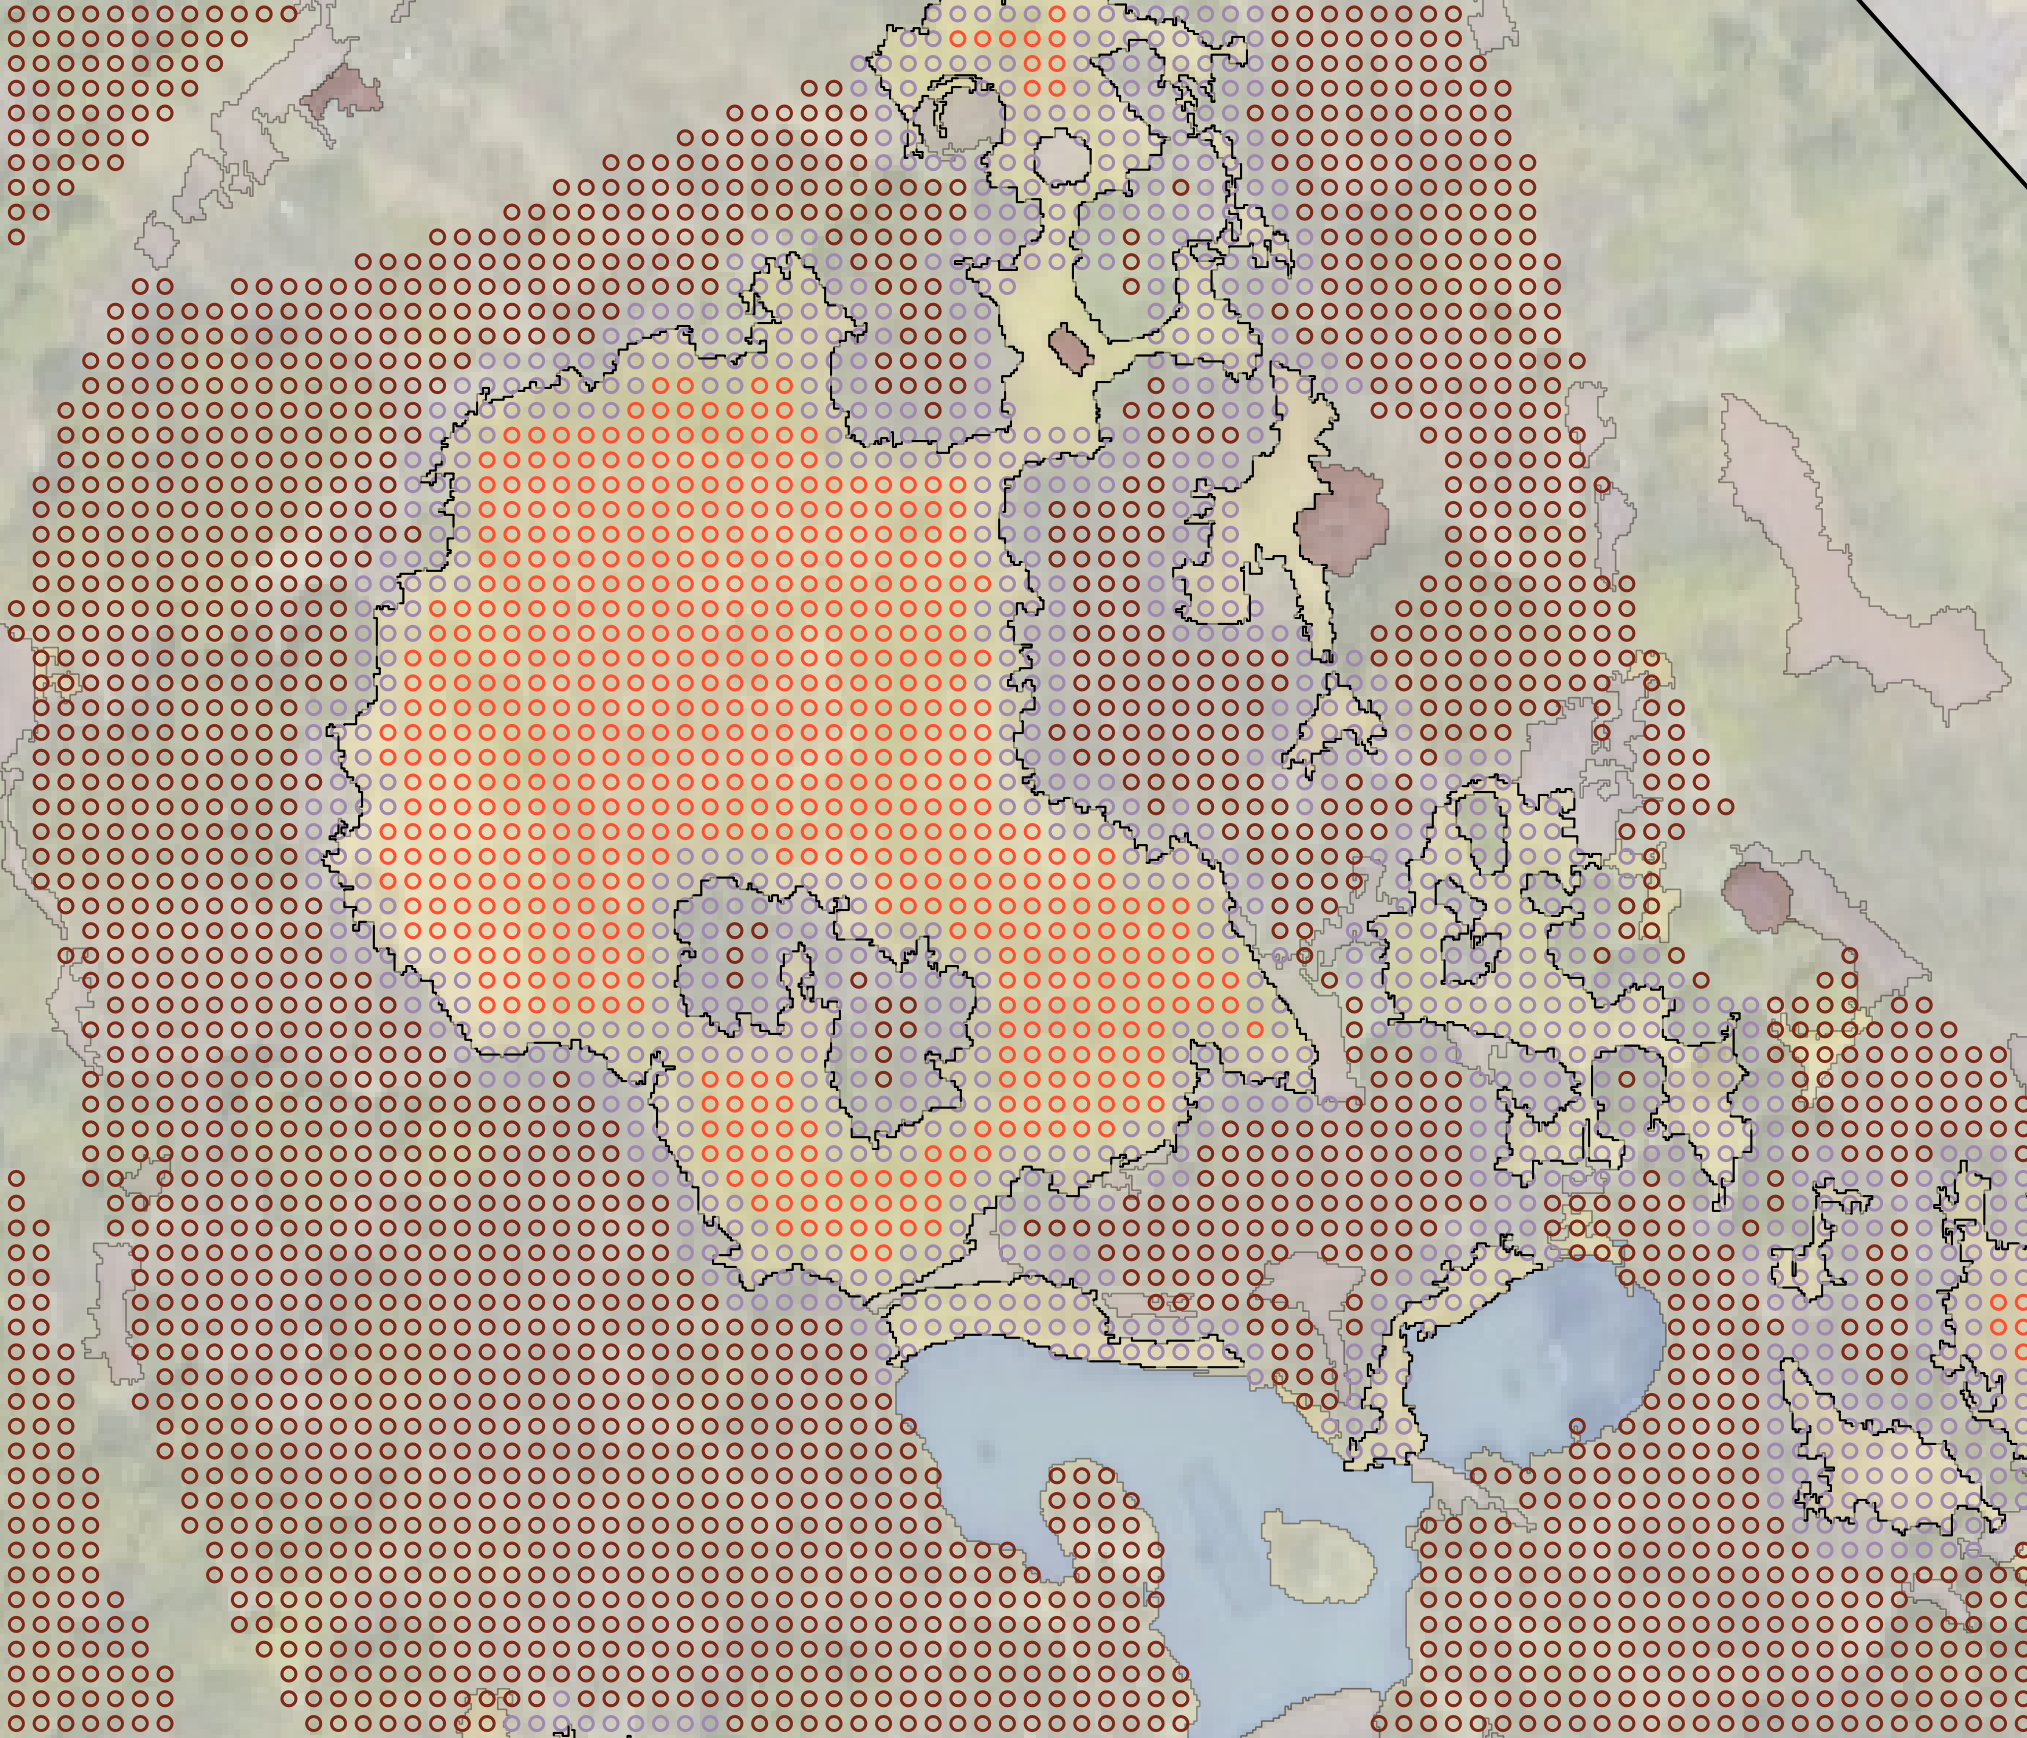
\includegraphics[width=\linewidth]{images/gatherings/yoyogi_circles_1000}\par\hspace{3pt}
    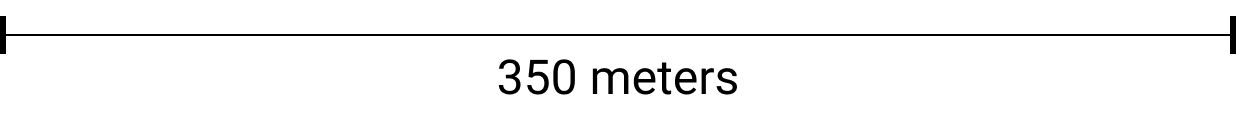
\includegraphics[width=\linewidth]{images/gatherings/scale_legend_4.png}
    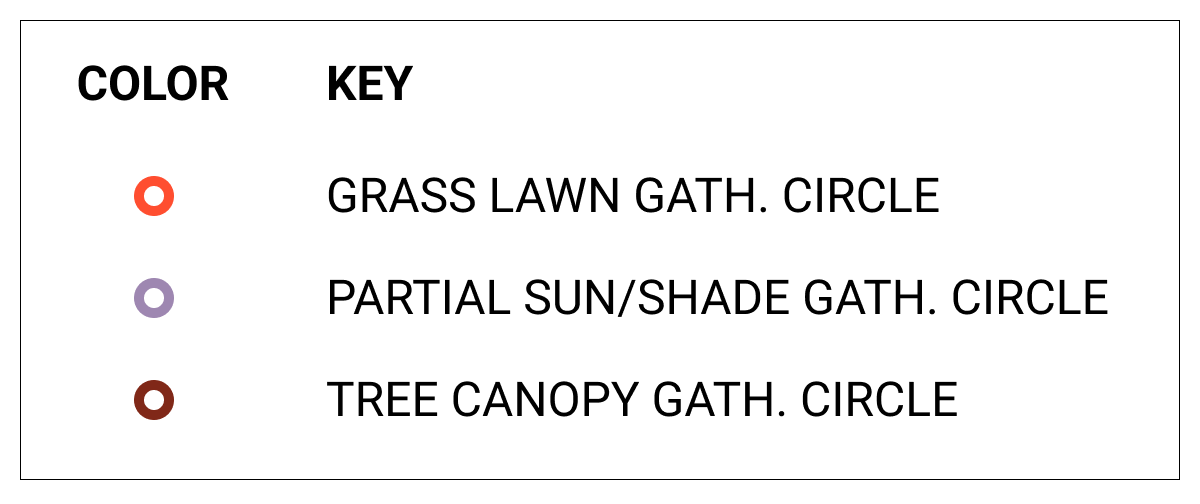
\includegraphics[width=\linewidth]{images/gatherings/gatherings_legend_3.png}
    \par\captionof{figure}[Enlarged gathering circles]{Enlarged view of gathering circles by zone for Hyde Park (top), Prospect Park (middle) and Yoyogi Park (bottom).}
    \label{fig:circles_1000}
\end{minipage}

\end{multicols}

%\begin{multicols}{2}

%\end{multicols}

 \begin{figure}[h!]
  \centering
  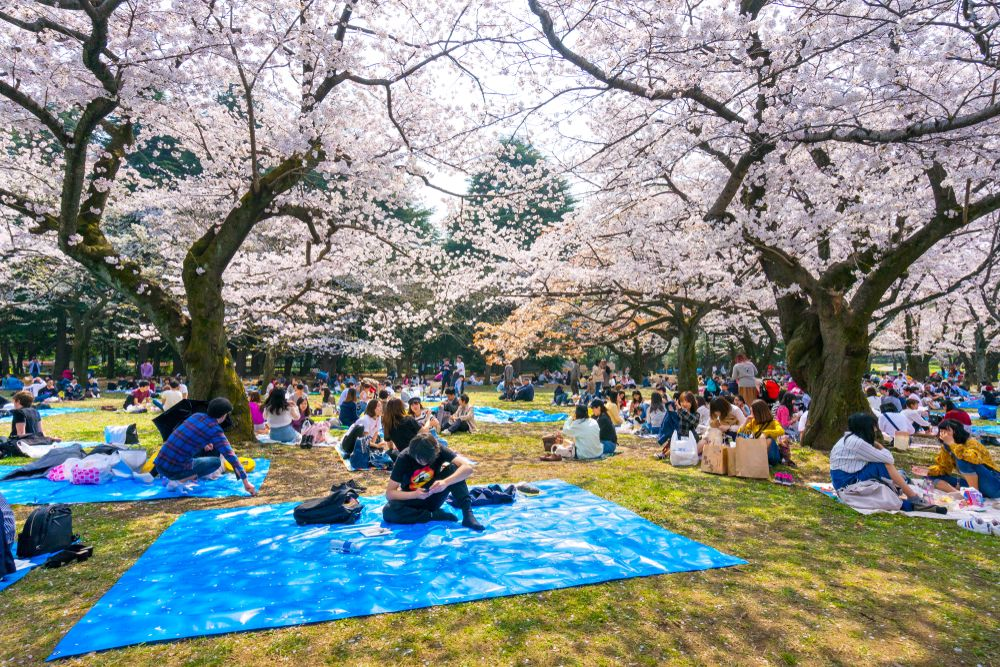
\includegraphics[width=1.0\textwidth]{images/gatherings/yoyogi3.jpeg}
  \captionsetup{width=1.0\linewidth}
  \caption[Yoyogi Park - cherry blossoms]{Image of outdoor gatherings in Yoyogi Park during cherry blossom season \cite{jrailpass_yoyogi_2019}.}
  \label{fig:yoyogi_park_cherry}
\end{figure}

\begin{multicols}{2}

\subsection{Using the results}
The three parks included in this study are both destinations for regional and international tourists as well as neighborhood parks for the people living in the surrounding areas. During a pandemic, when tourism is prohibited and even local travel is discouraged, the residents who live near these parks will be the only people able to use the public space as respite from lockdown orders. In the following chapter the number of gathering spaces calculated above will be compared against the number of people living around the parks. Additionally, access to food on the way to the park will be quantified because the ideal outdoor social gathering---most commonly referred to as the picnic---would not be complete without a meal. 

Using Domino Park as a case study, the maximum number of outdoor gatherings that can be physically drawn for park visitors during a future pandemic is quantified in this chapter (see Table \ref{gatherings_count}). By creating dedicated areas for individual use with appropriate spacing for social distancing, residents will feel safe using park space despite an ongoing public health crisis. The analysis completed here could have been accomplished in many different ways, possibly yielding different results, but the methods described above provide a starting point for future discussions about gathering spaces as a place for low-risk social interaction during a pandemic. By knowing the current social gathering capacity of existing city parks, it becomes possible to make design changes to allow for more of these spaces while possibly removing underutilized programming of city parks. 

Finally, parks are more likely to be close to capacity on days when the weather is especially nice or in the case of Tokyo, when cherry blossoms are in bloom. Even during non-pandemic times, the case can be made for knowing a park's social gathering capacity so that a park could be utilized to its full potential during the ideal day for a picnic.
\end{multicols}